%! Author = itgramic
%! Date = 11.10.23

% Preamble
%\printglossary
{
    \hypersetup{hidelinks}
    \listoffigures
}
\pagestyle{headings}
\thispagestyle{fancy}
{
    \hypersetup{hidelinks}
%\thispagestyle{fancy}
    \listoftables
    \thispagestyle{fancy}
}
{
    \hypersetup{hidelinks}
    \lstlistoflistings
    \thispagestyle{fancy}
}
\pagestyle{headings}
\thispagestyle{fancy}
%\begin{thebibliography}{XX}
%    \bibitem[XY]{XY} blah
%\clearpage
%\thispagestyle{fancy}
{
%    \renewcommand*\printbibliography{\thispagestyle{fancy}}
    \cleardoublepage
%    \pagestyle{headings}
%    \thispagestyle{fancy}
%    \renewcommand{\bibname}{\thispagestyle{fancy}}
%    \renewcommand{\biblatex}{\thispagestyle{fancy}}
%    \renewcommand{\bibpreamble}{\thispagestyle{fancy}}
    \renewcommand{\bibsetup}{\thispagestyle{fancy}}
%    \bibliographystyle{ieeetr}
    \printbibliography
%    \pagestyle{headings}
%    \thispagestyle{fancy}
}
\begin{flushleft}
    \cleardoublepage
    \renewcommand{\bibsetup}{\thispagestyle{fancy}}
    %! Author = itgramic
%! Date = 03.10.23

% Preamble
\begin{abkuerzungen}[MUSTER] % Das Muster dient zur Bestimmung der Einrueckungstiefe
    \item[ICT] information and communications technology
    \item[ibW] ibW Höhere Fachschule Südostschweiz
    \item[KSGR] Kantonsspital Graubünden
    \item[KPS] KSGR Provisioning System
    \item[\Gls{RDBMS}] Relational Database Management System
    \item[\Gls{DBMS}] Database Mananagement System
    \item[k8s] \Gls{Kubernetes}
    \item[HPE] Hewlett Packard Enterprise
    \item[\Gls{HP-UX}] Hewlett Packard \Gls{UNIX}
    \item[SAP] Systemanalyse Programmentwicklung
    \item[SQL] Structured Query Language
    \item[DBA] Database Administrator / Datenbankadministrator
    \item[HA] High Availability
    \item[\Gls{PRTG}] Paessler Router Traffic Grapher
    \item[\Gls{SAN}] Storage Area Network
    \item[\Gls{SIEM}] Security Information and Event Management
    \item[\Gls{CI/CD}] Continuous Integration/Continuous Delivery
    \item[\Gls{SWOT}] Strengths, Weaknesses, Opportunities, Threats
    \item[\Gls{OLAP}] Online Analytical Processing
    \item[IaC] Infrastructure as Code
    \item[IPERKA] Informieren, Planen, Entscheiden, Realisieren, Kontrollieren, Auswerten
    \item[BSI] Bundesamt für Sicherheit in der Informationstechnik
    \item[\Gls{VRRP}] Virtual Router Redundancy Protocol
    \item[\Gls{PKI}] Private Key Infrastructure
    \item[\Gls{DCS}] Distributed Configuration Store
    \item[DQL] Data Query Language
    \item[DML] Data Manipulation Language
    \item[ACID] Atomicity, Consistency, Isolation und Durability
    \item[EDB] EnterpriseDB
    item[CRD] Custom Resource Definition
\end{abkuerzungen}
\end{flushleft}
{
%    \renewcommand{\glossarymark}[1]{}
%    \cleardoublepage
%    \thispagestyle{fancy}
    \renewcommand*\glossarypreamble{\thispagestyle{fancy}}
    \printnoidxglossaries
}
{
    %\printindex
}


%\makeindex
%\printglossary[type=\acronymtype]
\begin{appendix}
%   \printglossary


        \begin{flushleft}
        \chapter*{Selbstständigkeitserklärung}
        Ich versichere, dass die vorliegende Arbeit von den Autoren selbständig und ohne Benutzung anderer als der angegebenen Hilfsmittel angefertigt wurde.
        Alle Inhalte dieser Arbeit, dazu gehören neben Texten auch Grafiken, Programmcode, etc.,
        die wörtlich oder sinngemäss aus anderen Quellen stammen, sind als solche eindeutig kenntlich gemacht und korrekt im Quellenverzeichnis gelistet.
        Dies gilt auch für einzelne Auszüge aus fremden Quellen.
        \end{flushleft}
        \begin{flushleft}
        Die Arbeit ist in gleicher oder ähnlicher Form noch nicht veröffentlicht und noch keiner Prüfungsbehörde vorgelegt worden.

        \vspace{4cm}
        \noindent
        \hrule \ \\[-0.5ex]
        Ort, Datum, Unterschrift
        \end{flushleft}
        \begin{flushleft}
        \chapter*{Haftungsausschluss}
        Der vorliegende Bericht wurde von Studierenden im Rahmen einer Diplomarbeit erarbeitet.
        Es muss an dieser Stelle darauf hingewiesen werden, dass die Arbeit nicht im Rahmen eines Auftragsverhältnisses erstellt wurde.
        Weder der Ersteller noch die ibW Höhere Fachhochschule Südostschweiz können deshalb für Aktivitäten auf der Basis dieser Diplomarbeit eine Haftung übernehmen.
        \end{flushleft}

    \renewcommand{\thesection}{\Roman{section}}
    \renewcommand{\thesubsection}{\thesection.\Roman{subsection}}
    \renewcommand{\thesubsubsection}{\thesubsection.\Roman{subsubsection}}
    \renewcommand{\theparagraph}{\thesubsubsection.\Roman{paragraph}}
    \renewcommand{\thesubparagraph}{\theparagraph.\Roman{subparagraph}}

    \titleformat{\section}[block]{\filright\normalfont\normalsize\normalcolor\fontsize{11.5pt}{13.8pt}\selectfont\sffamily\bfseries\color[HTML]{000000}}{{\fontsize{11pt}{14.400001pt}\selectfont \makebox[2.5cm][l]{\thesection}}}{0pt}{#1}[]
    \titlespacing*{\section}{0pt}{0.847cm plus 0.1694cm minus 0.0847cm}{0.212cm plus 0.0424cm minus 0.0212cm}
    \titleformat{\subsection}[block]{\filright\normalfont\normalsize\normalcolor\fontsize{10pt}{13.8pt}\selectfont\sffamily\bfseries\color[HTML]{000000}}{{\fontsize{11pt}{14.400001pt}\selectfont \makebox[2.5cm][l]{\thesubsection}}}{0pt}{#1}[]
    \titlespacing*{\subsection}{0pt}{0.847cm plus 0.1694cm minus 0.0847cm}{0.212cm plus 0.0424cm minus 0.0212cm}
    \titleformat{\subsubsection}[block]{\filright\normalfont\normalsize\normalcolor\fontsize{10pt}{13.8pt}\selectfont\sffamily\bfseries\color[HTML]{000000}}{{\fontsize{11pt}{14.400001pt}\selectfont \makebox[2.5cm][l]{\thesubsubsection}}}{0pt}{#1}[]
    \titlespacing*{\subsubsection}{0pt}{0.847cm plus 0.1694cm minus 0.0847cm}{0.212cm plus 0.0424cm minus 0.0212cm}
%    \titleformat{\subsubsection}[block]{\filright\normalfont\normalsize\normalcolor\fontsize{10pt}{13.8pt}\selectfont\sffamily\bfseries\color[HTML]{000000}}{{\fontsize{11pt}{14.400001pt}\selectfont \makebox[2.5cm][l]{\thesubsubsection}}}{0pt}{#1}[]
%    \titlespacing*{\subsubsection}{0pt}{0.847cm plus 0.1694cm minus 0.0847cm}{0.212cm plus 0.0424cm minus 0.0212cm}
    \titleformat{\paragraph}[block]{\filright\normalfont\normalsize\normalcolor\fontsize{10pt}{13.8pt}\selectfont\sffamily\bfseries\color[HTML]{000000}}{{\fontsize{11pt}{14.400001pt}\selectfont \makebox[2.5cm][l]{\theparagraph}}}{0pt}{#1}[]
    \titlespacing*{\paragraph}{0pt}{0.847cm plus 0.1694cm minus 0.0847cm}{0.212cm plus 0.0424cm minus 0.0212cm}
    \titleformat{\subparagraph}[block]{\filright\normalfont\normalsize\normalcolor\fontsize{10pt}{13.8pt}\selectfont\sffamily\bfseries\color[HTML]{000000}}{{\fontsize{11pt}{14.400001pt}\selectfont \makebox[2.5cm][l]{\thesubparagraph}}}{0pt}{#1}[]
    \titlespacing*{\subparagraph}{0pt}{0.847cm plus 0.1694cm minus 0.0847cm}{0.212cm plus 0.0424cm minus 0.0212cm}

    \captionsetup[table]{name=Tabelle}
    \renewcommand{\thetable}{\Roman{table}}
    \captionsetup[figure]{name=Abbildung}
    \renewcommand{\thefigure}{\Roman{figure}}

    \clearpage
    \addcontentsline{toc}{chapter}{Anhang}
    \addtocontents{toc}{%
    \protect\addtokomafont{chapterentry}{Anhang\ }
%    \pagenumbering{roman}
%    \setcounter{page}{1}
    }
    \pagenumbering{roman}
    \setcounter{page}{1}
%\listofatoc
%\tableofcontents
%    %! Author = itgramic
%! Date = 12.01.24

% Preamble
\section{Statusbericht}
\subsection{}
    %! Author = itgramic
%! Date = 05.01.24

% Preamble
\newpage
\section{Disposition}
\label{chap:disposition}
%\begin{flushleft}
%    \begin{figure}[H]
%        \centering
%%        
\includegraphics[width=1\linewidth]{source/appendix/Michael_Graber_Disposition_Diplomarbeit_2023_2024}
%        
\includepdf[pages={1-},scale=0.75]{source/appendix/Michael_Graber_Disposition_Diplomarbeit_2023_2024}
%        \caption{Disposition}
%        \label{fig:disposition}
%    \end{figure}

\includepdf[pages={1-},scale=0.75]{source/appendix/Michael_Graber_Disposition_Diplomarbeit_2023_2024}
%\caption{Disposition}
%\label{fig:disposition}
\captionof{figure}{Disposition}
%\end{flushleft}
    %! Author = ibw
%! Date = 10.11.23

% Preamble
\subsection{Rapport}
    %! Author = gramic
%! Date = 17.03.24
% Preamble
%\begin{landscape}
%    \begin{flushleft}
%        \section{Protokoll - Fachgespräche}
%        \begin{table}[H]

\resizebox{\columnwidth}{!}{%

\begin{tabular}{rllllllll}
\toprule
Fachgespräch & Datum & Fachexperte & Nebenexperte & Studenten & Fragen & Antworten & Sonstige Themen & Bemerkungen \\
\midrule
1 & 14.02.2024 & Norman Süsstrunk & - & \begin{tabular}[c]{@{}l@{}}Michael Graber\\Curdin Roffler\end{tabular} & \begin{tabular}[c]{@{}l@{}}- Darf eine Vorauswahl stattfinden, um den Aufwand zur reduzieren?\end{tabular} & \begin{tabular}[c]{@{}l@{}}- Eine Vorauswahl ist Sinnvoll und in diesem Rahmen fast zwingend Notwendig,\\  da sonst viel zuviel Zeit investiert werden müsste\end{tabular} & \begin{tabular}[c]{@{}l@{}}- Vorstellung Norman Süsstrunk, Curdin Roffler und Michael Graber\\- Kontaktdaten shared\\- Bei Fragen jederzeit an Norman wenden\\- Norman braucht aber mindestens 1. Woche vorlaufzeit\\- Norman wird sich spätestens zur Halbzeit melden.\\- Norman wird sic\end{tabular} & \begin{tabular}[c]{@{}l@{}}- Es wurden zwar für alle Studenten von Norman Süsstrunk Zoom-Räume bereitgestellt,\\  aus effizienzgründen nahmen Curdin Roffler und ich beide am selben Meeting teil\end{tabular} \\
2 &  & Norman Süsstrunk & - & \begin{tabular}[c]{@{}l@{}}Michael Graber\end{tabular} & \begin{tabular}[c]{@{}l@{}}- Hat Norman ggf. noch vorschläge zu PostgreSQL Clustern gefunden?\\- Soll ich die Gewichtung mit 100 Punkten machen oder 1000?\\I  m Moment haben diverse Punkte eine sehr kleine Punktzahl\\- Soll die Disposition in den Anhang?\\  Diese ist 50 Seiten lang und\end{tabular} & \begin{tabular}[c]{@{}l@{}}\end{tabular} & \begin{tabular}[c]{@{}l@{}}- Freigabe des Protokolls\end{tabular} & \begin{tabular}[c]{@{}l@{}}\end{tabular} \\
\bottomrule
\end{tabular}
}
\caption{Fachgespräche - Protokoll} \label{expert_discussions_full_list}
\end{table}

%    \end{flushleft}
%\end{landscape}
\begin{flushleft}
    \section{Protokoll - Fachgespräche}
%    \begin{table}[H]

\resizebox{\columnwidth}{!}{%

\begin{tabular}{rllllllll}
\toprule
Fachgespräch & Datum & Fachexperte & Nebenexperte & Studenten & Fragen & Antworten & Sonstige Themen & Bemerkungen \\
\midrule
1 & 14.02.2024 & Norman Süsstrunk & - & \begin{tabular}[c]{@{}l@{}}Michael Graber\\Curdin Roffler\end{tabular} & \begin{tabular}[c]{@{}l@{}}- Darf eine Vorauswahl stattfinden, um den Aufwand zur reduzieren?\end{tabular} & \begin{tabular}[c]{@{}l@{}}- Eine Vorauswahl ist Sinnvoll und in diesem Rahmen fast zwingend Notwendig,\\  da sonst viel zuviel Zeit investiert werden müsste\end{tabular} & \begin{tabular}[c]{@{}l@{}}- Vorstellung Norman Süsstrunk, Curdin Roffler und Michael Graber\\- Kontaktdaten shared\\- Bei Fragen jederzeit an Norman wenden\\- Norman braucht aber mindestens 1. Woche vorlaufzeit\\- Norman wird sich spätestens zur Halbzeit melden.\\- Norman wird sic\end{tabular} & \begin{tabular}[c]{@{}l@{}}- Es wurden zwar für alle Studenten von Norman Süsstrunk Zoom-Räume bereitgestellt,\\  aus effizienzgründen nahmen Curdin Roffler und ich beide am selben Meeting teil\end{tabular} \\
2 &  & Norman Süsstrunk & - & \begin{tabular}[c]{@{}l@{}}Michael Graber\end{tabular} & \begin{tabular}[c]{@{}l@{}}- Hat Norman ggf. noch vorschläge zu PostgreSQL Clustern gefunden?\\- Soll ich die Gewichtung mit 100 Punkten machen oder 1000?\\I  m Moment haben diverse Punkte eine sehr kleine Punktzahl\\- Soll die Disposition in den Anhang?\\  Diese ist 50 Seiten lang und\end{tabular} & \begin{tabular}[c]{@{}l@{}}\end{tabular} & \begin{tabular}[c]{@{}l@{}}- Freigabe des Protokolls\end{tabular} & \begin{tabular}[c]{@{}l@{}}\end{tabular} \\
\bottomrule
\end{tabular}
}
\caption{Fachgespräche - Protokoll} \label{expert_discussions_full_list}
\end{table}

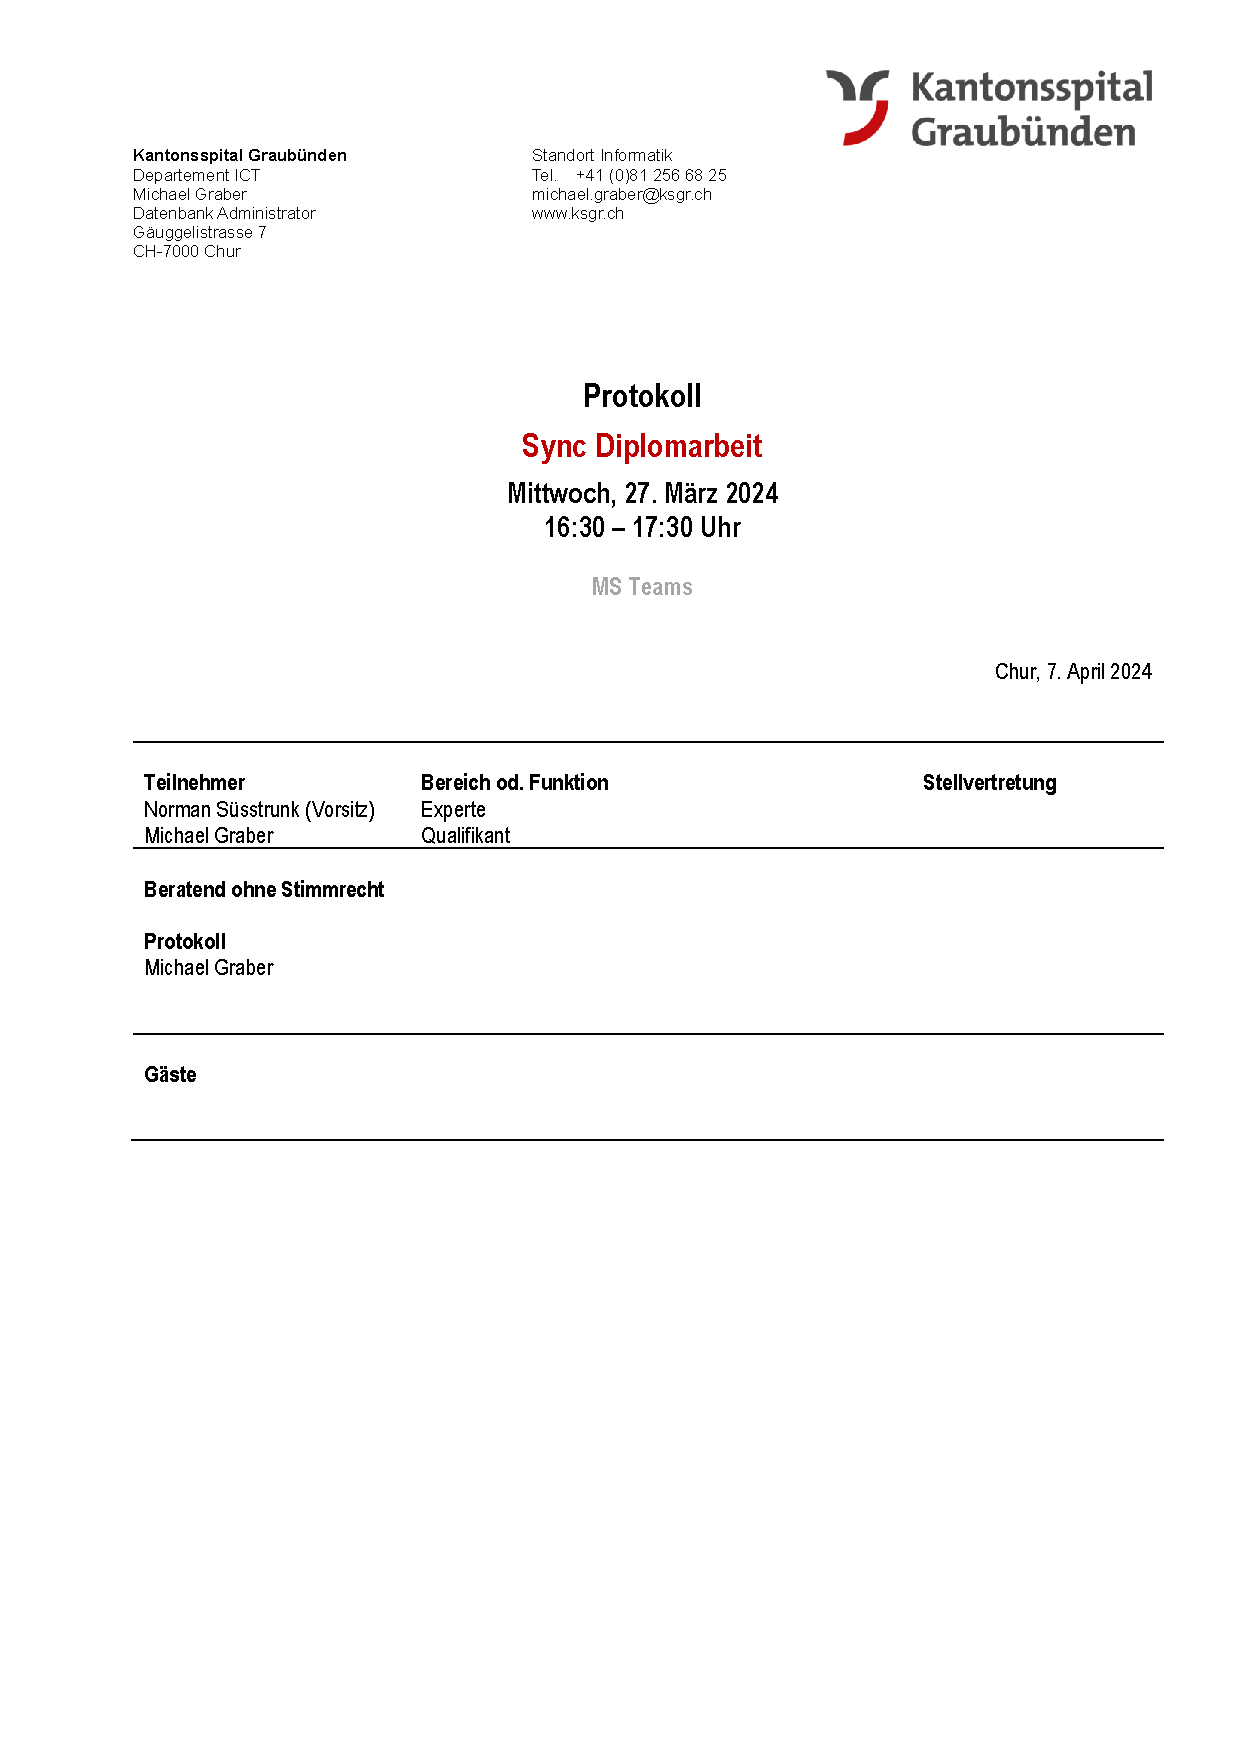
\includepdf[pages=1-,pagecommand={\subsection{Fachgespräch 27.03.2024}}, fitpaper=true,scale=0.9]{source/projectmanagement_overhead/projectmanagement/expert_discussions/protokoll_expertengespraech_27.03.2024.pdf}
\end{flushleft}
    %! Author = itgramic
%! Date = 12.01.24

% Preamble
\section{Statusbericht}
\subsection{}
    %! Author = gramic
%! Date = 14.03.24

% Preamble
%\begin{landscape}
\begin{flushleft}
    \clearpage
    %\KOMAoptions{paper=A3,paper=landscape,pagesize}
    \KOMAoptions{paper=A3,paper=landscape,pagesize,DIV=20}
    \recalctypearea
    \section{Kommentare / Anmerkungen}
    \begin{flushleft}
        Hier werden Kommentare und Anmerkungen, welche für das Fazit wichtig sein könnten, gesammelt.
        \begin{longtable}[H]{ll}

\toprule
Woche & Beschreibung / Event / Problem \\
\midrule
\endfirsthead
\caption[]{Kommentare - Anmerkung} \\
\toprule
Woche & Beschreibung / Event / Problem \\
\midrule
\endhead
\midrule
\multicolumn{2}{r}{Continued on next page} \\
\midrule
\endfoot
\bottomrule
\endlastfoot
KW10 & \begin{tabular}[c]{@{}l@{}}Vier ganze Tage war ich in Thalwil für die Oracle Multitenant-Schulung für das ExaCC Projekt (Ablösung HP-UX).\\Am Freiutag war ich ebenfalls fast den ganzen Tag dran.\\Weitere Termine werden folgen, das Risiko durch das Projekt tritt langsam ein.\end{tabular} \\
KW11 & \begin{tabular}[c]{@{}l@{}}Projekt Zeitlich im Verzug.\\Nebst dem HP-UX Ablösungsprojekt schlagen auch diverse Betriebsthemen ein.\\Die analyse der PostgreSQL HA Cluster nimmt ebenfalls mehr Zeit in Anspruch, als erwartet.\end{tabular} \\
KW12 & \begin{tabular}[c]{@{}l@{}}- HP-UX Probleme am Montag.\\  Backups sind über das Weekend nicht durchgelaufen.\\  Die ganze Montagsplanung wurde über den Haufen geworfen.\\- Besprechung bezüglich Backup.\\ Veeam Kasten steht noch nicht zur Verfügung.\end{tabular} \\
KW12 & \begin{tabular}[c]{@{}l@{}}- Mittwochvormittag in Zürich, am Nachmittag Probleme mit dfs-Shares.\\  So wenig Zeit.\\- Mit Norman Termin für nächste Woche Fachgespräch organisiert.\\ Freue mich darauf.\end{tabular} \\
KW12 & \begin{tabular}[c]{@{}l@{}}- Alle Gängigen PostgreSQL HA Lösungen dokumentiert. Aufwand für Die Dokumentation weit grösser als erwartet.\end{tabular} \\
KW13 & \begin{tabular}[c]{@{}l@{}}- YugabyteDB entpuppt sich als recht fordernd.\\Es benötigt eine \guillemotleft private container registry\guillemotright, mir fehlt die Expertise dazu.\\- Der Aufbau der Projektplanung entpuppt sich begrenzt nutzbar.\\Das erstellen der Evaluationsinfrast\end{tabular} \\
KW13 & \begin{tabular}[c]{@{}l@{}}- Das Problem mit dem \guillemotleft private container registry\guillemotright rührte daher,\\ dass das YugabyteDB Anywhere (Repository yugaware) verwendet wurde.\\Kurz ein Schock, dass YugabyteDB ausgeschieden ist.\end{tabular} \\
KW13 & \begin{tabular}[c]{@{}l@{}}\\Später bemerkte ich, dass man das Repo yugabytedb auswählen muss.\end{tabular} \\
KW13 & \begin{tabular}[c]{@{}l@{}}- MetalLB benötigt zwingend L2Advertisement,\\damit Linux die Kommunikation von aussen nach innen leiten kann.\end{tabular} \\
KW13 & \begin{tabular}[c]{@{}l@{}}- Bereits jetzt viel  über Kubernetes, Ranger (rke2) und Helm gelernt.\\- Benchmarking lässt sich nicht automatisieren,\\die Tools sind zu gut abgesichert.\\Ungeplanter Mehraufwand wegen manuellem Ausführen.\end{tabular} \\
KW14 & \begin{tabular}[c]{@{}l@{}}HP-UX Probleme und ExaCC Ablöseprojekt bremste stark aus.\\StackGres Extension verursachte Probleme.\end{tabular} \\
KW15 & \begin{tabular}[c]{@{}l@{}}Viele Termine diese Woche.\\StackGres Extension Problem gelöst.\\Patroni macht weiterhin probleme mit etcd-Server\end{tabular} \\
KW16 & \begin{tabular}[c]{@{}l@{}}local-path-provisioner machte nochmals Probleme.\\Die ganze Zeit ohne Node-Annotation gearbeitet.\\Danach konnten auch die letzten Benchmarks gemacht werden.\end{tabular} \\
KW17 & \begin{tabular}[c]{@{}l@{}}Gegenüberstellung fertiggestellt.\\Variantenentscheid getroffen.\\Dokumentation die letzte Zeit vernachlässigt, das rächt sich nun.\\Grossen Change Dienstag auf Mittwoch, mehr oder weniger K.O.\end{tabular} \\
\caption{Kommentare - Anmerkung} \label{project_comments}
\end{longtable}

    \end{flushleft}
\end{flushleft}
%\end{landscape}
    %! Author = gramic
%! Date = 21.04.24

% Preamble
\begin{flushleft}
    \section{Evaluation}
    %! Author = gramic
%! Date = 21.04.24

% Preamble
\begin{flushleft}
    \subsection{Maintenance - CloudNativePG}
    \label{subsec:maintenance_cloudnativepg}
    Das Projekt hat eine vergleichsweise hohe Anzahl an aktiven Issues, wobei viele neue dazugekommen sind:
    \begin{figure}[H]
        \centering
        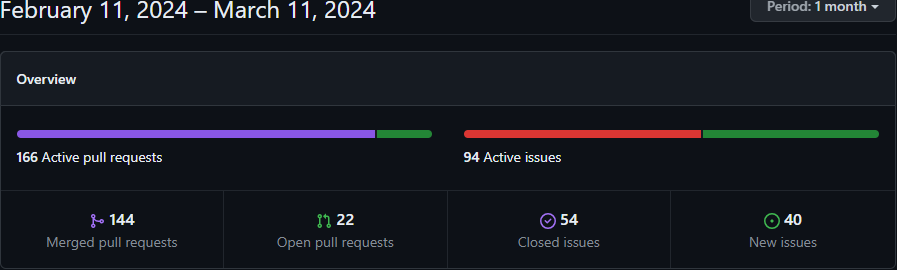
\includegraphics[width=0.75\linewidth]{source/implementation/evaluation/postgresql_ha_solutions/insights/cloudnativepg/pulse_cloudnative-pg_cloudnative-pg}
        \caption{CloudNativePG - Pulse}
        \label{fig:pulse_cloudnative-pg_cloudnative-pg}
    \end{figure}

    Der Code ist aber gut gepflegt, Code wird nicht nur regelmässig hinzugefügt, sondern auch entfernt.
    Auffällig ist, dass im April 2022 eine grosse Menge Code entfernt wurde:
    \begin{figure}[H]
        \centering
        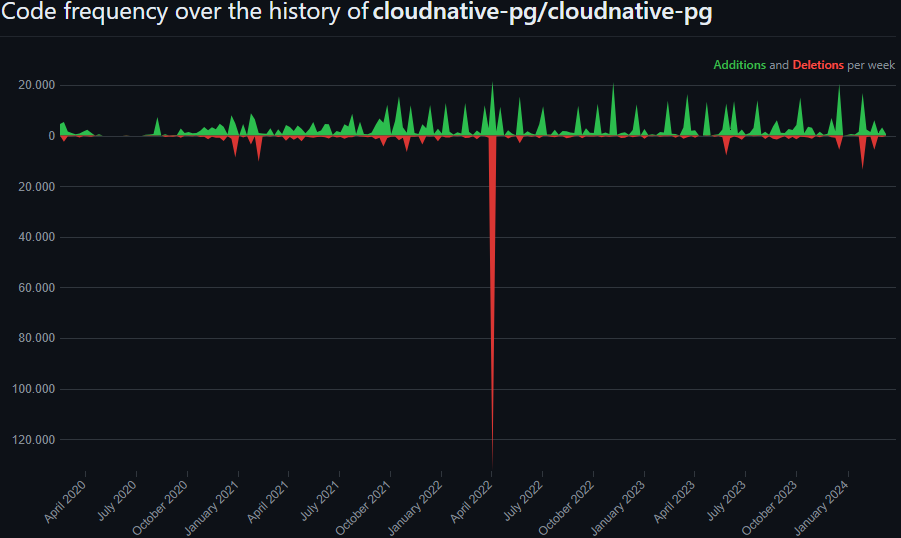
\includegraphics[width=0.75\linewidth]{source/implementation/evaluation/postgresql_ha_solutions/insights/cloudnativepg/code_frequency_cloudnative-pg_cloudnative-pg}
        \caption{CloudNativePG - Code Frequency}
        \label{fig:code_frequency_cloudnative-pg_cloudnative-pg}
    \end{figure}

    Das Projekt hält die meisten Standards von GitHub ein:
    \begin{figure}[H]
        \centering
        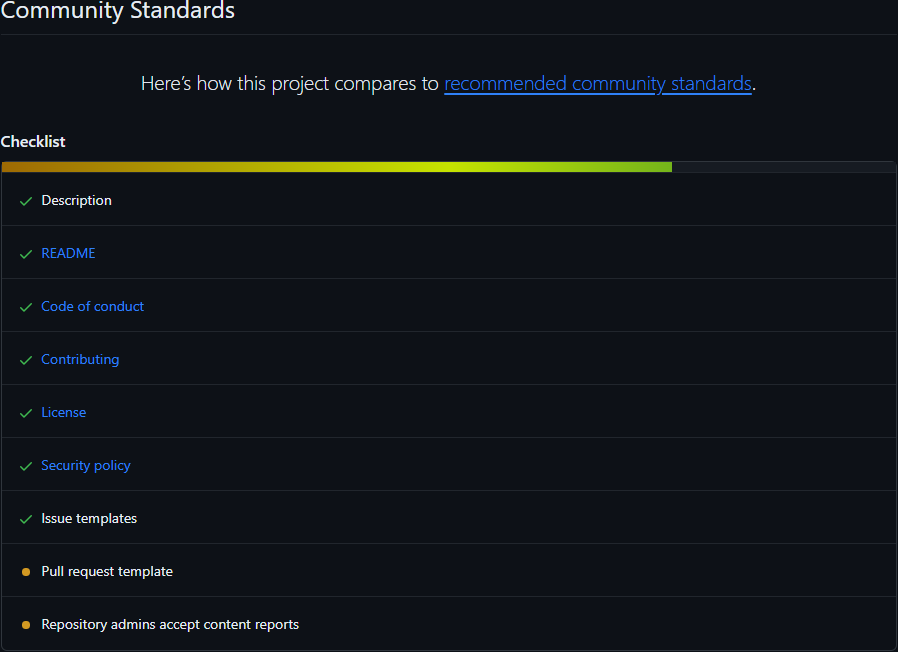
\includegraphics[width=0.75\linewidth]{source/implementation/evaluation/postgresql_ha_solutions/insights/cloudnativepg/community_standards}
        \caption{CloudNativePG - Community Standards}
        \label{fig:community_standards_cloudnativepg}
    \end{figure}
    Die Contributors committen zwar regelmässig auf das Projekt, allerdings fügen sie ungleich mehr dazu, als sie alten Code bereinigen.\\
    Das führt dann dazu, dass es zu grösseren Aufräumarbeiten kommt wie im April 2022.\\
    Es kann der Eindruck gewonnen werden, dass der Code wenig aufgeräumt wird und viel Ballast mit sich schleppt,\\
    was ein Sicherheitsrisiko darstellen kann:
    \begin{figure}[H]
        \centering
        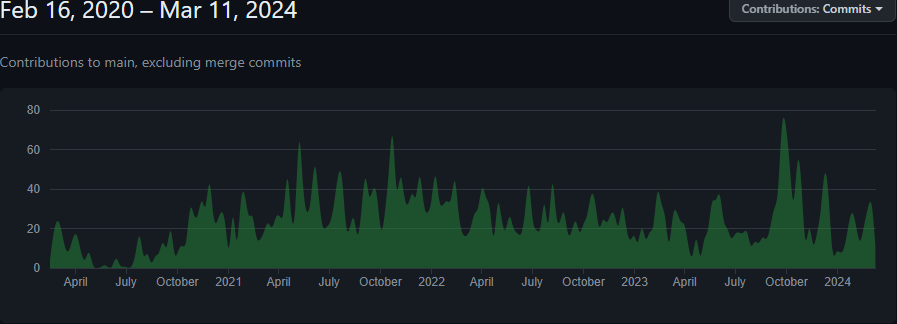
\includegraphics[width=0.75\linewidth]{source/implementation/evaluation/postgresql_ha_solutions/insights/cloudnativepg/contributors_commits_cloudnative-pg_cloudnative-pg}
        \caption{CloudNativePG - Contributors Commits}
        \label{fig:contributors_commits_cloudnative-pg_cloudnative-pg}
    \end{figure}
    \begin{figure}[H]
        \centering
        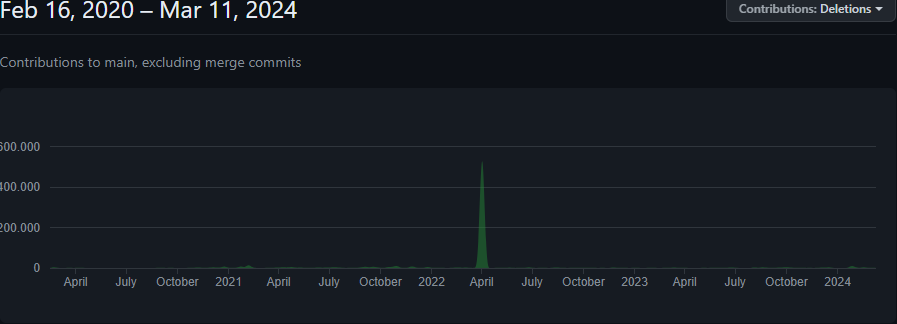
\includegraphics[width=0.75\linewidth]{source/implementation/evaluation/postgresql_ha_solutions/insights/cloudnativepg/contributors_deletations_cloudnative-pg_cloudnative-pg}
        \caption{CloudNativePG - Contributors Deletations}
        \label{fig:contributors_deletations_cloudnative-pg_cloudnative-pg}
    \end{figure}
    \begin{figure}[H]
        \centering
        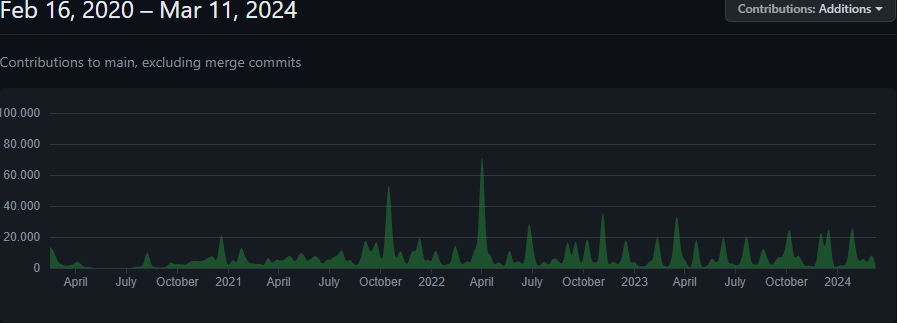
\includegraphics[width=0.75\linewidth]{source/implementation/evaluation/postgresql_ha_solutions/insights/cloudnativepg/contributors_additions_cloudnative-pg_cloudnative-pg}
        \caption{CloudNativePG - Contributors Additions}
        \label{fig:contributors_additions_cloudnative-pg_cloudnative-pg}
    \end{figure}
    Commits werden regelmässig abgesetzt, allerdings gibt es immer wieder gehäufte Commits.\\
    Oft um die Monatswechsel herum:
    \begin{figure}[H]
        \centering
        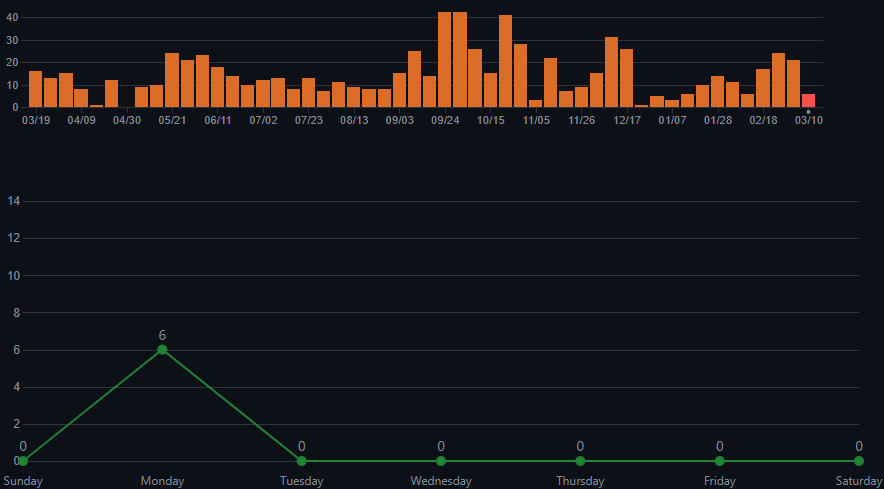
\includegraphics[width=0.75\linewidth]{source/implementation/evaluation/postgresql_ha_solutions/insights/cloudnativepg/commit_activity_cloudnative-pg_cloudnative-pg}
        \caption{CloudNativePG - Commit Activity}
        \label{fig:commit_activity_cloudnative-pg_cloudnative-pg}
    \end{figure}
    Nebst dem Projekt cloudnative-pg der \guillemotleft© The CloudNativePG Contributors\guillemotright ist CloudNativePG-Gründer EDB noch immer ein grosser Contributor.
     \begin{figure}[H]
        \centering
        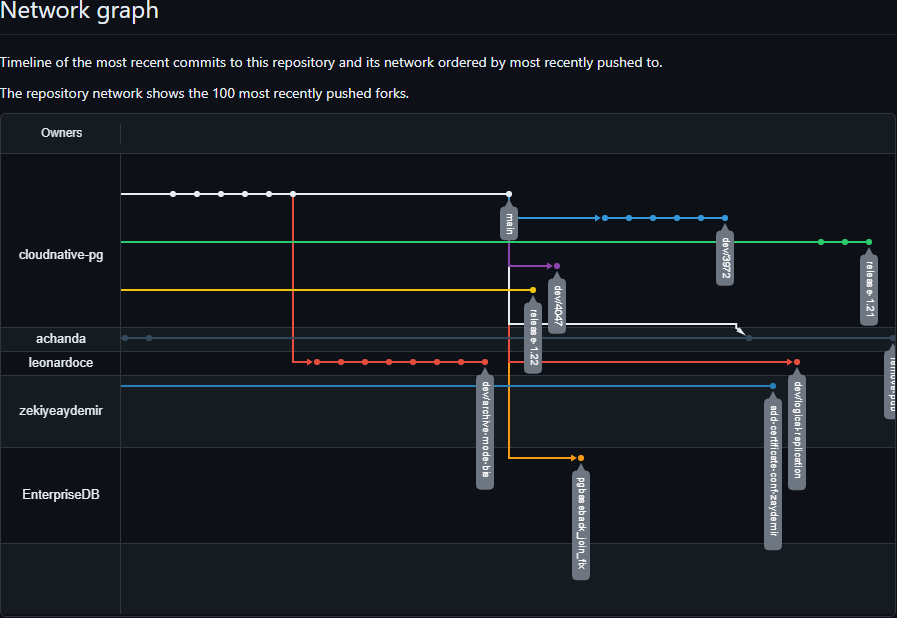
\includegraphics[width=0.75\linewidth]{source/implementation/evaluation/postgresql_ha_solutions/insights/cloudnativepg/network_graph_cloudnative-pg_cloudnative-pg}
        \caption{CloudNativePG - Network Graph}
        \label{fig:network_graph_cloudnative-pg_cloudnative-pg}
    \end{figure}
\end{flushleft}
    %! Author = gramic
%! Date = 21.04.24

% Preamble
\begin{flushleft}
    \subsection{Maintenance - Patroni}
    \label{subsec:maintenance_patroni}
    Patroni wird von Zalando regelmässig gepflegt.
    Das Projekt hat eine überschaubare Anzahl an Issues, wird aber Regelmässig
    \begin{figure}[H]
        \centering
        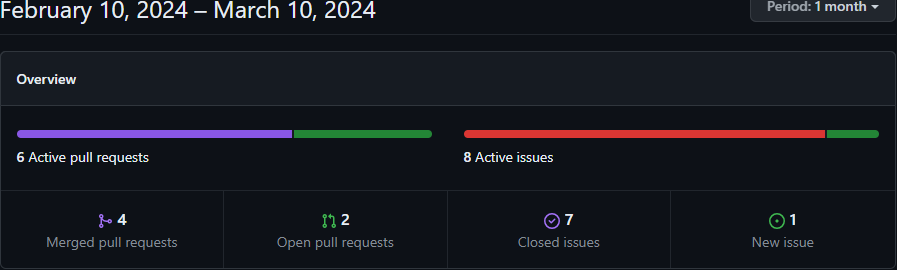
\includegraphics[width=0.75\linewidth]{source/implementation/evaluation/postgresql_ha_solutions/insights/patroni/pulse_zalando_patroni}
        \caption{Patroni - Pulse}
        \label{fig:pulse_zalando_patroni}
    \end{figure}

    Code wird Regelmässig hinzugefügt und entfernt:
    \begin{figure}[H]
        \centering
        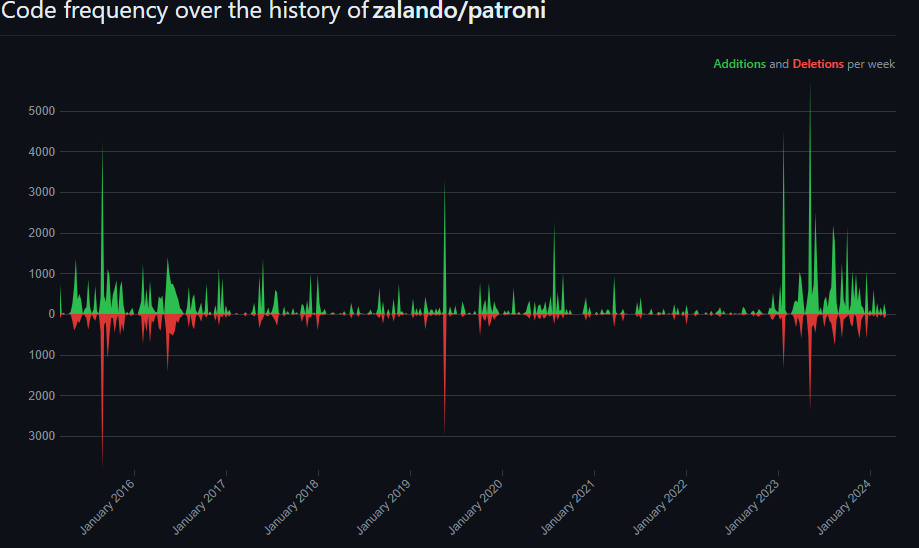
\includegraphics[width=0.75\linewidth]{source/implementation/evaluation/postgresql_ha_solutions/insights/patroni/code_frequency_zalando_patroni}
        \caption{Patroni - Code Frequency}
        \label{fig:code_frequency_zalando_patroni}
    \end{figure}
    Das Projekt hält auch die gängigen Standards auf Github ein:
    \begin{figure}[H]
        \centering
        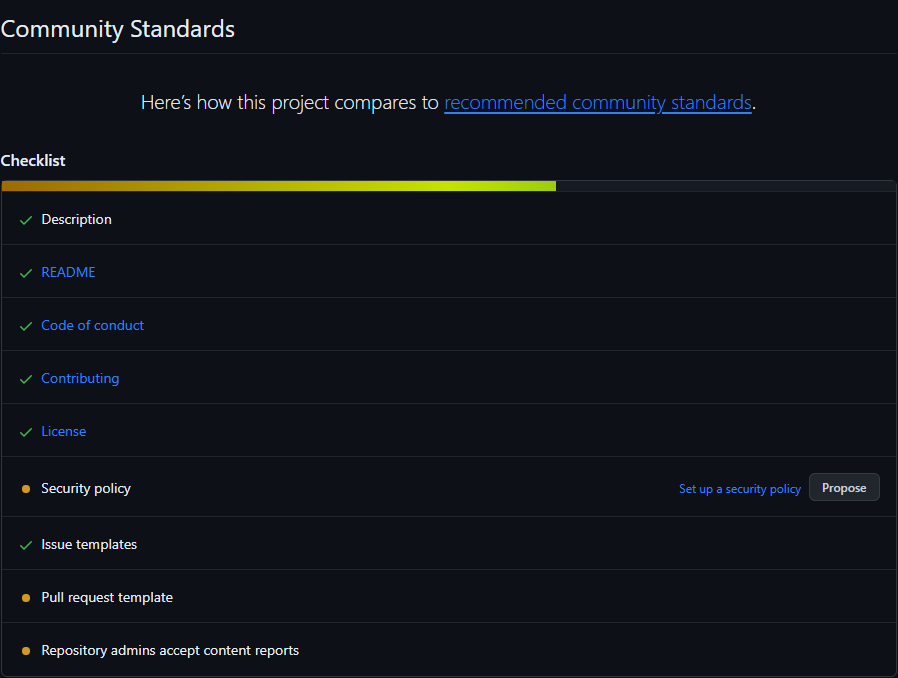
\includegraphics[width=0.75\linewidth]{source/implementation/evaluation/postgresql_ha_solutions/insights/patroni/community_Standards_zalando_patroni}
        \caption{Patroni - Community Standards}
        \label{fig:community_Standards_zalando_patroni}
    \end{figure}

    Die Contributors commiten, löschen und erweitern Patroni Regelmässig:
    \begin{figure}[H]
        \centering
        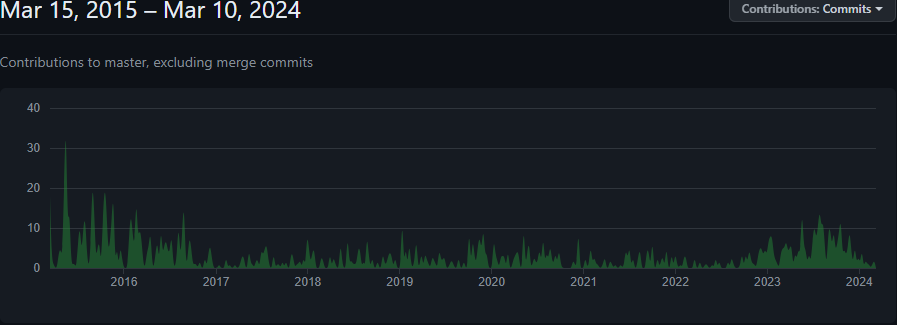
\includegraphics[width=0.75\linewidth]{source/implementation/evaluation/postgresql_ha_solutions/insights/patroni/contributors_commits_zalando_patroni}
        \caption{Patroni - Contributors Commits}
        \label{fig:contributors_commits_zalando_patroni}
    \end{figure}
    \begin{figure}[H]
        \centering
        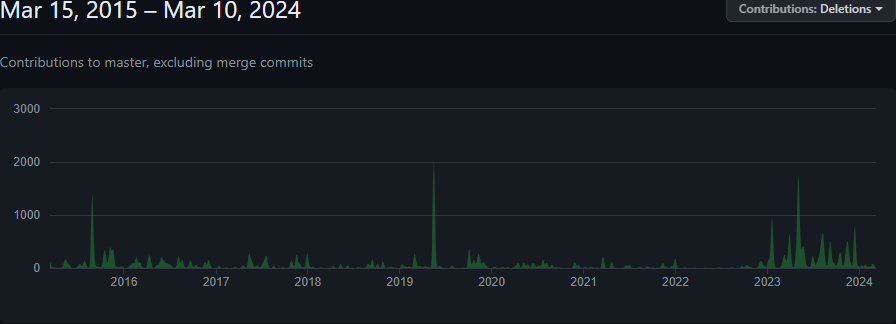
\includegraphics[width=0.75\linewidth]{source/implementation/evaluation/postgresql_ha_solutions/insights/patroni/contributors_deletations_zalando_patroni}
        \caption{Patroni - Contributors Deletations}
        \label{fig:contributors_deletations_zalando_patroni}
    \end{figure}
    \begin{figure}[H]
        \centering
        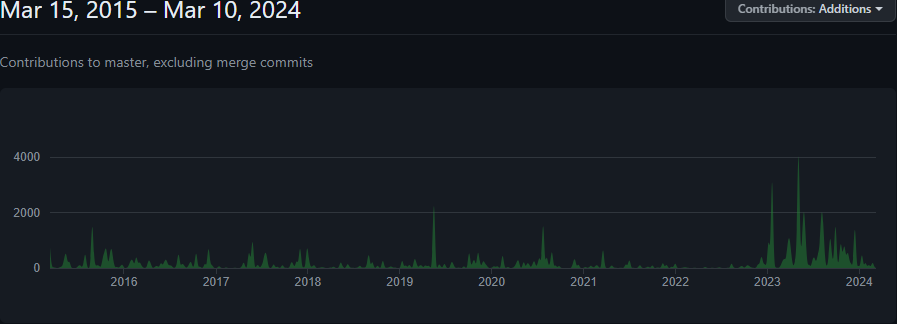
\includegraphics[width=0.75\linewidth]{source/implementation/evaluation/postgresql_ha_solutions/insights/patroni/contributors_additions_zalando_patroni}
        \caption{Patroni - Contributors Additions}
        \label{fig:contributors_additions_zalando_patroni}
    \end{figure}

    Commits werden nach wie vor immer noch Regelmässig eingespielt, auch wenn die Frequenz etwas nachgelassen hat:
    \begin{figure}[H]
        \centering
        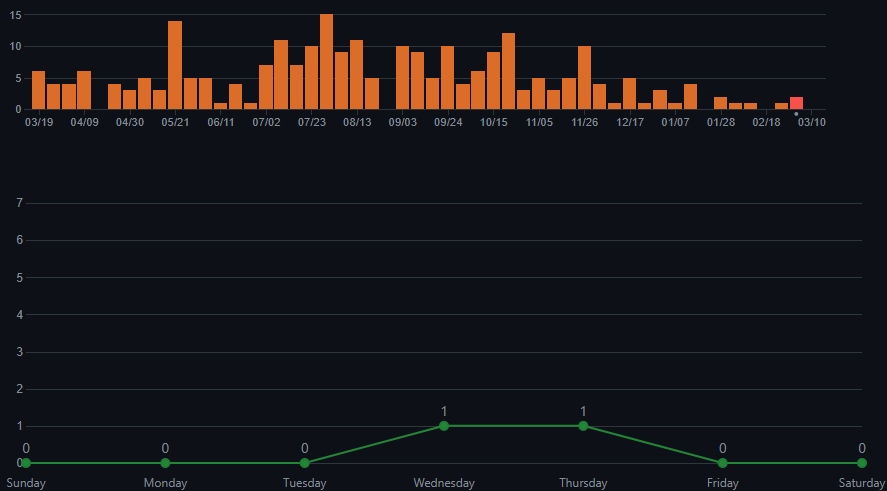
\includegraphics[width=0.75\linewidth]{source/implementation/evaluation/postgresql_ha_solutions/insights/patroni/commit_activity_zalando_patroni}
        \caption{Patroni - Commit Activity}
        \label{fig:commit_activity_zalando_patroni}
    \end{figure}

    Nebst Zalando selbst hat auch EnterpriseDB\cite{LNF967SI} ein grösseres Repository eingebunden.
    Dies weil EnterpriseDB stark auf Patroni setzt.
     \begin{figure}[H]
        \centering
        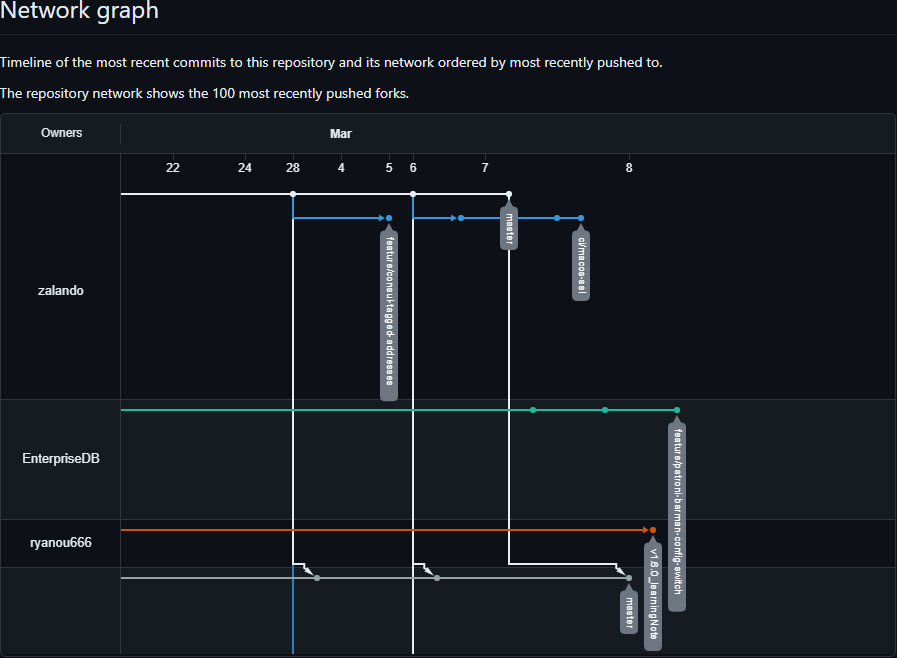
\includegraphics[width=0.75\linewidth]{source/implementation/evaluation/postgresql_ha_solutions/insights/patroni/networkgraph_zalando_patroni}
        \caption{Patroni - Network Graph}
        \label{fig:networkgraph_zalando_patroni}
    \end{figure}
\end{flushleft}
    %! Author = gramic
%! Date = 21.04.24

% Preamble
\begin{flushleft}
    \subsection{Maintenance - StackGres - Citus}
    \label{subsec:maintenance_stackgres_citus}
    Bei StackGres gab es im letzten Monat keine wirkliche Bewegung:
    \begin{figure}[H]
        \centering
        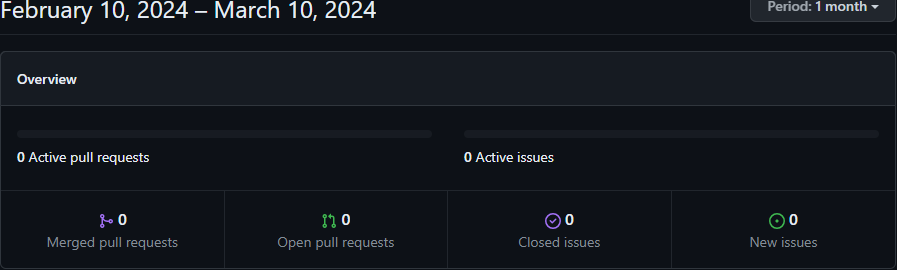
\includegraphics[width=0.75\linewidth]{source/implementation/evaluation/postgresql_ha_solutions/insights/stackgres_citus/pulse_ongres_stackgres}
        \caption{Stackgres - Pulse}
        \label{fig:pulse_ongres_stackgres}
    \end{figure}
    Anders sieht es bei Citus aus, die Firma, die mittlerweile zu Microsoft gehört, schliesst Issues rasch und hat eine verhältnismässig hohe Requstrate:
    \begin{figure}[H]
        \centering
        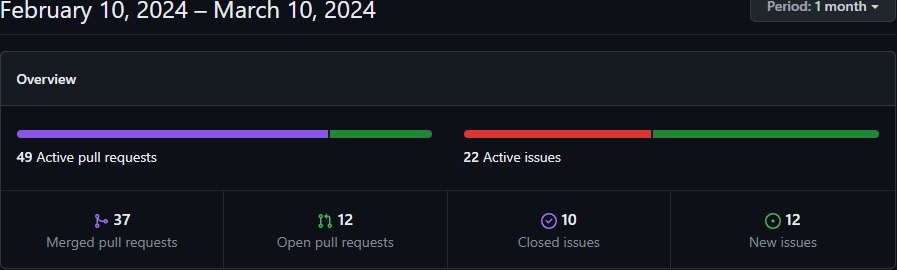
\includegraphics[width=0.75\linewidth]{source/implementation/evaluation/postgresql_ha_solutions/insights/stackgres_citus/pulse_citusdata_citus}
        \caption{Citus - Pulse}
        \label{fig:pulse_citusdata_citus}
    \end{figure}
    Bei StackGres wird sehr viel Code hinzugefügt oder gelöscht, beim älteren Citus wurden weniger Änderungen verzeichnet:
    \begin{figure}[H]
        \centering
        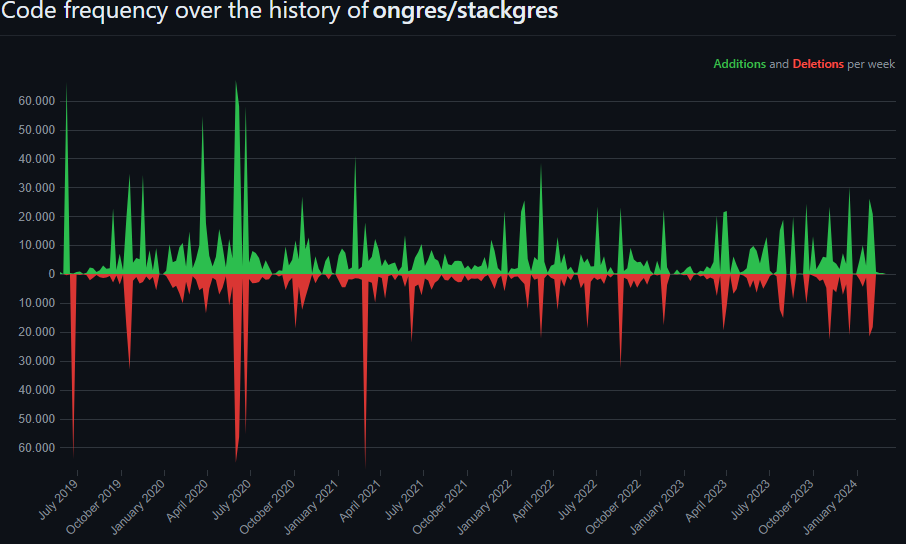
\includegraphics[width=0.75\linewidth]{source/implementation/evaluation/postgresql_ha_solutions/insights/stackgres_citus/code_frequency_ongres_stackgres}
        \caption{Stackgres - Code Frequency}
        \label{fig:code_frequency_ongres_stackgres}
    \end{figure}
    \begin{figure}[H]
        \centering
        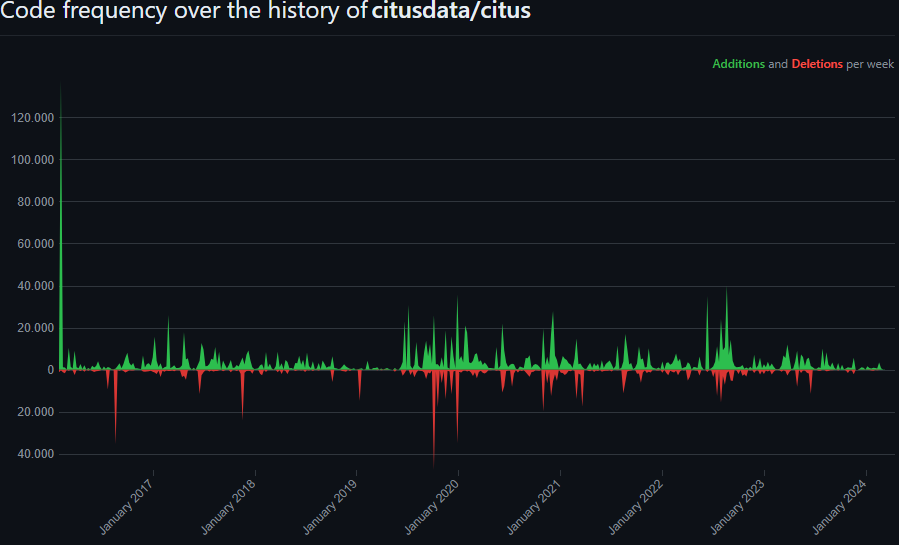
\includegraphics[width=0.75\linewidth]{source/implementation/evaluation/postgresql_ha_solutions/insights/stackgres_citus/code_frequency_citusdata_citus}
        \caption{Citus - Code Frequency}
        \label{fig:code_frequency_citusdata_citus}
    \end{figure}
    Citus legt einen hohen Stellenwert auf die Community-Standars, StackGres selbst schneidet hier nur mittelmässig ab:
    \begin{figure}[H]
        \centering
        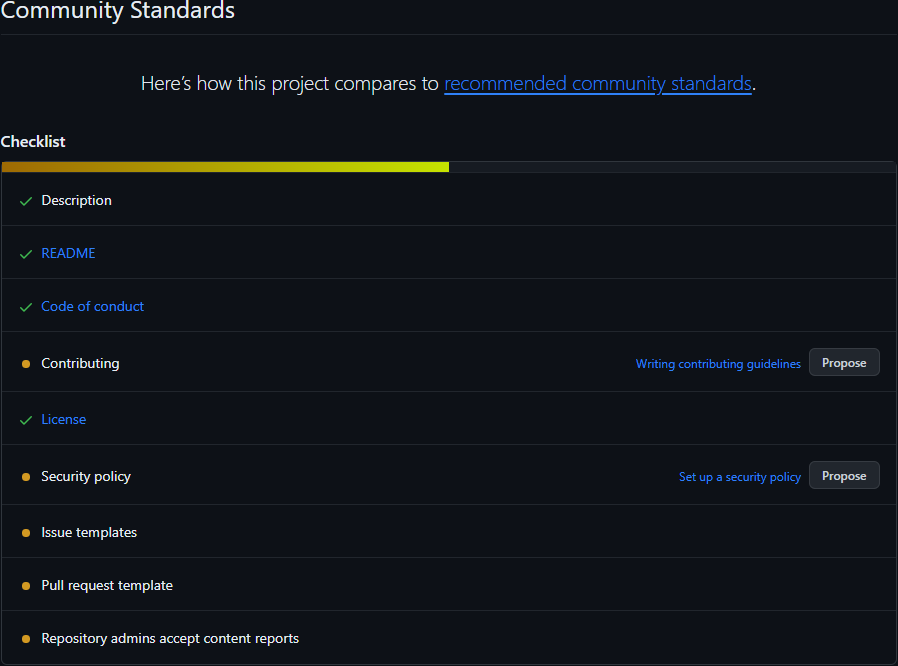
\includegraphics[width=0.75\linewidth]{source/implementation/evaluation/postgresql_ha_solutions/insights/stackgres_citus/stackgres_community_standards}
        \caption{Stackgres - Community Standards}
        \label{fig:stackgres_community_standards}
    \end{figure}
    \begin{figure}[H]
        \centering
        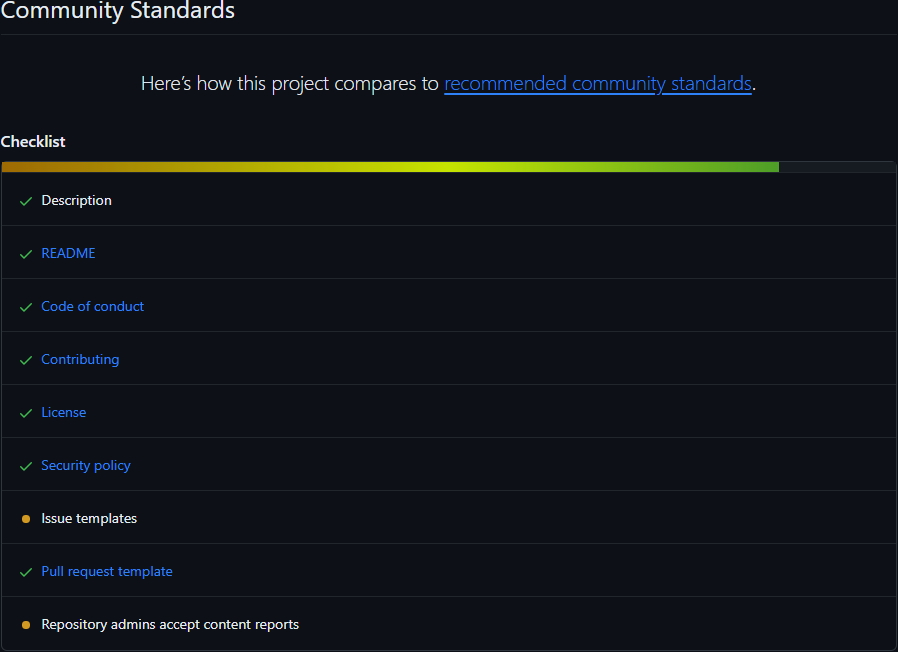
\includegraphics[width=0.75\linewidth]{source/implementation/evaluation/postgresql_ha_solutions/insights/stackgres_citus/citus_community_standards}
        \caption{Citus - Community Standards}
        \label{fig:citus_community_standards}
    \end{figure}

    Die Stackgres Constributors pflegen aktiv Additions ein, löschen regelmässig und Commiten ebenfalls auf die main-Branch.
    Citus, dessen Repository länger Commited wird, hat weniger Bewegung auf die main-Branch.
    \begin{figure}[H]
        \centering
        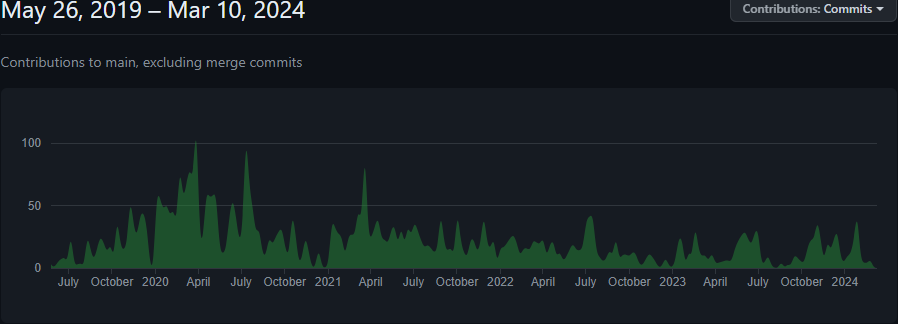
\includegraphics[width=0.75\linewidth]{source/implementation/evaluation/postgresql_ha_solutions/insights/stackgres_citus/contributors_commits_ongres_stackgres}
        \caption{Stackgres - Contributors Commits}
        \label{fig:contributors_commits_ongres_stackgres}
    \end{figure}
    \begin{figure}[H]
        \centering
        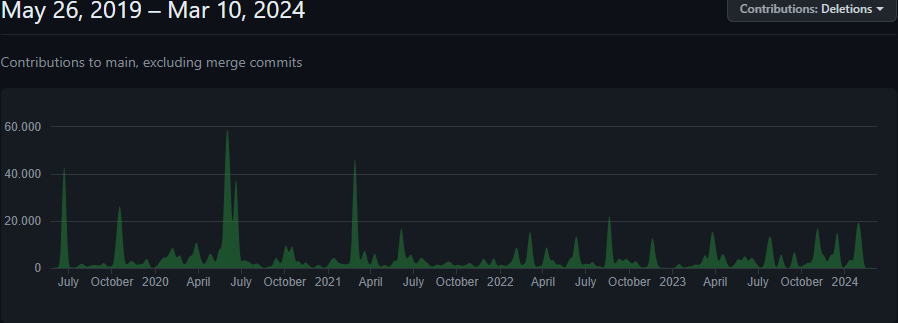
\includegraphics[width=0.75\linewidth]{source/implementation/evaluation/postgresql_ha_solutions/insights/stackgres_citus/contributors_deletations_ongres_stackgres}
        \caption{Stackgres - Contributors Deletations}
        \label{fig:contributors_deletations_ongres_stackgres}
    \end{figure}
    \begin{figure}[H]
        \centering
        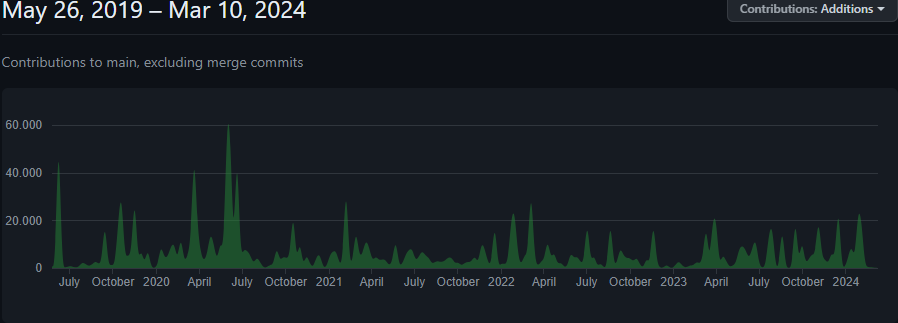
\includegraphics[width=0.75\linewidth]{source/implementation/evaluation/postgresql_ha_solutions/insights/stackgres_citus/contributors_addition_ongres_stackgres}
        \caption{Stackgres - Contributors Additions}
        \label{fig:contributors_addition_ongres_stackgres}
    \end{figure}
    \begin{figure}[H]
        \centering
        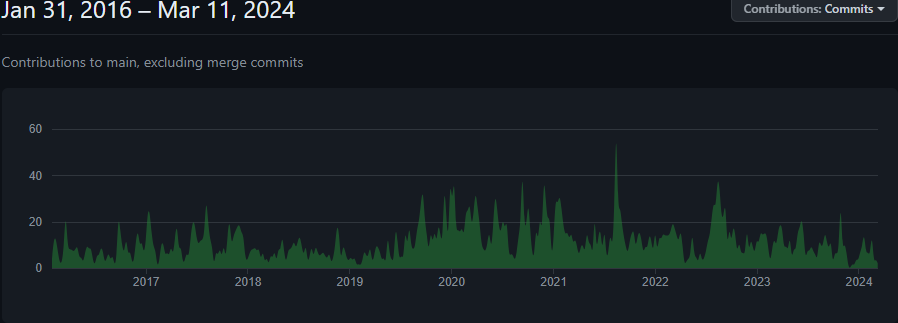
\includegraphics[width=0.75\linewidth]{source/implementation/evaluation/postgresql_ha_solutions/insights/stackgres_citus/contributors_commits_citusdata_citus}
        \caption{Citus - Contributors Commits}
        \label{fig:contributors_commits_citusdata_citus}
    \end{figure}
    \begin{figure}[H]
        \centering
        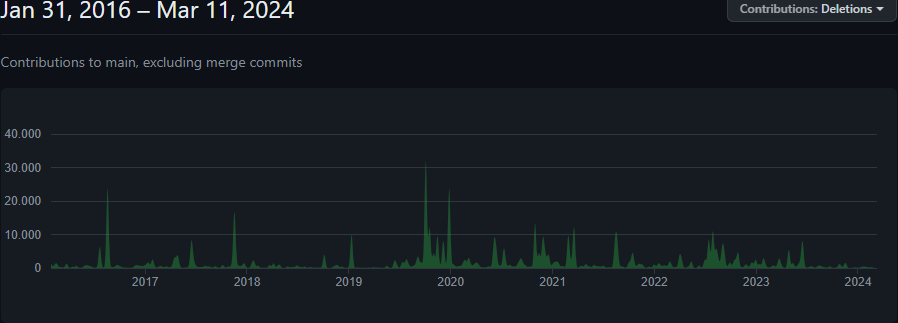
\includegraphics[width=0.75\linewidth]{source/implementation/evaluation/postgresql_ha_solutions/insights/stackgres_citus/contributors_deletations_citusdata_citus}
        \caption{Citus - Contributors Deletations}
        \label{fig:contributors_deletations_citusdata_citus}
    \end{figure}
    \begin{figure}[H]
        \centering
        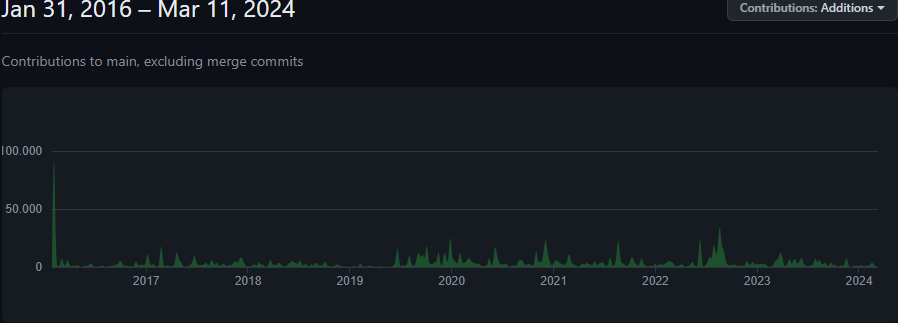
\includegraphics[width=0.75\linewidth]{source/implementation/evaluation/postgresql_ha_solutions/insights/stackgres_citus/contributors_additions_citusdata_citus}
        \caption{Citus - Contributors Additions}
        \label{fig:contributors_additions_citusdata_citus}
    \end{figure}
    Gerade Ende Januar gab es bei StackGres eine grössere Anzahl Commits, anhand der Statistik wird ersichtlich, dass i. d. R. einmal pro Monat grössere Mengen an Commits eingespielt werden.
    Bei Citus gibt es ebenfalls regelmässig grössere Mengen an Commits, allerdings scheint bei citusdata mehr mit kürzeren Sprints gearbeitet zu werden als bei Ongres denn die Commits sind regelmässiger:
    \begin{figure}[H]
        \centering
        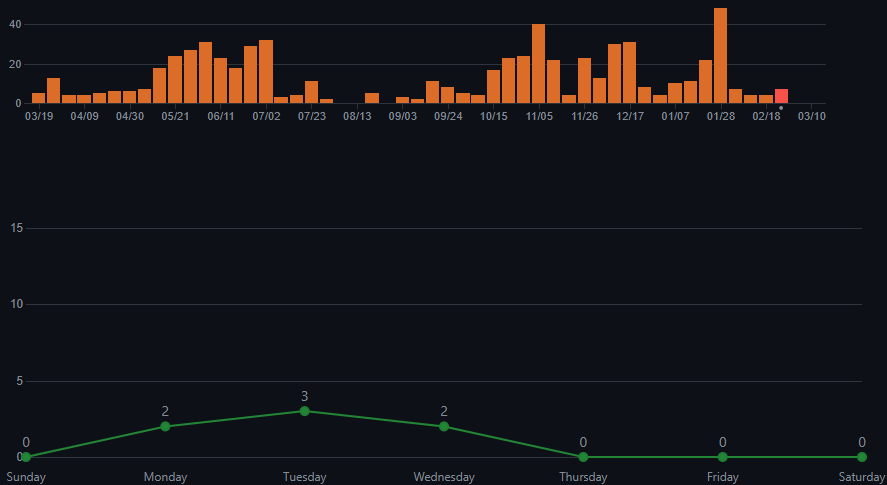
\includegraphics[width=0.75\linewidth]{source/implementation/evaluation/postgresql_ha_solutions/insights/stackgres_citus/commit_activity_ongres_stackgres}
        \caption{Stackgres - Commit Activity}
        \label{fig:commit_activity_ongres_stackgres}
    \end{figure}
    \begin{figure}[H]
        \centering
        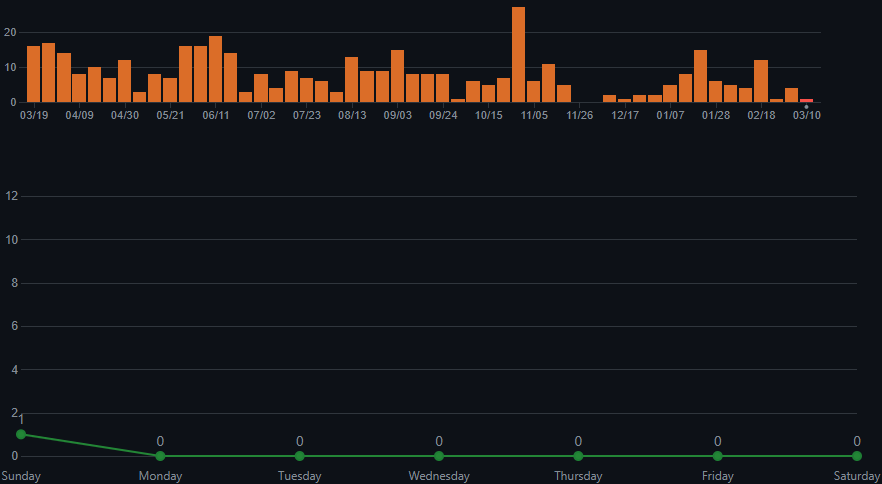
\includegraphics[width=0.75\linewidth]{source/implementation/evaluation/postgresql_ha_solutions/insights/stackgres_citus/commit_activity_citusdata_citus}
        \caption{Citus - Commit Activity}
        \label{fig:commit_activity_citusdata_citus}
    \end{figure}
    In letzter Zeit haben nur Ongres, der Entwickler von StackGres, als auch citusdata, grössere Commits auf das Repository gefahren.
    Andere grössere Entwickler wie EnterpriseDB sind abwesend.
    \begin{figure}[H]
        \centering
        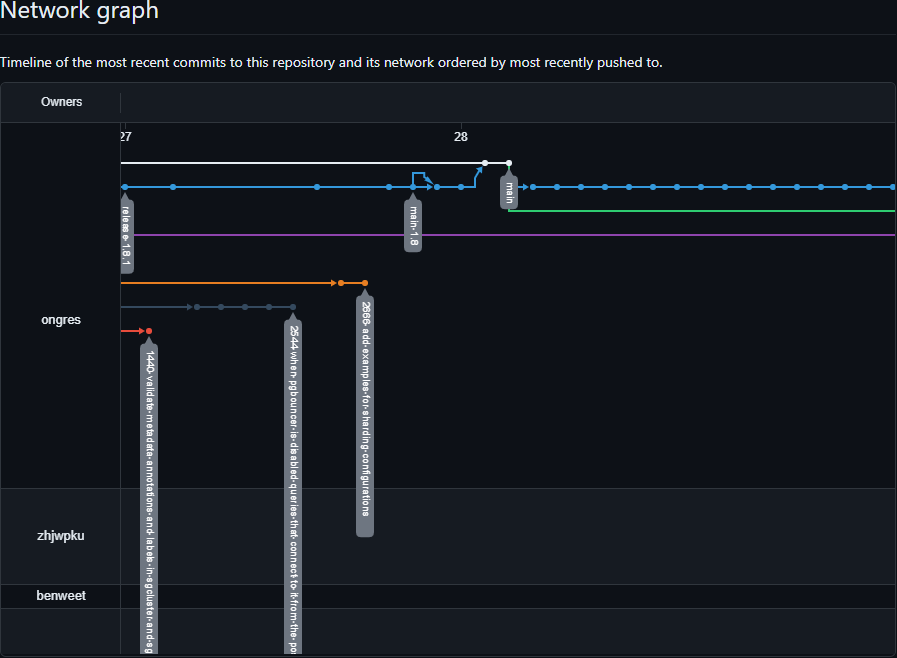
\includegraphics[width=0.75\linewidth]{source/implementation/evaluation/postgresql_ha_solutions/insights/stackgres_citus/network_graph_ongres_stackgres}
        \caption{Stackgres - Network Graph}
        \label{fig:network_graph_ongres_stackgres}
    \end{figure}
    \begin{figure}[H]
        \centering
        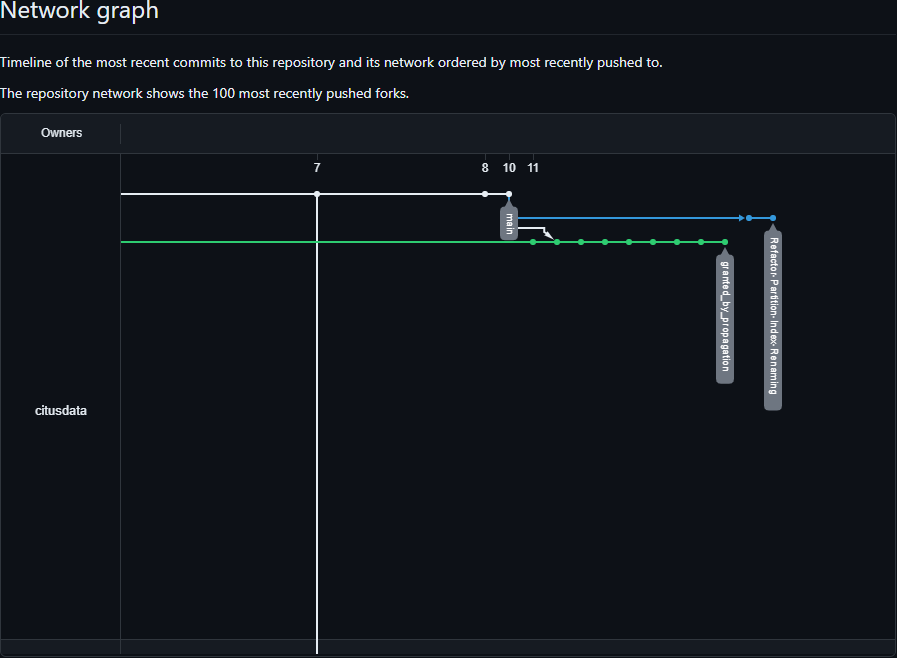
\includegraphics[width=0.75\linewidth]{source/implementation/evaluation/postgresql_ha_solutions/insights/stackgres_citus/network_graph_citusdata_citus}
        \caption{Citus - Network Graph}
        \label{fig:network_graph_citusdata_citus}
    \end{figure}
\end{flushleft}
    %! Author = gramic
%! Date = 21.04.24

% Preamble
\clearpage
\KOMAoptions{paper=A4,paper=portrait,pagesize}
\recalctypearea
\begin{flushleft}
%    \clearpage
%    \KOMAoptions{paper=A4,paper=portrait,pagesize}
%    \recalctypearea
    \subsection{Maintenance - YugabyteDB}
    \label{subsec:maintenance_yugabytedb}
    Das Projekt hat eine sehr hohe Anzahl an aktiven Issues, wobei viele neue dazugekommen sind:
    \begin{figure}[H]
        \centering
        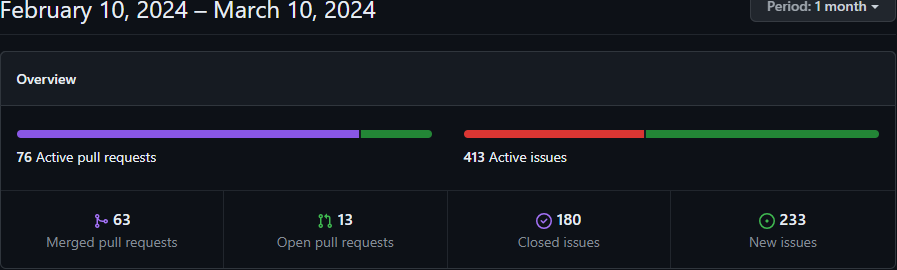
\includegraphics[width=0.75\linewidth]{source/implementation/evaluation/postgresql_ha_solutions/insights/yugabytedb/pulse_yugabyte_yugabyte-db}
        \caption{YugabyteDB - Pulse}
        \label{fig:pulse_yugabyte_yugabyte-db}
    \end{figure}

    Die Code Frequency kann nicht ausgegeben werden, es gab zu viele Commits:
    \begin{figure}[H]
        \centering
        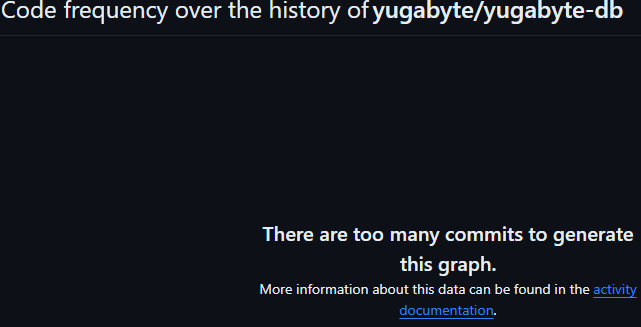
\includegraphics[width=0.75\linewidth]{source/implementation/evaluation/postgresql_ha_solutions/insights/yugabytedb/code_frequency_yugabyte_yugabyte-db}
        \caption{YugabyteDB - Code Frequency}
        \label{fig:code_frequency_yugabyte_yugabyte-db}
    \end{figure}

    Das Projekt hält nur die wichtigsten Community Standards ein:
    \begin{figure}[H]
        \centering
        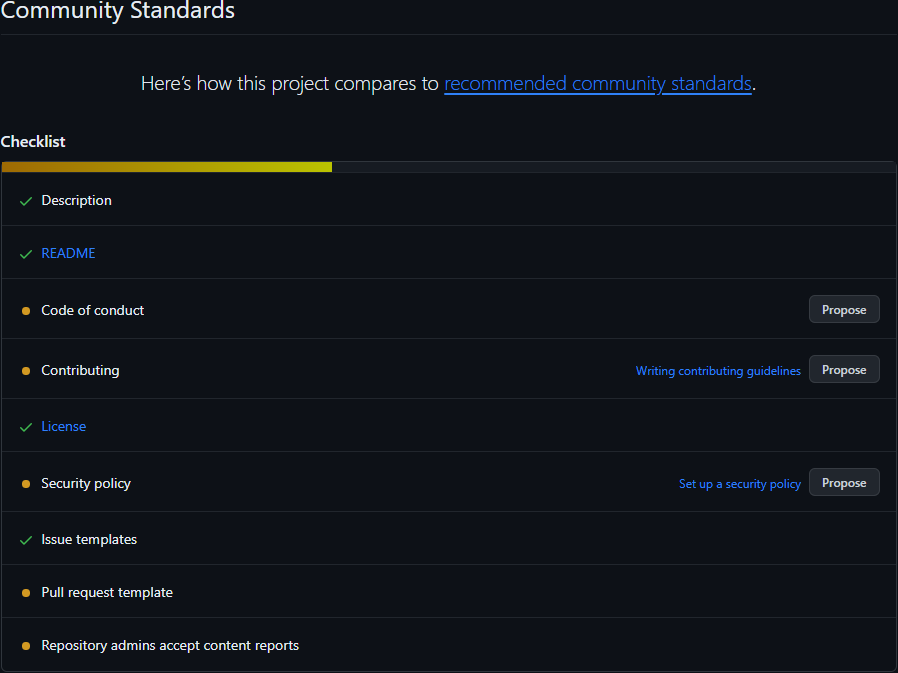
\includegraphics[width=0.75\linewidth]{source/implementation/evaluation/postgresql_ha_solutions/insights/yugabytedb/community Standards}
        \caption{YugabyteDB - Community Standards}
        \label{fig:community Standards_yugabyte-db}
    \end{figure}

    Es werden immer wieder Commits abgesetzt, allerdings sind diese nicht weiter aufgeteilt in Commits, Additions und Deletations:
    \begin{figure}[H]
        \centering
        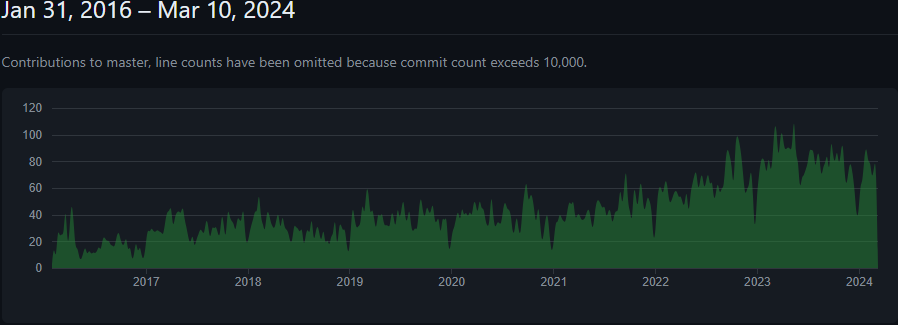
\includegraphics[width=0.75\linewidth]{source/implementation/evaluation/postgresql_ha_solutions/insights/yugabytedb/contributors_to_yugabyte_yugabyte-db}
        \caption{YugabyteDB - Contributors}
        \label{fig:contributors_to_yugabyte_yugabyte-db}
    \end{figure}
\end{flushleft}
\clearpage
\KOMAoptions{paper=A4,paper=portrait,pagesize}
\recalctypearea
\begin{flushleft}
    Die Commits wiederum werden regelmässig ausgeführt, es wird scheinbar in kurzen Sprints gearbeitet:
    \begin{figure}[H]
        \centering
        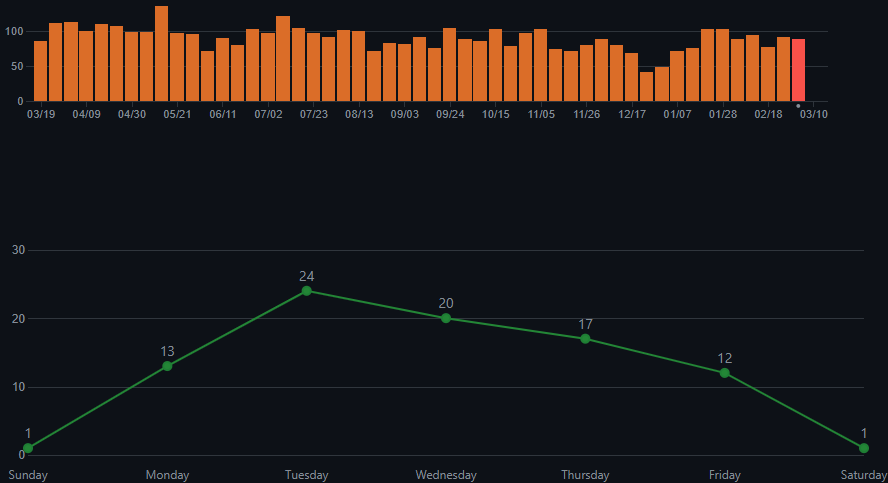
\includegraphics[width=0.75\linewidth]{source/implementation/evaluation/postgresql_ha_solutions/insights/yugabytedb/commit_activity_yugabyte_yugabyte-db}
        \caption{YugabyteDB - Commit Activity}
        \label{fig:commit_activity_yugabyte_yugabyte-db}
    \end{figure}
    YugabyteDB ist der Maintainer seines Produkts.\\
    Es gibt keine anderen grossen Contributors:
     \begin{figure}[H]
        \centering
        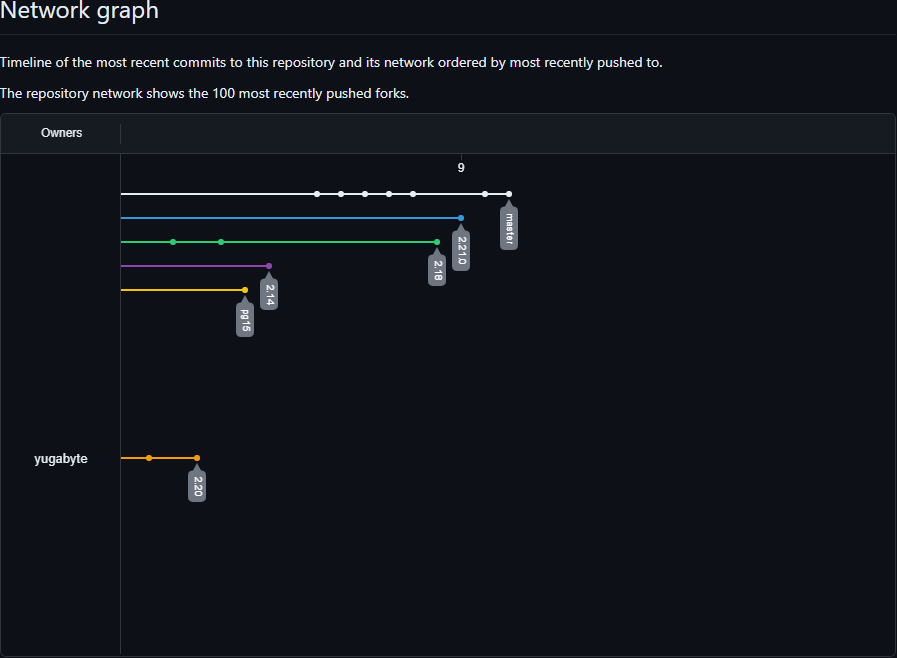
\includegraphics[width=0.75\linewidth]{source/implementation/evaluation/postgresql_ha_solutions/insights/yugabytedb/network_graph_yugabyte_yugabyte-db}
        \caption{YugabyteDB - Network Graph}
        \label{fig:network_graph_yugabyte_yugabyte-db}
    \end{figure}
\end{flushleft}
\end{flushleft}
    %! Author = gramic
%! Date = 21.04.24

% Preamble
\begin{flushleft}
    \section{Evaluationssysteme - Installation}
    %! Author = itgramic
%! Date = 26.01.24

% Preamble
\section{rke2}
\subsection{Vorbereitung}
Da Package aus WAN-Repositories geladen werden, muss eine Proxy-Connection nach aussen gemacht werden können:
\lstset{style=gra_codestyle}
\begin{lstlisting}[language=bash, caption=Proxy Settings,captionpos=b,label={lst:proxy-settings},breaklines=true]
sudo nano /etc/profile.d/proxy.sh

export https_proxy=http://sproxy.sivc.first-it.ch:8080
export HTTPS_PROXY=http://sproxy.sivc.first-it.ch:8080
export http_proxy=http://sproxy.sivc.first-it.ch:8080
export HTTP_PROXY=http://sproxy.sivc.first-it.ch:8080
export no_proxy=localhost,127.0.0.0/8,::1,10.0.0.0/8,172.16.0.0/12,192.168.0.0/16
export NO_PROXY=localhost,127.0.0.0/8,::1,10.0.0.0/8,172.16.0.0/12,192.168.0.0/16

source /etc/profile.d/proxy.sh
\end{lstlisting}

\subsection{Installation}
\subsubsection{server - sks1183}
Es gibt kein apt-Package.
Daher muss zuerst das tarball-Package heruntergeladen werden.

Zuerst wird das Verzeichnis für rke2 erstellt:
\lstset{style=gra_codestyle}
\begin{lstlisting}[language=bash, caption=rke2 server - Verzeichnis erstellen,captionpos=b,label={lst:rke2-server-mkdir-rke2},breaklines=true]
mkdir -p /etc/rancher/rke2/
mkdir -p /var/lib/rancher/rke2/server/manifests/
\end{lstlisting}

\lstset{style=gra_codestyle}
\begin{lstlisting}[language=yaml, caption=rke2 server - config.yaml,captionpos=b,label={lst:rke2-server-config.yaml},breaklines=true]
# /etc/rancher/rke2/
cluster-cidr: "198.18.0.0/16"
service-cidr: "198.19.0.0/16"
cni:
  - cilium
disable:
  - rke2-canal
\end{lstlisting}

Cilium muss separat manifestiert werden:
\lstset{style=gra_codestyle}
\begin{lstlisting}[language=yaml, caption=rke2 server - cilium-config.yaml,captionpos=b,label={lst:rke2-server-cilium-config.yaml},breaklines=true]
# /var/lib/rancher/rke2/server/manifests/rke2-cilium-config.yaml
---
apiVersion: helm.cattle.io/v1
kind: HelmChartConfig
metadata:
  name: rke2-cilium
  namespace: kube-system
spec:
  valuesContent: |-
    eni:
      enabled: true
\end{lstlisting}

Das Package kann nun installiert und aktiviert werden:
\lstset{style=gra_codestyle}
\begin{lstlisting}[language=bash, caption=rke2 server installieren,captionpos=b,label={lst:install-rke2-server},breaklines=true]
curl -sfL https://get.rke2.io | INSTALL_RKE2_VERSION=v1.29.0+rke2r1 sh -
systemctl enable rke2-server.service
systemctl start rke2-server.service
\end{lstlisting}

\subsubsection{agents - sks1184 / sks1185}
Der Agent muss direkt heruntergeladen, installiert und aktiviert werden:
\lstset{style=gra_codestyle}
\begin{lstlisting}[language=bash, caption=rke2 agenten installieren,captionpos=b,label={lst:install-rke2-agent},breaklines=true]
curl -sfL https://get.rke2.io | INSTALL_RKE2_TYPE="agent" INSTALL_RKE2_VERSION=v1.29.0+rke2r1 sh -
systemctl enable rke2-agent.service
mkdir -p /etc/rancher/rke2/
\end{lstlisting}

Die Konfiguration muss nun konfiguriert werden.
Dem Agents müssen den Server und den Server Token erhalten:
\lstset{style=gra_codestyle}
\begin{lstlisting}[language=yaml, caption=rke2 agent - config.yaml,captionpos=b,label={lst:rke2-agent-config.yaml},breaklines=true]
# /etc/rancher/rke2/config.yaml
server: https://10.0.20.97:9345
token: K1042bf32f28282edad37cbac4b77ccfa1cd44a26f0ea2c19111ed664013954a326::server:7a430a28b29501b778543f0882a156b8
\end{lstlisting}

Nun muss der Dienst restartet werden
\lstset{style=gra_codestyle}
\begin{lstlisting}[language=bash, caption=-rke2 agent service restart,captionpos=b,label={lst:rke2-agent-service-restart},breaklines=true]
systemctl start rke2-agent.service
\end{lstlisting}

\subsection{Cluster Konfiguration}
\subsubsection{server}
Auch für Kubernetes und die Pots müssen die Proxy-Einstellungen gemacht werden:
\lstset{style=gra_codestyle}
\begin{lstlisting}[language=bash, caption=rke2 server proxy,captionpos=b,label={lst:rke2-server-proxy},breaklines=true]
nano /etc/default/rke2-server
HTTPS_PROXY=http://sproxy.sivc.first-it.ch:8080
HTTP_PROXY=http://sproxy.sivc.first-it.ch:8080
NO_PROXY=localhost,127.0.0.0/8,::1,10.0.0.0/8,172.16.0.0/12,192.168.0.0/16

CONTAINERD_HTTPS_PROXY=http://sproxy.sivc.first-it.ch:8080
CONTAINERD_HTTP_PROXY=http://sproxy.sivc.first-it.ch:8080
CONTAINERD_NO_PROXY=localhost,127.0.0.0/8,::1,10.0.0.0/8,172.16.0.0/12,192.168.0.0/16
\end{lstlisting}

Dieses File muss entsprechend in das Homeverzeichnis gespeichert werden:
\lstset{style=gra_codestyle}
\begin{lstlisting}[language=bash, caption=rke2 server proxy kopieren,captionpos=b,label={lst:rke2-server-proxy-copy},breaklines=true]

\end{lstlisting}

Für den Netzwerkteil muss nun Cilium installiert werden:
\lstset{style=gra_codestyle}
\begin{lstlisting}[language=bash, caption=rke2 server cilium installieren,captionpos=b,label={lst:rke2-server-cilium-install},breaklines=true]

\end{lstlisting}

Cilium muss nun aktiviert werden:
\begin{lstlisting}[language=bash, caption=rke2 server cilium aktivieren,captionpos=b,label={lst:rke2-server-cilium-apply},breaklines=true]

\end{lstlisting}

Der rke2-Server muss nun mit der entsprechenden Config gestartet werden, anschliessend muss Cilium noch in die Conig und diese mittels Service reboot aktiviert werden:
\lstset{style=gra_codestyle}
\begin{lstlisting}[language=bash, caption=rke2 server starten,captionpos=b,label={lst:rke2-server-start},breaklines=true]

\end{lstlisting}

Entsprechend muss die Firewall gesetzt werden:
\lstset{style=gra_codestyle}
\begin{lstlisting}[language=bash, caption=iptables entries server,captionpos=b,label={lst:iptables-server-entries},breaklines=true]
nano /etc/iptables/rules.v4

# Generated by iptables-save v1.8.9 (nf_tables)
*filter
:INPUT DROP [0:0]
:FORWARD ACCEPT [0:0]
:OUTPUT ACCEPT [0:0]
-A INPUT -m state --state RELATED,ESTABLISHED -j ACCEPT
-A INPUT -p udp -m udp --sport 53 -j ACCEPT
-A INPUT -p icmp -j ACCEPT
-A INPUT -i lo -j ACCEPT
-A INPUT -s 10.0.0.0/8 -p tcp -m tcp --dport 22 -j ACCEPT
-A INPUT -s 10.0.9.115/32 -p udp -m udp --dport 161 -m comment --comment "Allow SNMP for probe 10.0.9.115" -j ACCEPT
-A INPUT -s 10.0.9.76/32 -p udp -m udp --dport 161 -m comment --comment "Allow SNMP for probe 10.0.9.76" -j ACCEPT
-A INPUT -s 10.0.36.147/32 -p udp -m udp --dport 161 -m comment --comment "Allow SNMP for probe 10.0.36.147" -j ACCEPT
-A INPUT -s 10.0.9.35/32 -p udp -m udp --dport 161 -m comment --comment "Allow SNMP for probe 10.0.9.35" -j ACCEPT
-A INPUT -s 10.0.9.37/32 -p udp -m udp --dport 161 -m comment --comment "Allow SNMP for probe 10.0.9.37" -j ACCEPT
-A INPUT -s 10.0.9.74/32 -p udp -m udp --dport 161 -m comment --comment "Allow SNMP for probe 10.0.9.74" -j ACCEPT
-A INPUT -s 10.0.9.75/32 -p udp -m udp --dport 161 -m comment --comment "Allow SNMP for probe 10.0.9.75" -j ACCEPT
-A INPUT -s 10.0.9.36/32 -p udp -m udp --dport 161 -m comment --comment "Allow SNMP for probe 10.0.9.36" -j ACCEPT
-A INPUT -s 10.0.9.14/32 -p udp -m udp --dport 161 -m comment --comment "Allow SNMP for probe 10.0.9.14" -j ACCEPT
-A INPUT -s 10.0.0.0/8 -p icmp -m icmp --icmp-type 8 -j ACCEPT
-A INPUT -s 10.0.0.0/8 -p tcp -m tcp --dport 6443 -j ACCEPT
-A INPUT -s 10.0.0.0/8 -p tcp -m tcp --dport 9345 -j ACCEPT
COMMIT
# Completed

systemctl restart iptables
\end{lstlisting}

Für den Connect der Agents muss noch ein Token generiert werden:
\begin{lstlisting}[language=bash, caption=rke2 server token,captionpos=b,label={lst:rke2-server-token},breaklines=true]
\end{lstlisting}

\subsubsection{agents}

\subsubsection{local-path-provisioner}
Zuerst mussten auf den drei Servern der Storage bereitgestellt werden:
\lstset{style=gra_codestyle}
\begin{lstlisting}[language=bash, caption=local-path-storage auf Linux Bereitstellen,captionpos=b,label={lst:local-path-storage-provide},breaklines=true]
root@sks1183:~# mkdir /var/local-path-provisioner
root@sks1183:~# chmod -R 777 /var/local-path-provisioner/

root@sks1184:~# mkdir /var/local-path-provisioner
root@sks1184:~# chmod -R 777 /var/local-path-provisioner/

root@sks1185:~# mkdir /var/local-path-provisioner
root@sks1185:~# chmod -R 777 /var/local-path-provisioner/
\end{lstlisting}

Anschliessend musste rke2 entsprechend angepasst werden.
Damit Automatisch der local-path auf das Verzeichnis \texttt{/var/local-path-provisioner/} geht, muss dies in einem entsprechenden Manifest geschrieben werden:
\lstset{style=gra_codestyle}
\begin{lstlisting}[language=yaml, caption=local-path-provisioner definieren,captionpos=b,label={lst:local-path-provisioner.yaml},breaklines=true]
kind: ConfigMap
apiVersion: v1
metadata:
  name: local-path-config
  namespace: local-path-storage
data:
  config.json: |-
        {
                "nodePathMap":[
                {
                        "node":"DEFAULT_PATH_FOR_NON_LISTED_NODES",
                        "paths":["/var/local-path-provisioner"]
                }
                ]
        }
  setup: |-
        #!/bin/sh
        set -eu
        mkdir -m 0777 -p "$VOL_DIR"
  teardown: |-
        #!/bin/sh
        set -eu
        rm -rf "$VOL_DIR"
  helperPod.yaml: |-
        apiVersion: v1
        kind: Pod
        metadata:
          name: helper-pod
        spec:
          priorityClassName: system-node-critical
          tolerations:
            - key: node.kubernetes.io/disk-pressure
              operator: Exists
              effect: NoSchedule
          containers:
          - name: helper-pod
            image: busybox
\end{lstlisting}


Zuerst mussten auf den drei Servern der Storage bereitgestellt werden:
\lstset{style=gra_codestyle}
\begin{lstlisting}[language=bash, caption=local-path-storage aktualisieren,captionpos=b,label={lst:local-path-storage-apply},breaklines=true]
kubectl apply -f /home/gramic/PycharmProjects/rke2_settings/rke2/local-path-provisioner.yaml
\end{lstlisting}

\subsubsection{MetallB - Proxy / Load Balancer}
MetallB musste installiert werden:
\lstset{style=gra_codestyle}
\begin{lstlisting}[language=bash, caption=MetallB installieren,captionpos=b,label={lst:metallb-install},breaklines=true]
kubectl apply -f https://raw.githubusercontent.com/metallb/metallb/v0.14.4/config/manifests/metallb-native.yaml
\end{lstlisting}

Das Konfigurationsmanifest wurde eingespielt:
\lstset{style=gra_codestyle}
\begin{lstlisting}[language=yaml, caption=MetallB konfigurieren,captionpos=b,label={lst:metallb-config},breaklines=true]
apiVersion: metallb.io/v1beta1
kind: IPAddressPool
metadata:
  name: distributed-sql
  namespace: metallb-system
spec:
  addresses:
  - 10.0.20.106-10.0.20.106
  - 10.0.20.150-10.0.20.155
\end{lstlisting}

Das Manifest musste danach eingespielt werden:
\lstset{style=gra_codestyle}
\begin{lstlisting}[language=bash, caption=MetallB Konfiguration einspielen,captionpos=b,label={lst:metallb-apply},breaklines=true]
kubectl apply -f /home/gramic/PycharmProjects/rke2_settings/rke2/metallb-values.yaml
\end{lstlisting}


    %! Author = gramic
%! Date = 15.03.24

% Preamble
\begin{flushleft}
    \subsubsection{yugabyteDB}
    \paragraph{Installation}
    Wähend der Installation des YugabyteDB Evaluations-Enviroment wurde festgestellt, das man zwei Varianten Installieren kann.
    YugabyteDB (Repository yugabyte) und YugabyteDB Anywhere (Repository yugawre):
    \begin{figure}[H]
        \centering
        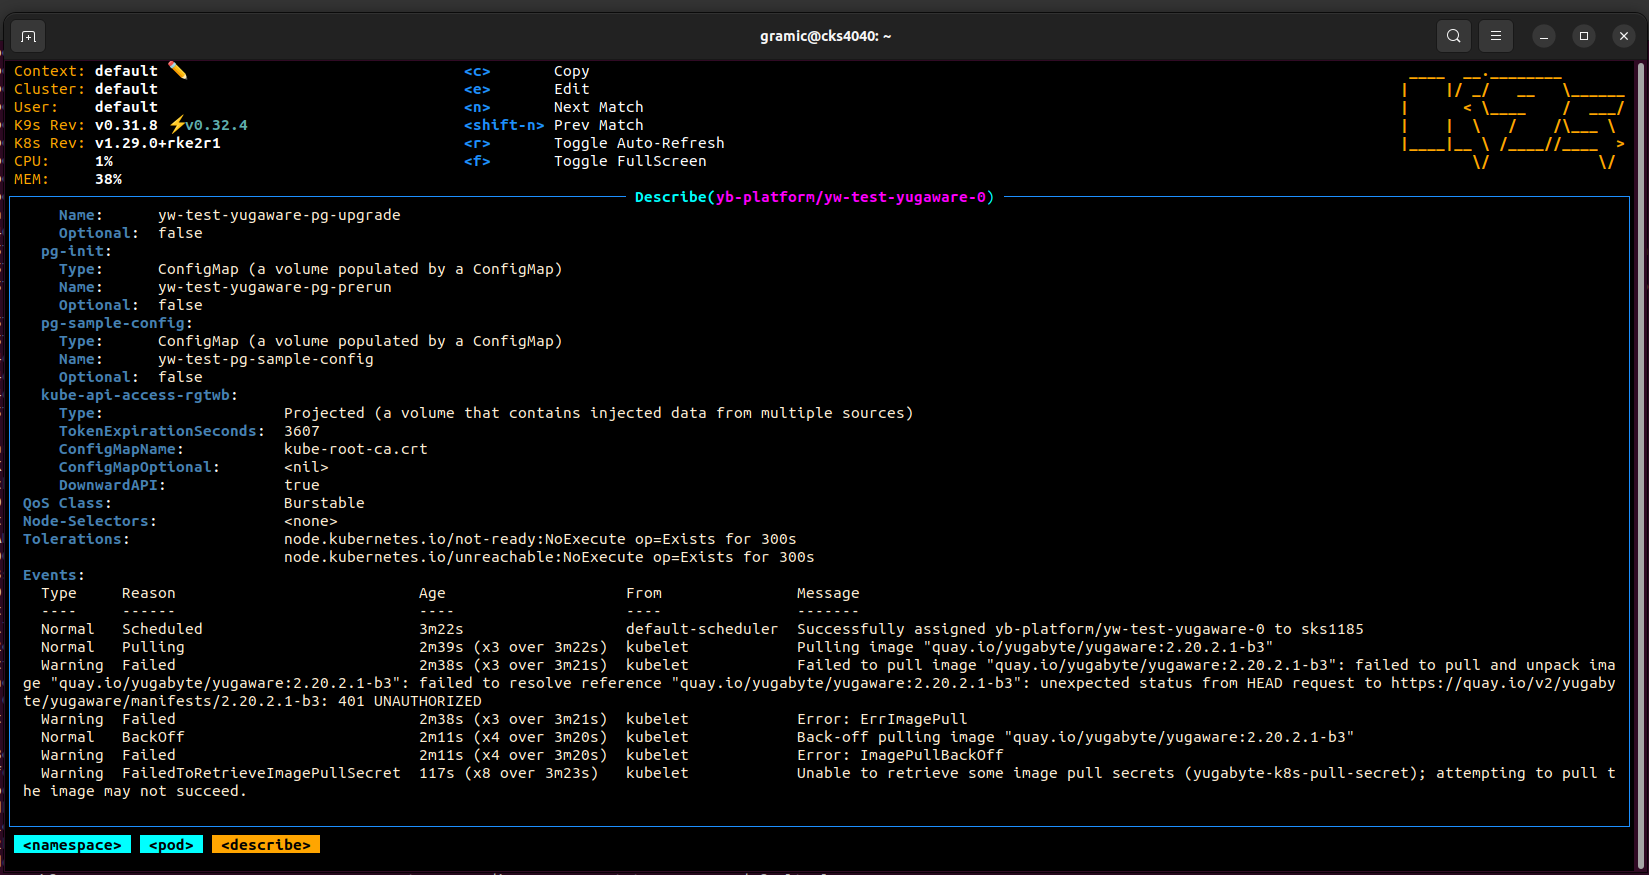
\includegraphics[width=1\linewidth]{source/implementation/evaluation/platforms/yugabytedb_pod_installation_subscription_interrup}
        \caption{yugabyteDB - Susbsription yugawre}
        \label{fig:yugabytedb_pod_installation_subscription_interrup}
    \end{figure}
\end{flushleft}
\begin{flushleft}
    Es stellte sich auch heraus, dass wenn man YugabyteDB 4 Cores pro Node zur Verfügung geben will (je zwei für den \texttt{master} und \texttt{tserver}),\\
    der Server mehr als 4 Cores haben muss.\\
    Andernfalls wird Kubernetes einen der beiden Pods nicht deployen, weil zuwenig Cores zur verfügung stehen.
\end{flushleft}
\begin{flushleft}
    Bei der konstelation \gls{rke2}, \Gls{Cilium} und \Gls{MetalLB}, muss nebst dem \texttt{IPAddressPool} auch ein \texttt{L2Advertisement} für den Pool gesetzt werden.\\
    Ansonsten kann die im YugabyteDB values.yaml gesetzte IP für den \texttt{tserver} von aussen nicht angesprochen werden:
    \lstset{style=gra_codestyle}
    \begin{lstlisting}[language=yaml, caption=metallb - Konfig YAML - Detail L2Advertisement,captionpos=b,label={lst:metallb-l2advertisement-setting},breaklines=true]
---
apiVersion: metallb.io/v1beta1
kind: L2Advertisement
metadata:
  name: l2adv
  namespace: metallb-system
spec:
  ipAddressPools:
  - distributed-sql
    \end{lstlisting}
    Dieses Problem ist schwer zu greifen und hat zwei Tage in Anspruch genommen, es zu Lösen.
    Die Vorschläge zum Lösen des Problems reichten von deakivieren von \texttt{kube-proxy} bis hin zu einer Migration zum \Gls{Cilium}-Loadb-Balancers.\\
    Mit diesem funktionierte dann nicht einmal mehr die Installation von yugabyteDB.\\
    Lösung brachte nur ein \texttt{GitHub}-Eintrag\cite{D4IZIEFN}, wo oben genannter Ansatz empfohlen wurde.
\end{flushleft}
\begin{flushleft}
    \paragraph{Konfiguration}
    Damit nicht der YugabyteDB Anywhere-Service installiert wird, muss das entsprechende Image gesetzt werden:
    \lstset{style=gra_codestyle}
    \begin{lstlisting}[language=yaml, caption=yugabyteDB - Helm Chart Manifest - Detail Image,captionpos=b,label={lst:yugabytedb-image-setting},breaklines=true]
...
Image:
  repository: "yugabytedb/yugabyte"
  tag: 2.20.2.1-b3
  pullPolicy: IfNotPresent
  pullSecretName: ""
...
    \end{lstlisting}

    Die StorageClass muss im \texttt{values.yaml} gesetzt werden, einmal für den \texttt{master} und einmal für den \texttt{tserver}
    \lstset{style=gra_codestyle}
    \begin{lstlisting}[language=yaml, caption=yugabyteDB - Helm Chart Manifest - Detail StorageClass,captionpos=b,label={lst:yugabytedb-storageclass-setting},breaklines=true]
...
storage:
  ephemeral: false  # will not allocate PVs when true
  master:
    count: 1
    size: 3Gi
    storageClass: "yb-storage"
  tserver:
    count: 1
    size: 3Gi
    storageClass: "yb-storage"
...
    \end{lstlisting}

    Dem node werden je 4 Cores zur verfügung gestellt.
    Zei für den \texttt{master} und zwei für den \texttt{tserver}.
    Beide erhalten 4GiB Memory:
    \lstset{style=gra_codestyle}
    \begin{lstlisting}[language=yaml, caption=yugabyteDB - Helm Chart Manifest - Detail Resources,captionpos=b,label={lst:yugabytedb-resources-setting},breaklines=true]
...
resource:
  master:
    requests:
      cpu: "1"
      memory: 2Gi
    limits:
      cpu: "1"
      ## Ensure the 'memory' value is strictly in 'Gi' or 'G' format. Deviating from these formats
      ## may result in setting an incorrect value for the 'memory_limit_hard_bytes' flag.
      ## Avoid using floating numbers for the numeric part of 'memory'. Doing so may lead to
      ## the 'memory_limit_hard_bytes' being set to 0, as the function expects integer values.
      memory: 2Gi
  tserver:
    requests:
      cpu: "1"
      memory: 4Gi
    limits:
      cpu: "1"
      ## Ensure the 'memory' value is strictly in 'Gi' or 'G' format. Deviating from these formats
      ## may result in setting an incorrect value for the 'memory_limit_hard_bytes' flag.
      ## Avoid using floating numbers for the numeric part of 'memory'. Doing so may lead to
      ## the 'memory_limit_hard_bytes' being set to 0, as the function expects integer values.
      memory: 4Gi
...
    \end{lstlisting}

    Die Shards, oder Tablets wie sie Yugabyte nennt, sollen auf allen drei Nodes repliziert werden:
    \lstset{style=gra_codestyle}
    \begin{lstlisting}[language=yaml, caption=yugabyteDB - Helm Chart Manifest - Detail Replika,captionpos=b,label={lst:yugabytedb-replica-setting},breaklines=true]
...
replicas:
  master: 3
  tserver: 3
  ## Used to set replication factor when isMultiAz is set to true
  totalMasters: 3
...
    \end{lstlisting}

    Wichtig ist auch, dass der \texttt{YSQL}-Dienst aktiv ist, damit PostgreSQL Abfragen abgesetzt werden können.\\
    Deshalb muss der Dienst aktiv sein und darf nicht deaktiviert werden:
    \lstset{style=gra_codestyle}
    \begin{lstlisting}[language=yaml, caption=yugabyteDB - Helm Chart Manifest - Detail Disable YSQL,captionpos=b,label={lst:yugabytedb-disableYsql-setting},breaklines=true]
...
# Disable the YSQL
disableYsql: false
...
    \end{lstlisting}

    Nun muss die Domain und die Service-Endpoints konfiguriert werden.\\
    Der Domainname bleibt vorerst \texttt{cluster.local} wie Default hinterlegt.\\
    Die Servicenamen und Ports werden nicht angetastet, wichtig ist die LoadBalancer-IP.\\
    Sie ist entsprechend der gewählten VirtualIP mit \texttt{10.0.20.106} zu setzen.

    \lstset{style=gra_codestyle}
    \begin{lstlisting}[language=yaml, caption=yugabyteDB - Helm Chart Manifest - Detail Domainname und Service-Endpoints,captionpos=b,label={lst:yugabytedb-domainname-serviceendpoints-setting},breaklines=true]
...
domainName: "cluster.local"

serviceEndpoints:
  - name: "yb-master-ui"
    type: LoadBalancer
    annotations: {}
    clusterIP: ""
    ## Sets the Service's externalTrafficPolicy
    externalTrafficPolicy: ""
    app: "yb-master"
    loadBalancerIP: ""
    ports:
      http-ui: "7000"

  - name: "yb-tserver-service"
    type: LoadBalancer
    annotations:
      metallb.universe.tf/loadBalancerIPs: 10.0.20.106
    clusterIP: ""
    ## Sets the Service's externalTrafficPolicy
    externalTrafficPolicy: ""
    app: "yb-tserver"
    loadBalancerIP: ""
    ports:
      tcp-yql-port: "9042"
      tcp-yedis-port: "6379"
      tcp-ysql-port: "5433"
...
    \end{lstlisting}
\end{flushleft}
\begin{flushleft}
    Beim Testen mit der höchsten Anzahl an Datensätzen zeigte sich, dass der \gls{local-path-provisioner} nicht sauber konfiguriert waren.\\
    Damit auf jedem Node die Persistence Volume Claims ausgeführt werden, müssen sie deklariert werden und in den StorageClass-Manifesten auch hinterlegt werden.\\
    Genauer muss in der \texttt{nodePathMap} folgende konfiguration vorgenommen werden:
\lstset{style=gra_codestyle}
\begin{lstlisting}[language=yaml, caption=local-path-provisioner nodePathMap,captionpos=b,label={lst:local-path-provisioner_nodePathMap},breaklines=true]
...
                "nodePathMap":[
                {
                        "node":"DEFAULT_PATH_FOR_NON_LISTED_NODES",
                        "paths":["<Lokaler Pfad>"]
                },
                {
                        "node":"<Nodename>",
                        "paths":["<Lokaler Pfad>"]
                },
...
\end{lstlisting}
    Hier ein Beispiel wie es mit den grossen Volumes aussieht:
\lstset{style=gra_codestyle}
\begin{lstlisting}[language=yaml, caption=local-path-provisioner nodePathMap Beispiel,captionpos=b,label={lst:local-path-provisioner_nodePathMap-exampl},breaklines=true]
...
                "nodePathMap":[
                {
                        "node":"DEFAULT_PATH_FOR_NON_LISTED_NODES",
                        "paths":["/srv/data/local-path-provisioner"]
                },
                {
                        "node":"sks1183",
                        "paths":["/srv/data/local-path-provisioner"]
                },
                {
                        "node":"sks1184",
                        "paths":["/srv/data/local-path-provisioner"]
                },
                {
                        "node":"sks1185",
                        "paths":["/srv/data/local-path-provisioner"]
                }
                ]
...
\end{lstlisting}
    Wird dies nicht gemacht, so wird auf den Default-Path geschrieben.\\
    Das ist zufällig und hat dann zur Folge, dass alle Volumes auf einem Node präsentiert werden.\\
    Was sehr schnell logischerweise dazu führt, dass zuwenig Diskspace vorhanden ist.\\
    Bei YugabyteDB kommt noch dazu, dass es zu Konflikten beim Schreiben von Blocks kommt.
\end{flushleft}
\begin{flushleft}
    Damit die Persistence Volumes sauber präsentiert werden, muss in der StorageClass die \texttt{nodeAffinity} gesetzt werden.\\
    Hier als Beispiel mit den Nodes \texttt{sks1183}, \texttt{sks1184} und \texttt{sks1185}:
\lstset{style=gra_codestyle}
\begin{lstlisting}[language=yaml, caption=yugabyteDB - StorageClass nodeAffinity,captionpos=b,label={lst:yugabytedb-storageclass_example},breaklines=true]
  nodeAffinity:
    required:
      nodeSelectorTerms:
      - matchExpressions:
        - key: kubernetes.io/hostname
          operator: In
          values:
          - sks1183
          - sks1184
          - sks1185
\end{lstlisting}
    \begin{warning}
        \textbf{hostPath}\\
        Der \texttt{hostPath} bei der StorageClass muss der gleiche sein, wie der Pfad im Node des nodePathMap von \gls{local-path-provisioner}.
        Auch sollten die Pfade auf allen Nodes gleich sein.
    \end{warning}
\end{flushleft}
\begin{flushleft}
    Die Problematik mit dem \texttt{nodePathMap} und der \texttt{nodeAffinity} auf der StorageClass hat auch rund zwei Arbeitstage in Anspruch genommen.
\end{flushleft}
    %! Author = gramic
%! Date = 03.04.24

% Preamble
\begin{flushleft}
    \subsection{sks9016 - yugabyteDB}
    \subsubsection{yugabyteDB - Download und Installation yugabyteDB}
    Ohne yugabyteDB zu installieren, lässt sich \texttt{ysql\_bench} nicht ausführen.
    Daher muss das ganze Package erst heruntergeladen werden:
    \lstset{style=gra_codestyle}
    \begin{lstlisting}[language=bash, caption=sks9016 - Download yugabyteDB On-Premise,captionpos=b,label={lst:sks9016-yugabytedb-download-on-premise},breaklines=true]
root@sks9016:~# wget https://downloads.yugabyte.com/releases/2.21.0.0/yugabyte-2.21.0.0-b545-linux-x86_64.tar.gz
    \end{lstlisting}
\end{flushleft}
\begin{flushleft}
    Im nächsten Schritt wird es im \texttt{/opt} entpackt und das \texttt{post\_install.sh}-Skript ausgeführt:
    \lstset{style=gra_codestyle}
    \begin{lstlisting}[language=bash, caption=sks9016 - Installation yugabyteDB On-Premise,captionpos=b,label={lst:sks9016-yugabytedb-install-on-premise},breaklines=true]
root@sks9016:/opt# tar xvfz yugabyte-2.21.0.0-b545-linux-x86_64.tar.gz && cd yugabyte-2.21.0.0/
...
root@sks9016:/opt/yugabyte-2.21.0.0# ./bin/post_install.sh
    \end{lstlisting}
\end{flushleft}
\begin{flushleft}
    Um nun zu Testen, ob das ganze Funktioniert, kann eine Verbindung zum Evaluationssystem hergestellt werden:
    \lstset{style=gra_codestyle}
    \begin{lstlisting}[language=bash, caption=sks9016 - Check yugabyteDB On-Premise,captionpos=b,label={lst:sks9016-yugabytedb-check-on-premise},breaklines=true]
root@sks9016:/opt/yugabyte-2.21.0.0# cd /opt/yugabyte-2.21.0.0/postgres/bin/
root@sks9016:/opt/yugabyte-2.21.0.0/postgres/bin# ./ysqlsh "host=10.0.20.106 user=yadmin"
Password for user yadmin:
ysqlsh (11.2-YB-2.21.0.0-b0)
Type "help" for help.

No entry for terminal type "xterm-256color";
using dumb terminal settings.
yugabyte=# exit
    \end{lstlisting}
    Damit ist der Benchmarking-Server ready.
\end{flushleft}
    %! Author = itgramic
%! Date = 05.12.23

% Preamble
\clearpage
\begin{flushleft}
    \subsubsection{Patroni}
    Patroni ist eine von Zalando auf Basis von Python entwickelte HA-Lösung für \Gls{PostgreSQL}.\\
    Patroni wird aktiv von Zalando gepflegt.
\end{flushleft}
\begin{flushleft}
    \paragraph{Core-Features}
    Patroni bietet folgende Core-Features:
    \begin{itemize}
        \item Rest-API und eigenes Skript- und Toolset
        \item Aktionen und Konfigurationen im Konsensprinzip abgestimmt
        \item Manueller oder Sheduled Switchover
        \item Reines PostgreSQL als Basis, Patroni setzt Hilfe von Python darauf auf
        \item Automatische reintegration von Nodes nach einem Fehler
        \item Citus kompatibel
        \item Docker und Docker-compose Dokumentation
    \end{itemize}
\end{flushleft}
\begin{flushleft}
    \paragraph{Replikation}
    Patroni bietet per Default eine eigene Replikation an.\\
    Diese ist allerdings eine asynchrone Replikation.
\begin{flushleft}
    Patroni unterstützt aber die synchrone Replikation von \Gls{PostgreSQL}.
\end{flushleft}
\end{flushleft}
\begin{flushleft}
    \paragraph{Proxy}
    Patroni benötigt einen \Gls{HAProxy}, um Load Balancing betreiben zu können\cite{VYXTI7BS}.
\end{flushleft}
\begin{flushleft}
    \paragraph{Pooling}
    Patroni benötigt einen externen \Gls{Connection Pooler}.\\
    Hier wird oft PgBouncer \cite{ATBELZ2X} verwendet.
\end{flushleft}
\begin{flushleft}
    \paragraph{API / Skripte}
    Patroni hat ein eigenes Tool- und Commandset, \texttt{patronictl}, welches die Verwaltung vereinfacht.\\
    Es umfasst das Ändern und Erfassen von Konfigurationen, das Forcieren eines Failovers als Switchover, Maintenance Handling und Informationsbeschaffung.\\
    Zusätzlich bietet Patroni eine API, welche Daten für das Monitoring bereitstellt,\\
    aber auch Betriebsfunktionen zur Verfügung stellt.\\
\end{flushleft}
\begin{flushleft}
    \paragraph{\gls{etcd}}
    Patroni benötigt etcd oder \Gls{Consul} als \Gls{Key-Value-Store}.
\end{flushleft}
\begin{flushleft}
    \paragraph{Architektur}
    Das Architektur-Schaubild sieht folgendermassen aus:
    \begin{figure}[H]
        \centering
        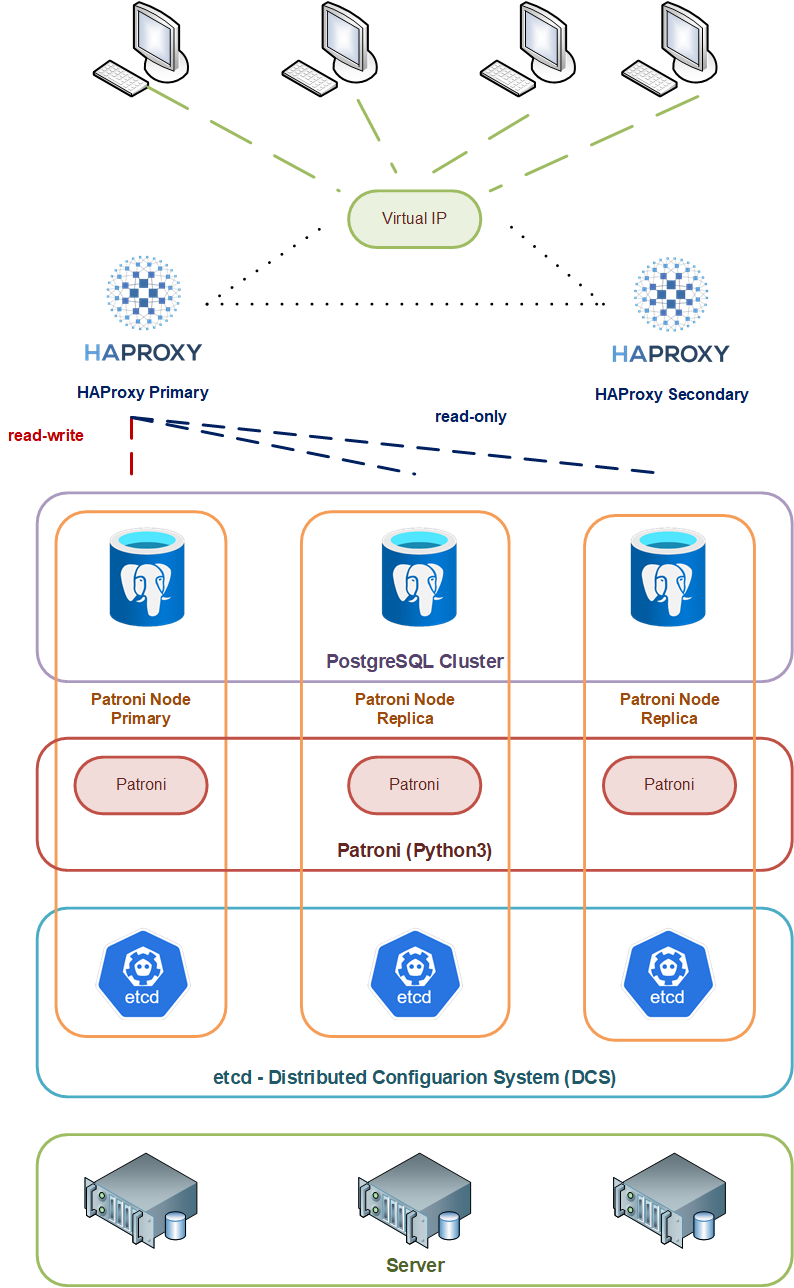
\includegraphics[width=0.7\linewidth]{source/implementation/evaluation/postgresql_ha_solutions/patroni_architecture}
        \caption{Patroni-Architektur}
        \label{fig:patroni-architecture}
    \end{figure}
\end{flushleft}
\begin{flushleft}
    \paragraph{Maintenance}
    Patroni ist ein sehr gepflegtes Projekt, welches die gängigen Community Standards einhält.\\
    Die Details sind im \hyperref[subsec:maintenance_patroni]{Anhang - Maintenance} zu finden.
\end{flushleft}
\begin{flushleft}
    \paragraph{Synergien und Mehrwert}
    Patroni kann nicht nur mit Citus zu einem Distributed / Sharded SQL System umgebaut werden,\\
    es ist auch Kern von StackGres.
\end{flushleft}
\begin{flushleft}
    Damit könnten die API und Skripte in beiden Welten verwendet werden.\\
    Der Aufwand für die Verwaltung und Optimierung würde stark gesenkt.\\
    Projekte wie \texttt{vitabaks / postgresql\_cluster}\cite{HIQVBEPF} bieten zudem die Vorlage für eine noch stärkere Automatisierung.
\end{flushleft}
    \subsubsection{Stackgres mit Citus}
\begin{flushleft} 
Stackgres ist eine PostgreSQL Implementation die dafür vorgesehenen ist, in einem Kubernetes Cluster betrieben zu werden.
\end{flushleft} 
\begin{flushleft}
An sich wäre Stackgres nur eine Implementation von Patroni in Kubernetes inkl. Load Balancer.\\
Nun kommt das Citus-Plugin ins spiel, welches aus einer jeden Monolithischen, Klassischen PostgreSQL Installation eine Distributed SQL Umgebung macht.////
Citus wiederum ist in den Microsoft Konzern eingebettet
\end{flushleft}

\begin{flushleft}
    \paragraph{Architektur}
    \begin{flushleft}
        \subparagraph{Citus Coordinator und Workers}
        \begin{figure}[H]
            \centering
            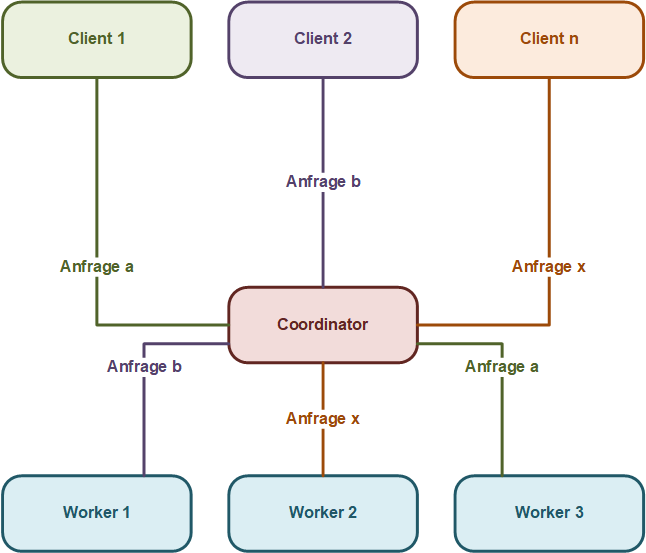
\includegraphics[width=0.75\linewidth]{source/implementation/evaluation/postgresql_ha_solutions/stackgres/citus_coordinator_worker}
            \caption{Citus - Coordinator und Workers}
            \label{fig:citus_coordinator_worker}
        \end{figure}
    \end{flushleft}
    \begin{flushleft}
        \subparagraph{Citus Sharding}
        Citus bietet zwei Sharding-Modelle an.
        \begin{flushleft}
            \textbf{Row-based sharding}
            Beim diesen sharding werden Tabellen anhand einer Distribution Column aufgeteilt. \cite{2Y5FA36C, FDUUL9IM}
        \end{flushleft}
        \begin{flushleft}
            \textbf{Schema-based sharding}
        \end{flushleft}
    \end{flushleft}
\end{flushleft}
\begin{flushleft}
    \paragraph{Maintenance}
    Bei Stackgres gab es im letzten Monat keine wirkliche Bewegung:
    \begin{figure}[H]
        \centering
        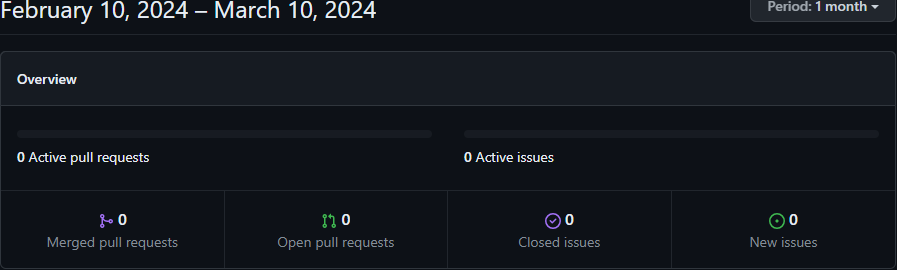
\includegraphics[width=0.75\linewidth]{source/implementation/evaluation/postgresql_ha_solutions/insights/stackgres_citus/pulse_ongres_stackgres}
        \caption{Stackgres - Pulse}
        \label{fig:pulse_ongres_stackgres}
    \end{figure}
    Anders sieht es bei Citus aus, die Firma die mittlerweile zu Microsoft gehört, schliesst Issues rasch und hat eine verhältnissmässig hohe Requstrate:
    \begin{figure}[H]
        \centering
        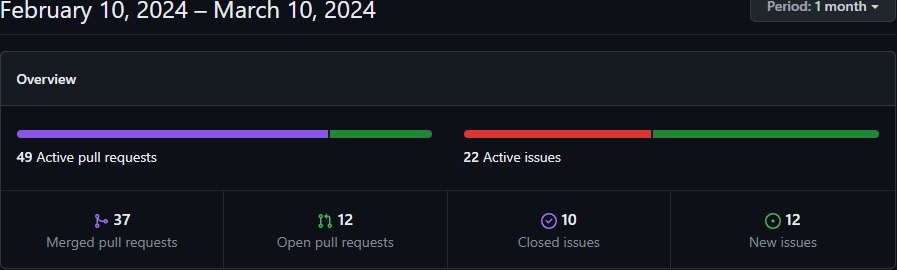
\includegraphics[width=0.75\linewidth]{source/implementation/evaluation/postgresql_ha_solutions/insights/stackgres_citus/pulse_citusdata_citus}
        \caption{Citus - Pulse}
        \label{fig:pulse_citusdata_citus}
    \end{figure}

    Bei Stackgres wird sehr viel Code hinzugefügt oder gelöscht, beim älteren Citus wurden weniger änderungen verzeichnet:
    \begin{figure}[H]
        \centering
        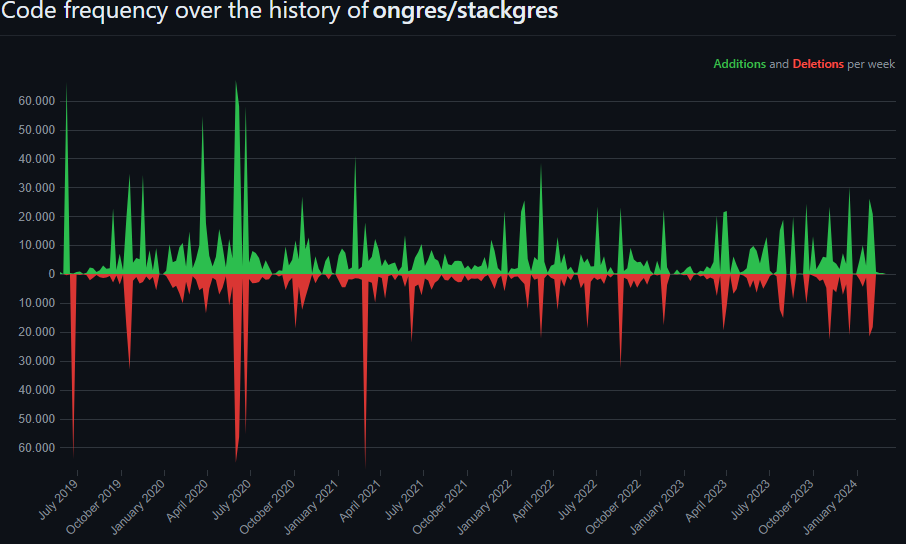
\includegraphics[width=0.75\linewidth]{source/implementation/evaluation/postgresql_ha_solutions/insights/stackgres_citus/code_frequency_ongres_stackgres}
        \caption{Stackgres - Code Frequency}
        \label{fig:code_frequency_ongres_stackgres}
    \end{figure}
    \begin{figure}[H]
        \centering
        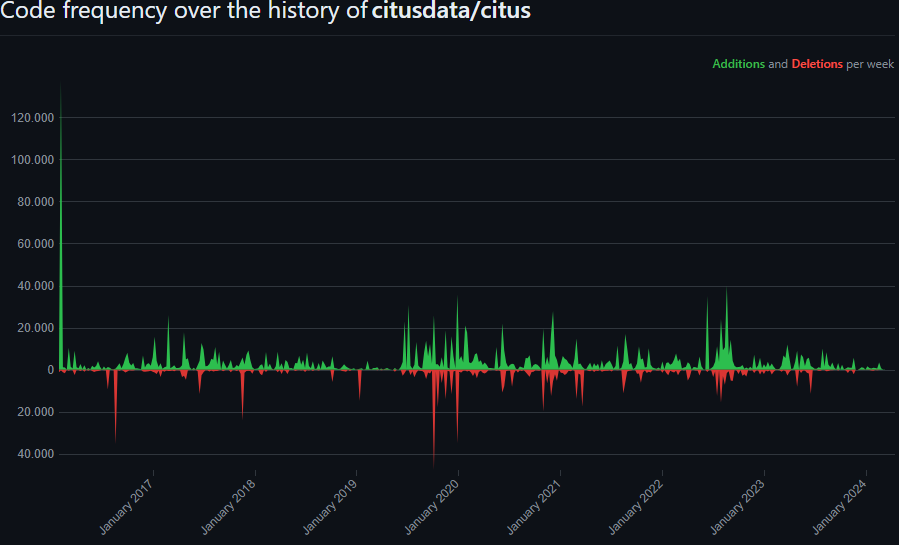
\includegraphics[width=0.75\linewidth]{source/implementation/evaluation/postgresql_ha_solutions/insights/stackgres_citus/code_frequency_citusdata_citus}
        \caption{Citus - Code Frequency}
        \label{fig:code_frequency_citusdata_citus}
    \end{figure}

    Citus legt einen hohen Stellenwert auf die Community-Standars, Stackgres selbst schneidet hier nur Mittelmässig ab:
    \begin{figure}[H]
        \centering
        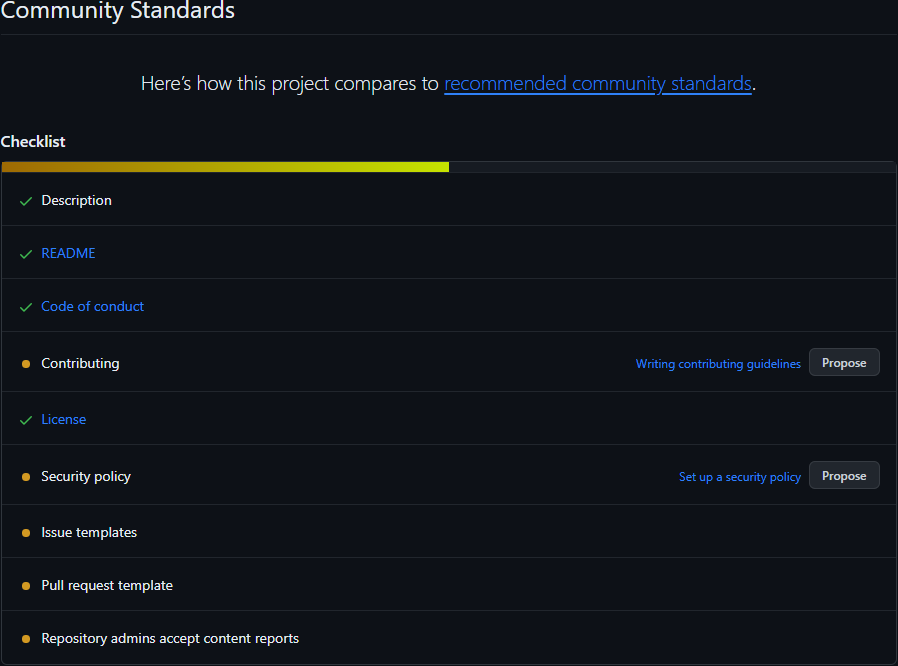
\includegraphics[width=0.75\linewidth]{source/implementation/evaluation/postgresql_ha_solutions/insights/stackgres_citus/stackgres_community_standards}
        \caption{Stackgres - Community Standards}
        \label{fig:stackgres_community_standards}
    \end{figure}
    \begin{figure}[H]
        \centering
        \includegraphics[width=0.75\linewidth]{source/implementation/evaluation/postgresql_ha_solutions/insights/stackgres_citus/citus_community_standards}
        \caption{Citus - Community Standards}
        \label{fig:citus_community_standards}
    \end{figure}

    Die Stackgres Constributors pflegen aktiv Additions ein, löschen Regelmässig und Commiten ebenfalls auf die main-Branch.
    Citus, dessen Repository länger Commited wird, hat weniger bewegung auf die main-Branch.
    \begin{figure}[H]
        \centering
        \includegraphics[width=0.75\linewidth]{source/implementation/evaluation/postgresql_ha_solutions/insights/stackgres_citus/contributors_commits_ongres_stackgres}
        \caption{Stackgres - Contributors Commits}
        \label{fig:contributors_commits_ongres_stackgres}
    \end{figure}
    \begin{figure}[H]
        \centering
        \includegraphics[width=0.75\linewidth]{source/implementation/evaluation/postgresql_ha_solutions/insights/stackgres_citus/contributors_deletations_ongres_stackgres}
        \caption{Stackgres - Contributors Deletations}
        \label{fig:contributors_deletations_ongres_stackgres}
    \end{figure}
    \begin{figure}[H]
        \centering
        \includegraphics[width=0.75\linewidth]{source/implementation/evaluation/postgresql_ha_solutions/insights/stackgres_citus/contributors_addition_ongres_stackgres}
        \caption{Stackgres - Contributors Additions}
        \label{fig:contributors_addition_ongres_stackgres}
    \end{figure}
    \begin{figure}[H]
        \centering
        \includegraphics[width=0.75\linewidth]{source/implementation/evaluation/postgresql_ha_solutions/insights/stackgres_citus/contributors_commits_citusdata_citus}
        \caption{Citus - Contributors Commits}
        \label{fig:contributors_commits_citusdata_citus}
    \end{figure}
    \begin{figure}[H]
        \centering
        \includegraphics[width=0.75\linewidth]{source/implementation/evaluation/postgresql_ha_solutions/insights/stackgres_citus/contributors_deletations_citusdata_citus}
        \caption{Citus - Contributors Deletations}
        \label{fig:contributors_deletations_citusdata_citus}
    \end{figure}
    \begin{figure}[H]
        \centering
        \includegraphics[width=0.75\linewidth]{source/implementation/evaluation/postgresql_ha_solutions/insights/stackgres_citus/contributors_additions_citusdata_citus}
        \caption{Citus - Contributors Additions}
        \label{fig:contributors_additions_citusdata_citus}
    \end{figure}

    Gerade Ende Januar gab es bei Stackgres eine grössere Anzahl Commits, anhand der statistik wird ersichtlich, dass i.d.R. einmal pro Monat grössere Mengen an Commits eingespielt werden.
    Bei Citus gibt es ebenfalls Regelmässig grössere Mengen an Commits, allerdings scheint bei citusdata mehr mit kürzeren Sprints gearbeitet zu werden als bei ongres denn die Commits sind Regelmässiger:
    \begin{figure}[H]
        \centering
        \includegraphics[width=0.75\linewidth]{source/implementation/evaluation/postgresql_ha_solutions/insights/stackgres_citus/commit_activity_ongres_stackgres}
        \caption{Stackgres - Commit Activity}
        \label{fig:commit_activity_ongres_stackgres}
    \end{figure}
    \begin{figure}[H]
        \centering
        \includegraphics[width=0.75\linewidth]{source/implementation/evaluation/postgresql_ha_solutions/insights/stackgres_citus/commit_activity_citusdata_citus}
        \caption{Citus - Commit Activity}
        \label{fig:commit_activity_citusdata_citus}
    \end{figure}

    In letzter Zeit haben nur ongres, der Entwickler von Stackgres, als auch citusdata, grössere Commits auf das Repository gefahren.
    Andere grössere Entwickler wie EnterpriseDB sind abwesend.
    \begin{figure}[H]
        \centering
        \includegraphics[width=0.75\linewidth]{source/implementation/evaluation/postgresql_ha_solutions/insights/stackgres_citus/network_graph_ongres_stackgres}
        \caption{Stackgres - Network Graph}
        \label{fig:network_graph_ongres_stackgres}
    \end{figure}
    \begin{figure}[H]
        \centering
        \includegraphics[width=0.75\linewidth]{source/implementation/evaluation/postgresql_ha_solutions/insights/stackgres_citus/network_graph_citusdata_citus}
        \caption{Citus - Network Graph}
        \label{fig:network_graph_citusdata_citus}
    \end{figure}

\end{flushleft}
\end{flushleft}
    %! Author = gramic
%! Date = 24.04.24

% Preamble
\begin{flushleft}
    \section{Evaluationssysteme - Benchmarking}
    %! Author = gramic
%! Date = 15.03.24

% Preamble
\begin{flushleft}
    \subsubsection{yugabyteDB}
    \paragraph{Installation}
    Wähend der Installation des YugabyteDB Evaluations-Enviroment wurde festgestellt, das man zwei Varianten Installieren kann.
    YugabyteDB (Repository yugabyte) und YugabyteDB Anywhere (Repository yugawre):
    \begin{figure}[H]
        \centering
        \includegraphics[width=1\linewidth]{source/implementation/evaluation/platforms/yugabytedb_pod_installation_subscription_interrup}
        \caption{yugabyteDB - Susbsription yugawre}
        \label{fig:yugabytedb_pod_installation_subscription_interrup}
    \end{figure}
\end{flushleft}
\begin{flushleft}
    Es stellte sich auch heraus, dass wenn man YugabyteDB 4 Cores pro Node zur Verfügung geben will (je zwei für den \texttt{master} und \texttt{tserver}),\\
    der Server mehr als 4 Cores haben muss.\\
    Andernfalls wird Kubernetes einen der beiden Pods nicht deployen, weil zuwenig Cores zur verfügung stehen.
\end{flushleft}
\begin{flushleft}
    Bei der konstelation \gls{rke2}, \Gls{Cilium} und \Gls{MetalLB}, muss nebst dem \texttt{IPAddressPool} auch ein \texttt{L2Advertisement} für den Pool gesetzt werden.\\
    Ansonsten kann die im YugabyteDB values.yaml gesetzte IP für den \texttt{tserver} von aussen nicht angesprochen werden:
    \lstset{style=gra_codestyle}
    \begin{lstlisting}[language=yaml, caption=metallb - Konfig YAML - Detail L2Advertisement,captionpos=b,label={lst:metallb-l2advertisement-setting},breaklines=true]
---
apiVersion: metallb.io/v1beta1
kind: L2Advertisement
metadata:
  name: l2adv
  namespace: metallb-system
spec:
  ipAddressPools:
  - distributed-sql
    \end{lstlisting}
    Dieses Problem ist schwer zu greifen und hat zwei Tage in Anspruch genommen, es zu Lösen.
    Die Vorschläge zum Lösen des Problems reichten von deakivieren von \texttt{kube-proxy} bis hin zu einer Migration zum \Gls{Cilium}-Loadb-Balancers.\\
    Mit diesem funktionierte dann nicht einmal mehr die Installation von yugabyteDB.\\
    Lösung brachte nur ein \texttt{GitHub}-Eintrag\cite{D4IZIEFN}, wo oben genannter Ansatz empfohlen wurde.
\end{flushleft}
\begin{flushleft}
    \paragraph{Konfiguration}
    Damit nicht der YugabyteDB Anywhere-Service installiert wird, muss das entsprechende Image gesetzt werden:
    \lstset{style=gra_codestyle}
    \begin{lstlisting}[language=yaml, caption=yugabyteDB - Helm Chart Manifest - Detail Image,captionpos=b,label={lst:yugabytedb-image-setting},breaklines=true]
...
Image:
  repository: "yugabytedb/yugabyte"
  tag: 2.20.2.1-b3
  pullPolicy: IfNotPresent
  pullSecretName: ""
...
    \end{lstlisting}

    Die StorageClass muss im \texttt{values.yaml} gesetzt werden, einmal für den \texttt{master} und einmal für den \texttt{tserver}
    \lstset{style=gra_codestyle}
    \begin{lstlisting}[language=yaml, caption=yugabyteDB - Helm Chart Manifest - Detail StorageClass,captionpos=b,label={lst:yugabytedb-storageclass-setting},breaklines=true]
...
storage:
  ephemeral: false  # will not allocate PVs when true
  master:
    count: 1
    size: 3Gi
    storageClass: "yb-storage"
  tserver:
    count: 1
    size: 3Gi
    storageClass: "yb-storage"
...
    \end{lstlisting}

    Dem node werden je 4 Cores zur verfügung gestellt.
    Zei für den \texttt{master} und zwei für den \texttt{tserver}.
    Beide erhalten 4GiB Memory:
    \lstset{style=gra_codestyle}
    \begin{lstlisting}[language=yaml, caption=yugabyteDB - Helm Chart Manifest - Detail Resources,captionpos=b,label={lst:yugabytedb-resources-setting},breaklines=true]
...
resource:
  master:
    requests:
      cpu: "1"
      memory: 2Gi
    limits:
      cpu: "1"
      ## Ensure the 'memory' value is strictly in 'Gi' or 'G' format. Deviating from these formats
      ## may result in setting an incorrect value for the 'memory_limit_hard_bytes' flag.
      ## Avoid using floating numbers for the numeric part of 'memory'. Doing so may lead to
      ## the 'memory_limit_hard_bytes' being set to 0, as the function expects integer values.
      memory: 2Gi
  tserver:
    requests:
      cpu: "1"
      memory: 4Gi
    limits:
      cpu: "1"
      ## Ensure the 'memory' value is strictly in 'Gi' or 'G' format. Deviating from these formats
      ## may result in setting an incorrect value for the 'memory_limit_hard_bytes' flag.
      ## Avoid using floating numbers for the numeric part of 'memory'. Doing so may lead to
      ## the 'memory_limit_hard_bytes' being set to 0, as the function expects integer values.
      memory: 4Gi
...
    \end{lstlisting}

    Die Shards, oder Tablets wie sie Yugabyte nennt, sollen auf allen drei Nodes repliziert werden:
    \lstset{style=gra_codestyle}
    \begin{lstlisting}[language=yaml, caption=yugabyteDB - Helm Chart Manifest - Detail Replika,captionpos=b,label={lst:yugabytedb-replica-setting},breaklines=true]
...
replicas:
  master: 3
  tserver: 3
  ## Used to set replication factor when isMultiAz is set to true
  totalMasters: 3
...
    \end{lstlisting}

    Wichtig ist auch, dass der \texttt{YSQL}-Dienst aktiv ist, damit PostgreSQL Abfragen abgesetzt werden können.\\
    Deshalb muss der Dienst aktiv sein und darf nicht deaktiviert werden:
    \lstset{style=gra_codestyle}
    \begin{lstlisting}[language=yaml, caption=yugabyteDB - Helm Chart Manifest - Detail Disable YSQL,captionpos=b,label={lst:yugabytedb-disableYsql-setting},breaklines=true]
...
# Disable the YSQL
disableYsql: false
...
    \end{lstlisting}

    Nun muss die Domain und die Service-Endpoints konfiguriert werden.\\
    Der Domainname bleibt vorerst \texttt{cluster.local} wie Default hinterlegt.\\
    Die Servicenamen und Ports werden nicht angetastet, wichtig ist die LoadBalancer-IP.\\
    Sie ist entsprechend der gewählten VirtualIP mit \texttt{10.0.20.106} zu setzen.

    \lstset{style=gra_codestyle}
    \begin{lstlisting}[language=yaml, caption=yugabyteDB - Helm Chart Manifest - Detail Domainname und Service-Endpoints,captionpos=b,label={lst:yugabytedb-domainname-serviceendpoints-setting},breaklines=true]
...
domainName: "cluster.local"

serviceEndpoints:
  - name: "yb-master-ui"
    type: LoadBalancer
    annotations: {}
    clusterIP: ""
    ## Sets the Service's externalTrafficPolicy
    externalTrafficPolicy: ""
    app: "yb-master"
    loadBalancerIP: ""
    ports:
      http-ui: "7000"

  - name: "yb-tserver-service"
    type: LoadBalancer
    annotations:
      metallb.universe.tf/loadBalancerIPs: 10.0.20.106
    clusterIP: ""
    ## Sets the Service's externalTrafficPolicy
    externalTrafficPolicy: ""
    app: "yb-tserver"
    loadBalancerIP: ""
    ports:
      tcp-yql-port: "9042"
      tcp-yedis-port: "6379"
      tcp-ysql-port: "5433"
...
    \end{lstlisting}
\end{flushleft}
\begin{flushleft}
    Beim Testen mit der höchsten Anzahl an Datensätzen zeigte sich, dass der \gls{local-path-provisioner} nicht sauber konfiguriert waren.\\
    Damit auf jedem Node die Persistence Volume Claims ausgeführt werden, müssen sie deklariert werden und in den StorageClass-Manifesten auch hinterlegt werden.\\
    Genauer muss in der \texttt{nodePathMap} folgende konfiguration vorgenommen werden:
\lstset{style=gra_codestyle}
\begin{lstlisting}[language=yaml, caption=local-path-provisioner nodePathMap,captionpos=b,label={lst:local-path-provisioner_nodePathMap},breaklines=true]
...
                "nodePathMap":[
                {
                        "node":"DEFAULT_PATH_FOR_NON_LISTED_NODES",
                        "paths":["<Lokaler Pfad>"]
                },
                {
                        "node":"<Nodename>",
                        "paths":["<Lokaler Pfad>"]
                },
...
\end{lstlisting}
    Hier ein Beispiel wie es mit den grossen Volumes aussieht:
\lstset{style=gra_codestyle}
\begin{lstlisting}[language=yaml, caption=local-path-provisioner nodePathMap Beispiel,captionpos=b,label={lst:local-path-provisioner_nodePathMap-exampl},breaklines=true]
...
                "nodePathMap":[
                {
                        "node":"DEFAULT_PATH_FOR_NON_LISTED_NODES",
                        "paths":["/srv/data/local-path-provisioner"]
                },
                {
                        "node":"sks1183",
                        "paths":["/srv/data/local-path-provisioner"]
                },
                {
                        "node":"sks1184",
                        "paths":["/srv/data/local-path-provisioner"]
                },
                {
                        "node":"sks1185",
                        "paths":["/srv/data/local-path-provisioner"]
                }
                ]
...
\end{lstlisting}
    Wird dies nicht gemacht, so wird auf den Default-Path geschrieben.\\
    Das ist zufällig und hat dann zur Folge, dass alle Volumes auf einem Node präsentiert werden.\\
    Was sehr schnell logischerweise dazu führt, dass zuwenig Diskspace vorhanden ist.\\
    Bei YugabyteDB kommt noch dazu, dass es zu Konflikten beim Schreiben von Blocks kommt.
\end{flushleft}
\begin{flushleft}
    Damit die Persistence Volumes sauber präsentiert werden, muss in der StorageClass die \texttt{nodeAffinity} gesetzt werden.\\
    Hier als Beispiel mit den Nodes \texttt{sks1183}, \texttt{sks1184} und \texttt{sks1185}:
\lstset{style=gra_codestyle}
\begin{lstlisting}[language=yaml, caption=yugabyteDB - StorageClass nodeAffinity,captionpos=b,label={lst:yugabytedb-storageclass_example},breaklines=true]
  nodeAffinity:
    required:
      nodeSelectorTerms:
      - matchExpressions:
        - key: kubernetes.io/hostname
          operator: In
          values:
          - sks1183
          - sks1184
          - sks1185
\end{lstlisting}
    \begin{warning}
        \textbf{hostPath}\\
        Der \texttt{hostPath} bei der StorageClass muss der gleiche sein, wie der Pfad im Node des nodePathMap von \gls{local-path-provisioner}.
        Auch sollten die Pfade auf allen Nodes gleich sein.
    \end{warning}
\end{flushleft}
\begin{flushleft}
    Die Problematik mit dem \texttt{nodePathMap} und der \texttt{nodeAffinity} auf der StorageClass hat auch rund zwei Arbeitstage in Anspruch genommen.
\end{flushleft}
    %! Author = itgramic
%! Date = 05.12.23

% Preamble
\clearpage
\begin{flushleft}
    \subsubsection{Patroni}
    Patroni ist eine von Zalando auf Basis von Python entwickelte HA-Lösung für \Gls{PostgreSQL}.\\
    Patroni wird aktiv von Zalando gepflegt.
\end{flushleft}
\begin{flushleft}
    \paragraph{Core-Features}
    Patroni bietet folgende Core-Features:
    \begin{itemize}
        \item Rest-API und eigenes Skript- und Toolset
        \item Aktionen und Konfigurationen im Konsensprinzip abgestimmt
        \item Manueller oder Sheduled Switchover
        \item Reines PostgreSQL als Basis, Patroni setzt Hilfe von Python darauf auf
        \item Automatische reintegration von Nodes nach einem Fehler
        \item Citus kompatibel
        \item Docker und Docker-compose Dokumentation
    \end{itemize}
\end{flushleft}
\begin{flushleft}
    \paragraph{Replikation}
    Patroni bietet per Default eine eigene Replikation an.\\
    Diese ist allerdings eine asynchrone Replikation.
\begin{flushleft}
    Patroni unterstützt aber die synchrone Replikation von \Gls{PostgreSQL}.
\end{flushleft}
\end{flushleft}
\begin{flushleft}
    \paragraph{Proxy}
    Patroni benötigt einen \Gls{HAProxy}, um Load Balancing betreiben zu können\cite{VYXTI7BS}.
\end{flushleft}
\begin{flushleft}
    \paragraph{Pooling}
    Patroni benötigt einen externen \Gls{Connection Pooler}.\\
    Hier wird oft PgBouncer \cite{ATBELZ2X} verwendet.
\end{flushleft}
\begin{flushleft}
    \paragraph{API / Skripte}
    Patroni hat ein eigenes Tool- und Commandset, \texttt{patronictl}, welches die Verwaltung vereinfacht.\\
    Es umfasst das Ändern und Erfassen von Konfigurationen, das Forcieren eines Failovers als Switchover, Maintenance Handling und Informationsbeschaffung.\\
    Zusätzlich bietet Patroni eine API, welche Daten für das Monitoring bereitstellt,\\
    aber auch Betriebsfunktionen zur Verfügung stellt.\\
\end{flushleft}
\begin{flushleft}
    \paragraph{\gls{etcd}}
    Patroni benötigt etcd oder \Gls{Consul} als \Gls{Key-Value-Store}.
\end{flushleft}
\begin{flushleft}
    \paragraph{Architektur}
    Das Architektur-Schaubild sieht folgendermassen aus:
    \begin{figure}[H]
        \centering
        \includegraphics[width=0.7\linewidth]{source/implementation/evaluation/postgresql_ha_solutions/patroni_architecture}
        \caption{Patroni-Architektur}
        \label{fig:patroni-architecture}
    \end{figure}
\end{flushleft}
\begin{flushleft}
    \paragraph{Maintenance}
    Patroni ist ein sehr gepflegtes Projekt, welches die gängigen Community Standards einhält.\\
    Die Details sind im \hyperref[subsec:maintenance_patroni]{Anhang - Maintenance} zu finden.
\end{flushleft}
\begin{flushleft}
    \paragraph{Synergien und Mehrwert}
    Patroni kann nicht nur mit Citus zu einem Distributed / Sharded SQL System umgebaut werden,\\
    es ist auch Kern von StackGres.
\end{flushleft}
\begin{flushleft}
    Damit könnten die API und Skripte in beiden Welten verwendet werden.\\
    Der Aufwand für die Verwaltung und Optimierung würde stark gesenkt.\\
    Projekte wie \texttt{vitabaks / postgresql\_cluster}\cite{HIQVBEPF} bieten zudem die Vorlage für eine noch stärkere Automatisierung.
\end{flushleft}
    \subsubsection{Stackgres mit Citus}
\begin{flushleft} 
Stackgres ist eine PostgreSQL Implementation die dafür vorgesehenen ist, in einem Kubernetes Cluster betrieben zu werden.
\end{flushleft} 
\begin{flushleft}
An sich wäre Stackgres nur eine Implementation von Patroni in Kubernetes inkl. Load Balancer.\\
Nun kommt das Citus-Plugin ins spiel, welches aus einer jeden Monolithischen, Klassischen PostgreSQL Installation eine Distributed SQL Umgebung macht.////
Citus wiederum ist in den Microsoft Konzern eingebettet
\end{flushleft}

\begin{flushleft}
    \paragraph{Architektur}
    \begin{flushleft}
        \subparagraph{Citus Coordinator und Workers}
        \begin{figure}[H]
            \centering
            \includegraphics[width=0.75\linewidth]{source/implementation/evaluation/postgresql_ha_solutions/stackgres/citus_coordinator_worker}
            \caption{Citus - Coordinator und Workers}
            \label{fig:citus_coordinator_worker}
        \end{figure}
    \end{flushleft}
    \begin{flushleft}
        \subparagraph{Citus Sharding}
        Citus bietet zwei Sharding-Modelle an.
        \begin{flushleft}
            \textbf{Row-based sharding}
            Beim diesen sharding werden Tabellen anhand einer Distribution Column aufgeteilt. \cite{2Y5FA36C, FDUUL9IM}
        \end{flushleft}
        \begin{flushleft}
            \textbf{Schema-based sharding}
        \end{flushleft}
    \end{flushleft}
\end{flushleft}
\begin{flushleft}
    \paragraph{Maintenance}
    Bei Stackgres gab es im letzten Monat keine wirkliche Bewegung:
    \begin{figure}[H]
        \centering
        \includegraphics[width=0.75\linewidth]{source/implementation/evaluation/postgresql_ha_solutions/insights/stackgres_citus/pulse_ongres_stackgres}
        \caption{Stackgres - Pulse}
        \label{fig:pulse_ongres_stackgres}
    \end{figure}
    Anders sieht es bei Citus aus, die Firma die mittlerweile zu Microsoft gehört, schliesst Issues rasch und hat eine verhältnissmässig hohe Requstrate:
    \begin{figure}[H]
        \centering
        \includegraphics[width=0.75\linewidth]{source/implementation/evaluation/postgresql_ha_solutions/insights/stackgres_citus/pulse_citusdata_citus}
        \caption{Citus - Pulse}
        \label{fig:pulse_citusdata_citus}
    \end{figure}

    Bei Stackgres wird sehr viel Code hinzugefügt oder gelöscht, beim älteren Citus wurden weniger änderungen verzeichnet:
    \begin{figure}[H]
        \centering
        \includegraphics[width=0.75\linewidth]{source/implementation/evaluation/postgresql_ha_solutions/insights/stackgres_citus/code_frequency_ongres_stackgres}
        \caption{Stackgres - Code Frequency}
        \label{fig:code_frequency_ongres_stackgres}
    \end{figure}
    \begin{figure}[H]
        \centering
        \includegraphics[width=0.75\linewidth]{source/implementation/evaluation/postgresql_ha_solutions/insights/stackgres_citus/code_frequency_citusdata_citus}
        \caption{Citus - Code Frequency}
        \label{fig:code_frequency_citusdata_citus}
    \end{figure}

    Citus legt einen hohen Stellenwert auf die Community-Standars, Stackgres selbst schneidet hier nur Mittelmässig ab:
    \begin{figure}[H]
        \centering
        \includegraphics[width=0.75\linewidth]{source/implementation/evaluation/postgresql_ha_solutions/insights/stackgres_citus/stackgres_community_standards}
        \caption{Stackgres - Community Standards}
        \label{fig:stackgres_community_standards}
    \end{figure}
    \begin{figure}[H]
        \centering
        \includegraphics[width=0.75\linewidth]{source/implementation/evaluation/postgresql_ha_solutions/insights/stackgres_citus/citus_community_standards}
        \caption{Citus - Community Standards}
        \label{fig:citus_community_standards}
    \end{figure}

    Die Stackgres Constributors pflegen aktiv Additions ein, löschen Regelmässig und Commiten ebenfalls auf die main-Branch.
    Citus, dessen Repository länger Commited wird, hat weniger bewegung auf die main-Branch.
    \begin{figure}[H]
        \centering
        \includegraphics[width=0.75\linewidth]{source/implementation/evaluation/postgresql_ha_solutions/insights/stackgres_citus/contributors_commits_ongres_stackgres}
        \caption{Stackgres - Contributors Commits}
        \label{fig:contributors_commits_ongres_stackgres}
    \end{figure}
    \begin{figure}[H]
        \centering
        \includegraphics[width=0.75\linewidth]{source/implementation/evaluation/postgresql_ha_solutions/insights/stackgres_citus/contributors_deletations_ongres_stackgres}
        \caption{Stackgres - Contributors Deletations}
        \label{fig:contributors_deletations_ongres_stackgres}
    \end{figure}
    \begin{figure}[H]
        \centering
        \includegraphics[width=0.75\linewidth]{source/implementation/evaluation/postgresql_ha_solutions/insights/stackgres_citus/contributors_addition_ongres_stackgres}
        \caption{Stackgres - Contributors Additions}
        \label{fig:contributors_addition_ongres_stackgres}
    \end{figure}
    \begin{figure}[H]
        \centering
        \includegraphics[width=0.75\linewidth]{source/implementation/evaluation/postgresql_ha_solutions/insights/stackgres_citus/contributors_commits_citusdata_citus}
        \caption{Citus - Contributors Commits}
        \label{fig:contributors_commits_citusdata_citus}
    \end{figure}
    \begin{figure}[H]
        \centering
        \includegraphics[width=0.75\linewidth]{source/implementation/evaluation/postgresql_ha_solutions/insights/stackgres_citus/contributors_deletations_citusdata_citus}
        \caption{Citus - Contributors Deletations}
        \label{fig:contributors_deletations_citusdata_citus}
    \end{figure}
    \begin{figure}[H]
        \centering
        \includegraphics[width=0.75\linewidth]{source/implementation/evaluation/postgresql_ha_solutions/insights/stackgres_citus/contributors_additions_citusdata_citus}
        \caption{Citus - Contributors Additions}
        \label{fig:contributors_additions_citusdata_citus}
    \end{figure}

    Gerade Ende Januar gab es bei Stackgres eine grössere Anzahl Commits, anhand der statistik wird ersichtlich, dass i.d.R. einmal pro Monat grössere Mengen an Commits eingespielt werden.
    Bei Citus gibt es ebenfalls Regelmässig grössere Mengen an Commits, allerdings scheint bei citusdata mehr mit kürzeren Sprints gearbeitet zu werden als bei ongres denn die Commits sind Regelmässiger:
    \begin{figure}[H]
        \centering
        \includegraphics[width=0.75\linewidth]{source/implementation/evaluation/postgresql_ha_solutions/insights/stackgres_citus/commit_activity_ongres_stackgres}
        \caption{Stackgres - Commit Activity}
        \label{fig:commit_activity_ongres_stackgres}
    \end{figure}
    \begin{figure}[H]
        \centering
        \includegraphics[width=0.75\linewidth]{source/implementation/evaluation/postgresql_ha_solutions/insights/stackgres_citus/commit_activity_citusdata_citus}
        \caption{Citus - Commit Activity}
        \label{fig:commit_activity_citusdata_citus}
    \end{figure}

    In letzter Zeit haben nur ongres, der Entwickler von Stackgres, als auch citusdata, grössere Commits auf das Repository gefahren.
    Andere grössere Entwickler wie EnterpriseDB sind abwesend.
    \begin{figure}[H]
        \centering
        \includegraphics[width=0.75\linewidth]{source/implementation/evaluation/postgresql_ha_solutions/insights/stackgres_citus/network_graph_ongres_stackgres}
        \caption{Stackgres - Network Graph}
        \label{fig:network_graph_ongres_stackgres}
    \end{figure}
    \begin{figure}[H]
        \centering
        \includegraphics[width=0.75\linewidth]{source/implementation/evaluation/postgresql_ha_solutions/insights/stackgres_citus/network_graph_citusdata_citus}
        \caption{Citus - Network Graph}
        \label{fig:network_graph_citusdata_citus}
    \end{figure}

\end{flushleft}
\end{flushleft}
    %! Author = gramic
%! Date = 08.04.24

% Preamble
\begin{flushleft}
    \subsection{Testing Evaluationssysteme}
    %%! Author = gramic
%! Date = 08.04.24

% Preamble
\begin{flushleft}
    \subsubsection{Evaluation - Testfälle}
    \paragraph{Patroni}
    \begin{description}
        \item \textbf{Failover}\hfill \\
        \begin{enumerate}
            \item Der Server des Primary-Node wird manuell heruntergefahren.
            \item Während dem Failover müssen Daten via SQL\\eingeführt und ausgelesen werden.
            \item Während dem Failover muss mindestens eine längere Abfrage gestartet werden.
        \end{enumerate}
        \item \textbf{Switchover}\hfill \\
%        \setcounter{enumi}{4}
        \begin{enumerate}[resume]
            \item Mit der REST-API wird der Switchover\\auf einen anderen Nod abgesetzt.
            \item Mit dem \texttt{patronictl}-Command wird der Switchover gesetzt
            \item Während dem Switchover müssen Daten via SQL\\eingeführt und ausgelesen werden.
            \item Während dem Switchover muss mindestens eine längere Abfrage gestartet werden.
        \end{enumerate}
        \item \textbf{Restore}\hfill \\
%        \setcounter{enumi}{9}
        \begin{enumerate}[resume]
            \item Mit der REST-API wird der Node erst mit dem \texttt{reinitialize} wiederhergestellt\\und dann mit einem Switchover wieder als Primary gesetzt.
            \item Mit dem \texttt{patronictl}-Commandund Parameter \texttt{reinit} der Node wiederhergestellt\\und abschliessend mittels Switchover wieder als Primary gesetzt.
            \item Mit der REST-API wird der Node mit dem \texttt{reinitialize} wiederhergestellt
            \item Mit dem \texttt{patronictl}-Commandund Parameter \texttt{reinit} der Node wiederhergestellt
            \item Vor, während und nach dem Restore müssen Tabellen mit Foreign-Key-Constraints und Daten geprüft werden.
            \item Während dem Restore muss mindestens eine längere Abfrage gestartet werden und Daten via SQL\\eingeführt und ausgelesen werden.
        \end{enumerate}
    \end{description}
    \paragraph{StackGres - Citus}
    \begin{description}
        \item \textbf{Failover}\hfill \\
        \begin{enumerate}
            \item Der Server des Leader-Cooordinator-Node wird manuell heruntergefahren.
            \item Während dem Failover müssen Daten via SQL\\eingeführt und ausgelesen werden.
            \item Während dem Failover muss mindestens eine längere Abfrage gestartet werden.
        \end{enumerate}
        \item \textbf{Sharding}\hfill \\
%        \setcounter{enumi}{4}
        \begin{enumerate}[resume]
            \item Vor, während und nach dem Failover müssen Tabellen mit Foreign-Key-Constraints geprüft werden.
            \item Nach einem Failover-Test müssen alle Daten vorhanden sein.
        \end{enumerate}
        \item \textbf{Self Healing}\hfill \\
        \begin{enumerate}[resume]
            \item Der Node muss wieder hochgefahren werden.\\Der Node muss selbstständig Daten synchronisieren.
            \item Der Leader muss automatisch neu gesetzt werden, wenn notwendig
        \end{enumerate}
    \end{description}
    \paragraph{YugabyteDB}
    \begin{description}
        \item \textbf{Failover}\hfill \\
        \begin{enumerate}
            \item Ein k8s Node wird manuell heruntergefahren,\\indem der entsprechende Server heruntergefahren wird.
            \item Während dem Failover müssen Daten via SQL\\eingeführt und ausgelesen werden.
            \item Während dem Failover muss mindestens eine längere Abfrage gestartet werden.
        \end{enumerate}
        \item \textbf{Sharding}\hfill \\
%        \setcounter{enumi}{4}
        \begin{enumerate}[resume]
            \item Vor, während und nach dem Failover müssen Tabellen mit Foreign-Key-Constraints geprüft werden.
            \item Nach einem Failover-Test müssen alle Daten vorhanden sein.
        \end{enumerate}
        \item \textbf{Self Healing}\hfill \\
        \begin{enumerate}[resume]
            \item Der Node muss wieder hochgefahren werden.\\Der Node muss selbstständig Daten synchronisieren.
        \end{enumerate}
    \end{description}
\end{flushleft}
\begin{flushleft}
    \subsubsection{Evaluation - ERD self\_healing\_test}
    \label{subsubsec:erd_self_healing_test}
    Die Tests müssen bei allen drei Varianten anhand der Datenbank \texttt{self\_healing\_test} durchgeführt werden.\\
    Dabei werden die Tabellen, im hinblick auf das Citus Schema Based Sharding, in Schemas organisiert.\\
    Zwischen den einzelnen Schemas sollen einige Tabellen einen Foreign-Key auf andere Tabellen legen:
    \begin{figure}[H]
        \centering
        \includegraphics[width=0.5\linewidth]{source/implementation/evaluation/evaluation_tests/erd_self_healing_test}
        \caption{Testing - ERD DB self\_healing\_test}
        \label{fig:erd_self_healing_test}
    \end{figure}
\end{flushleft}
    %%! Author = gramic
%! Date = 15.03.24

% Preamble
\begin{flushleft}
    \subsubsection{yugabyteDB}
    \paragraph{Installation}
    Wähend der Installation des YugabyteDB Evaluations-Enviroment wurde festgestellt, das man zwei Varianten Installieren kann.
    YugabyteDB (Repository yugabyte) und YugabyteDB Anywhere (Repository yugawre):
    \begin{figure}[H]
        \centering
        \includegraphics[width=1\linewidth]{source/implementation/evaluation/platforms/yugabytedb_pod_installation_subscription_interrup}
        \caption{yugabyteDB - Susbsription yugawre}
        \label{fig:yugabytedb_pod_installation_subscription_interrup}
    \end{figure}
\end{flushleft}
\begin{flushleft}
    Es stellte sich auch heraus, dass wenn man YugabyteDB 4 Cores pro Node zur Verfügung geben will (je zwei für den \texttt{master} und \texttt{tserver}),\\
    der Server mehr als 4 Cores haben muss.\\
    Andernfalls wird Kubernetes einen der beiden Pods nicht deployen, weil zuwenig Cores zur verfügung stehen.
\end{flushleft}
\begin{flushleft}
    Bei der konstelation \gls{rke2}, \Gls{Cilium} und \Gls{MetalLB}, muss nebst dem \texttt{IPAddressPool} auch ein \texttt{L2Advertisement} für den Pool gesetzt werden.\\
    Ansonsten kann die im YugabyteDB values.yaml gesetzte IP für den \texttt{tserver} von aussen nicht angesprochen werden:
    \lstset{style=gra_codestyle}
    \begin{lstlisting}[language=yaml, caption=metallb - Konfig YAML - Detail L2Advertisement,captionpos=b,label={lst:metallb-l2advertisement-setting},breaklines=true]
---
apiVersion: metallb.io/v1beta1
kind: L2Advertisement
metadata:
  name: l2adv
  namespace: metallb-system
spec:
  ipAddressPools:
  - distributed-sql
    \end{lstlisting}
    Dieses Problem ist schwer zu greifen und hat zwei Tage in Anspruch genommen, es zu Lösen.
    Die Vorschläge zum Lösen des Problems reichten von deakivieren von \texttt{kube-proxy} bis hin zu einer Migration zum \Gls{Cilium}-Loadb-Balancers.\\
    Mit diesem funktionierte dann nicht einmal mehr die Installation von yugabyteDB.\\
    Lösung brachte nur ein \texttt{GitHub}-Eintrag\cite{D4IZIEFN}, wo oben genannter Ansatz empfohlen wurde.
\end{flushleft}
\begin{flushleft}
    \paragraph{Konfiguration}
    Damit nicht der YugabyteDB Anywhere-Service installiert wird, muss das entsprechende Image gesetzt werden:
    \lstset{style=gra_codestyle}
    \begin{lstlisting}[language=yaml, caption=yugabyteDB - Helm Chart Manifest - Detail Image,captionpos=b,label={lst:yugabytedb-image-setting},breaklines=true]
...
Image:
  repository: "yugabytedb/yugabyte"
  tag: 2.20.2.1-b3
  pullPolicy: IfNotPresent
  pullSecretName: ""
...
    \end{lstlisting}

    Die StorageClass muss im \texttt{values.yaml} gesetzt werden, einmal für den \texttt{master} und einmal für den \texttt{tserver}
    \lstset{style=gra_codestyle}
    \begin{lstlisting}[language=yaml, caption=yugabyteDB - Helm Chart Manifest - Detail StorageClass,captionpos=b,label={lst:yugabytedb-storageclass-setting},breaklines=true]
...
storage:
  ephemeral: false  # will not allocate PVs when true
  master:
    count: 1
    size: 3Gi
    storageClass: "yb-storage"
  tserver:
    count: 1
    size: 3Gi
    storageClass: "yb-storage"
...
    \end{lstlisting}

    Dem node werden je 4 Cores zur verfügung gestellt.
    Zei für den \texttt{master} und zwei für den \texttt{tserver}.
    Beide erhalten 4GiB Memory:
    \lstset{style=gra_codestyle}
    \begin{lstlisting}[language=yaml, caption=yugabyteDB - Helm Chart Manifest - Detail Resources,captionpos=b,label={lst:yugabytedb-resources-setting},breaklines=true]
...
resource:
  master:
    requests:
      cpu: "1"
      memory: 2Gi
    limits:
      cpu: "1"
      ## Ensure the 'memory' value is strictly in 'Gi' or 'G' format. Deviating from these formats
      ## may result in setting an incorrect value for the 'memory_limit_hard_bytes' flag.
      ## Avoid using floating numbers for the numeric part of 'memory'. Doing so may lead to
      ## the 'memory_limit_hard_bytes' being set to 0, as the function expects integer values.
      memory: 2Gi
  tserver:
    requests:
      cpu: "1"
      memory: 4Gi
    limits:
      cpu: "1"
      ## Ensure the 'memory' value is strictly in 'Gi' or 'G' format. Deviating from these formats
      ## may result in setting an incorrect value for the 'memory_limit_hard_bytes' flag.
      ## Avoid using floating numbers for the numeric part of 'memory'. Doing so may lead to
      ## the 'memory_limit_hard_bytes' being set to 0, as the function expects integer values.
      memory: 4Gi
...
    \end{lstlisting}

    Die Shards, oder Tablets wie sie Yugabyte nennt, sollen auf allen drei Nodes repliziert werden:
    \lstset{style=gra_codestyle}
    \begin{lstlisting}[language=yaml, caption=yugabyteDB - Helm Chart Manifest - Detail Replika,captionpos=b,label={lst:yugabytedb-replica-setting},breaklines=true]
...
replicas:
  master: 3
  tserver: 3
  ## Used to set replication factor when isMultiAz is set to true
  totalMasters: 3
...
    \end{lstlisting}

    Wichtig ist auch, dass der \texttt{YSQL}-Dienst aktiv ist, damit PostgreSQL Abfragen abgesetzt werden können.\\
    Deshalb muss der Dienst aktiv sein und darf nicht deaktiviert werden:
    \lstset{style=gra_codestyle}
    \begin{lstlisting}[language=yaml, caption=yugabyteDB - Helm Chart Manifest - Detail Disable YSQL,captionpos=b,label={lst:yugabytedb-disableYsql-setting},breaklines=true]
...
# Disable the YSQL
disableYsql: false
...
    \end{lstlisting}

    Nun muss die Domain und die Service-Endpoints konfiguriert werden.\\
    Der Domainname bleibt vorerst \texttt{cluster.local} wie Default hinterlegt.\\
    Die Servicenamen und Ports werden nicht angetastet, wichtig ist die LoadBalancer-IP.\\
    Sie ist entsprechend der gewählten VirtualIP mit \texttt{10.0.20.106} zu setzen.

    \lstset{style=gra_codestyle}
    \begin{lstlisting}[language=yaml, caption=yugabyteDB - Helm Chart Manifest - Detail Domainname und Service-Endpoints,captionpos=b,label={lst:yugabytedb-domainname-serviceendpoints-setting},breaklines=true]
...
domainName: "cluster.local"

serviceEndpoints:
  - name: "yb-master-ui"
    type: LoadBalancer
    annotations: {}
    clusterIP: ""
    ## Sets the Service's externalTrafficPolicy
    externalTrafficPolicy: ""
    app: "yb-master"
    loadBalancerIP: ""
    ports:
      http-ui: "7000"

  - name: "yb-tserver-service"
    type: LoadBalancer
    annotations:
      metallb.universe.tf/loadBalancerIPs: 10.0.20.106
    clusterIP: ""
    ## Sets the Service's externalTrafficPolicy
    externalTrafficPolicy: ""
    app: "yb-tserver"
    loadBalancerIP: ""
    ports:
      tcp-yql-port: "9042"
      tcp-yedis-port: "6379"
      tcp-ysql-port: "5433"
...
    \end{lstlisting}
\end{flushleft}
\begin{flushleft}
    Beim Testen mit der höchsten Anzahl an Datensätzen zeigte sich, dass der \gls{local-path-provisioner} nicht sauber konfiguriert waren.\\
    Damit auf jedem Node die Persistence Volume Claims ausgeführt werden, müssen sie deklariert werden und in den StorageClass-Manifesten auch hinterlegt werden.\\
    Genauer muss in der \texttt{nodePathMap} folgende konfiguration vorgenommen werden:
\lstset{style=gra_codestyle}
\begin{lstlisting}[language=yaml, caption=local-path-provisioner nodePathMap,captionpos=b,label={lst:local-path-provisioner_nodePathMap},breaklines=true]
...
                "nodePathMap":[
                {
                        "node":"DEFAULT_PATH_FOR_NON_LISTED_NODES",
                        "paths":["<Lokaler Pfad>"]
                },
                {
                        "node":"<Nodename>",
                        "paths":["<Lokaler Pfad>"]
                },
...
\end{lstlisting}
    Hier ein Beispiel wie es mit den grossen Volumes aussieht:
\lstset{style=gra_codestyle}
\begin{lstlisting}[language=yaml, caption=local-path-provisioner nodePathMap Beispiel,captionpos=b,label={lst:local-path-provisioner_nodePathMap-exampl},breaklines=true]
...
                "nodePathMap":[
                {
                        "node":"DEFAULT_PATH_FOR_NON_LISTED_NODES",
                        "paths":["/srv/data/local-path-provisioner"]
                },
                {
                        "node":"sks1183",
                        "paths":["/srv/data/local-path-provisioner"]
                },
                {
                        "node":"sks1184",
                        "paths":["/srv/data/local-path-provisioner"]
                },
                {
                        "node":"sks1185",
                        "paths":["/srv/data/local-path-provisioner"]
                }
                ]
...
\end{lstlisting}
    Wird dies nicht gemacht, so wird auf den Default-Path geschrieben.\\
    Das ist zufällig und hat dann zur Folge, dass alle Volumes auf einem Node präsentiert werden.\\
    Was sehr schnell logischerweise dazu führt, dass zuwenig Diskspace vorhanden ist.\\
    Bei YugabyteDB kommt noch dazu, dass es zu Konflikten beim Schreiben von Blocks kommt.
\end{flushleft}
\begin{flushleft}
    Damit die Persistence Volumes sauber präsentiert werden, muss in der StorageClass die \texttt{nodeAffinity} gesetzt werden.\\
    Hier als Beispiel mit den Nodes \texttt{sks1183}, \texttt{sks1184} und \texttt{sks1185}:
\lstset{style=gra_codestyle}
\begin{lstlisting}[language=yaml, caption=yugabyteDB - StorageClass nodeAffinity,captionpos=b,label={lst:yugabytedb-storageclass_example},breaklines=true]
  nodeAffinity:
    required:
      nodeSelectorTerms:
      - matchExpressions:
        - key: kubernetes.io/hostname
          operator: In
          values:
          - sks1183
          - sks1184
          - sks1185
\end{lstlisting}
    \begin{warning}
        \textbf{hostPath}\\
        Der \texttt{hostPath} bei der StorageClass muss der gleiche sein, wie der Pfad im Node des nodePathMap von \gls{local-path-provisioner}.
        Auch sollten die Pfade auf allen Nodes gleich sein.
    \end{warning}
\end{flushleft}
\begin{flushleft}
    Die Problematik mit dem \texttt{nodePathMap} und der \texttt{nodeAffinity} auf der StorageClass hat auch rund zwei Arbeitstage in Anspruch genommen.
\end{flushleft}
    \subsubsection{Patroni}
    Patroni funktionierte wie gewollt.\\
    Da kein Connection Pooler auf dem Proxy-Host installiert wurde, kam nicht alles erfüllt werden.\\
    Wichtig dazu ist zu sagen, dass die REST-API und das Command vollständig funktioniert.\\
    \begin{table}[H]

\resizebox{\columnwidth}{!}{%

\begin{tabular}{lrllll}
\toprule
Art & Test Case Nr. & Test Case & Erwartetes Ergebnis & Eingetretenes Ergebnis & Begründung \\
\midrule
Failover & 1 & Automatismus & \begin{tabular}[c]{@{}l@{}}Wird der Primary Server vom Netz genommen,\\führt Patroni einen Failover auf einen Replika-Node\end{tabular} & \begin{tabular}[c]{@{}l@{}}Eingetroffen\end{tabular} & \begin{tabular}[c]{@{}l@{}}\end{tabular} \\
Failover & 2 & Connection-Stabilität & \begin{tabular}[c]{@{}l@{}}Bestehende Connections dürfen nicht getrennt werden.\end{tabular} & \begin{tabular}[c]{@{}l@{}}Nicht eingetroffen\end{tabular} & \begin{tabular}[c]{@{}l@{}}Connection-Stabilität kann nur hergestellt werden,\\wenn entweder die Applikation dazu in der Lage ist\\oder man einen Connection-Pooler wie pgBouncer einsetzt.\\Es wurde aber keiner eingesetzt.\end{tabular} \\
Failover & 3 & Geschwindigkeit & \begin{tabular}[c]{@{}l@{}}Der Failover muss so schnell stattfinden,\\dass offene Connections nicht wegen eines Timeouts geschlossen werden.\end{tabular} & \begin{tabular}[c]{@{}l@{}}Bedingt eingetroffen\end{tabular} & \begin{tabular}[c]{@{}l@{}}Auch hier hängt die stabilität an den Settings der Applikation\\und oder einem Connection-Pooler.\end{tabular} \\
Switchover & 4 & Skript / API & \begin{tabular}[c]{@{}l@{}}Mit der Patroni REST-API wird der Switchover ausgeführt\end{tabular} & \begin{tabular}[c]{@{}l@{}}Eingetroffen\end{tabular} & \begin{tabular}[c]{@{}l@{}}\end{tabular} \\
Switchover & 5 & Skript / API & \begin{tabular}[c]{@{}l@{}}Mit dem Patroni Commandset wird er Switchover ausgeführt\end{tabular} & \begin{tabular}[c]{@{}l@{}}Eingetroffen\end{tabular} & \begin{tabular}[c]{@{}l@{}}\end{tabular} \\
Switchover & 6 & Connection-Stabilität & \begin{tabular}[c]{@{}l@{}}Bestehende Connections dürfen nicht getrennt werden.\end{tabular} & \begin{tabular}[c]{@{}l@{}}Eingetroffen\end{tabular} & \begin{tabular}[c]{@{}l@{}}\end{tabular} \\
Switchover & 7 & Geschwindigkeit & \begin{tabular}[c]{@{}l@{}}Der Switchover muss so schnell stattfinden,\\dass offene Connections nicht wegen eines Timeouts geschlossen werden.\end{tabular} & \begin{tabular}[c]{@{}l@{}}Nicht eingetroffen\end{tabular} & \begin{tabular}[c]{@{}l@{}}Connection-Stabilität kann nur hergestellt werden,\\wenn entweder die Applikation dazu in der Lage ist\\oder man einen Connection-Pooler wie pgBouncer einsetzt.\\Es wurde aber keiner eingesetzt.\end{tabular} \\
Restore & 9 & Skript / API & \begin{tabular}[c]{@{}l@{}}Mit der Patroni REST-API wird der Primary-Node Wiederhergestellt\end{tabular} & \begin{tabular}[c]{@{}l@{}}Eingetroffen\end{tabular} & \begin{tabular}[c]{@{}l@{}}\end{tabular} \\
Restore & 10 & Skript / API & \begin{tabular}[c]{@{}l@{}}Mit dem Patroni Commandset der Primary-Node Wiederhergestellt\end{tabular} & \begin{tabular}[c]{@{}l@{}}Eingetroffen\end{tabular} & \begin{tabular}[c]{@{}l@{}}\end{tabular} \\
Restore & 11 & Skript / API & \begin{tabular}[c]{@{}l@{}}Mit der Patroni REST-API wird ein Replika-Node Wiederhergestellt\end{tabular} & \begin{tabular}[c]{@{}l@{}}Eingetroffen\end{tabular} & \begin{tabular}[c]{@{}l@{}}\end{tabular} \\
Restore & 12 & Skript / API & \begin{tabular}[c]{@{}l@{}}Mit dem Patroni Commandset ein Replika-Node Wiederhergestellt\end{tabular} & \begin{tabular}[c]{@{}l@{}}Eingetroffen\end{tabular} & \begin{tabular}[c]{@{}l@{}}\end{tabular} \\
Restore & 13 & Datensicherheit & \begin{tabular}[c]{@{}l@{}}Beim Restore des Primary-Nodes dürfen keine Daten, \\die seit dem Failover gechrieben wurden,\\darf es zu keinem Datenverlust kommen\end{tabular} & \begin{tabular}[c]{@{}l@{}}Eingetroffen\end{tabular} & \begin{tabular}[c]{@{}l@{}}\end{tabular} \\
Restore & 14 & Connection-Stabilität & \begin{tabular}[c]{@{}l@{}}Beim Restore des Primary-Nodes dürfen keine Connections geschlossen werden.\end{tabular} & \begin{tabular}[c]{@{}l@{}}Nicht eingetroffen\end{tabular} & \begin{tabular}[c]{@{}l@{}}Connection-Stabilität kann nur hergestellt werden,\\wenn entweder die Applikation dazu in der Lage ist\\oder man einen Connection-Pooler wie pgBouncer einsetzt.\\Es wurde aber keiner eingesetzt.\end{tabular} \\
\bottomrule
\end{tabular}
}
\caption{Testresultate Evaluation Patroni} \label{evaluation_tests_patroni}
\end{table}

\end{flushleft}
\begin{flushleft}
    \subsubsection{StackGres -Citus}
    StackGres kann nicht alle Anforderungen erfüllen.
    Obwohl es mit \texttt{envoy} und \texttt{pgBouncer} einen Proxy und einen Connection Pooler gibt,\\
    scheint dies nicht über die Coordinator-Nodes selbst zu gehen.\\
    Daher brechen bestehende Connections ab oder laufen irgendwann in ein Timeout, wenn \Gls{Kubernetes} Nodes nicht schnell genug heruntergefahren werden.
    \begin{table}[H]

\resizebox{\columnwidth}{!}{%

\begin{tabular}{lrllll}
\toprule
Art & Test Case Nr. & Test Case & Erwartetes Ergebnis & Eingetretenes Ergebnis & Begründung \\
\midrule
Failover & 1 & Automatismus & \begin{tabular}[c]{@{}l@{}}Wird der Primary Server vom Netz genommen,\\führt Patroni einen Failover auf einen Replika-Node\end{tabular} & \begin{tabular}[c]{@{}l@{}}Eingetroffen\end{tabular} & \begin{tabular}[c]{@{}l@{}}\end{tabular} \\
Failover & 2 & Connection-Stabilität & \begin{tabular}[c]{@{}l@{}}Bestehende Connections dürfen nicht getrennt werden.\end{tabular} & \begin{tabular}[c]{@{}l@{}}Nicht eingetroffen\end{tabular} & \begin{tabular}[c]{@{}l@{}}Keine.\\StackGres setzt envoy ein.\\Offensichtlich nicht ber einen ganzen Cluster\end{tabular} \\
Failover & 3 & Geschwindigkeit & \begin{tabular}[c]{@{}l@{}}Der Failover muss so schnell stattfinden,\\dass offene Connections nicht\\wegen eines Timeouts geschlossen werden.\end{tabular} & \begin{tabular}[c]{@{}l@{}}Nicht eingetroffen\end{tabular} & \begin{tabular}[c]{@{}l@{}}Keine.\\StackGres setzt envoy ein.\\Offensichtlich nicht ber einen ganzen Cluster\end{tabular} \\
Sharding & 4 & Datenkonsistenz\\und Datenintegrität & \begin{tabular}[c]{@{}l@{}}Daten sind Konsistent und Inetger.\end{tabular} & \begin{tabular}[c]{@{}l@{}}Eingetroffen\end{tabular} & \begin{tabular}[c]{@{}l@{}}\end{tabular} \\
Sharding & 5 & Schutz vor Datenverlust & \begin{tabular}[c]{@{}l@{}}Die Daten müssen Konsistent und schnell auf die Shards verteilt werden\end{tabular} & \begin{tabular}[c]{@{}l@{}}Eingtetroffen\end{tabular} & \begin{tabular}[c]{@{}l@{}}\end{tabular} \\
Self Healing & 6 & Node stellt sich selber wieder her & \begin{tabular}[c]{@{}l@{}}Shard Node wird automatisch synchronisiert\end{tabular} & \begin{tabular}[c]{@{}l@{}}Eingtetroffen\end{tabular} & \begin{tabular}[c]{@{}l@{}}\end{tabular} \\
Self Healing & 7 & Leader wird automatisch gesetzt & \begin{tabular}[c]{@{}l@{}}Leader wird entweder beibehalten\\oder wird neu gesetzt wenn ein Node zurückkehrt\end{tabular} & \begin{tabular}[c]{@{}l@{}}Eingetroffen\end{tabular} & \begin{tabular}[c]{@{}l@{}}\end{tabular} \\
\bottomrule
\end{tabular}
}
\caption{Testresultate Evaluation StackGres - Citus} \label{evaluation_tests_stackgres_citus}
\end{table}

    Die genauen Details sind im Anhang zu finden:
    \hyperref[subsec:appendix_testing_stackgres_citus]{Anhang - StackGres - Citus Testing}
\end{flushleft}
\begin{flushleft}
    \subsubsection{YugabyteDB}
    YugabyteDB funktionierte so weit.\\
    \begin{table}[H]

\resizebox{\columnwidth}{!}{%

\begin{tabular}{lrlll}
\toprule
Art & Test Case Nr. & Test Case & Erwartetes Ergebnis & Eingetretenes Ergebnis \\
\midrule
Failover & 1 & Automatismus & \begin{tabular}[c]{@{}l@{}}Wird ein Node vom Netz genommen,\\muss es zu einem Rebalancing kommen\end{tabular} & \begin{tabular}[c]{@{}l@{}}Eingetroffen\end{tabular} \\
Failover & 2 & Connection-Stabilität & \begin{tabular}[c]{@{}l@{}}Bestehende Connections dürfen nicht getrennt werden.\end{tabular} & \begin{tabular}[c]{@{}l@{}}Eingetroffen\end{tabular} \\
Failover & 3 & Geschwindigkeit & \begin{tabular}[c]{@{}l@{}}Der Failover muss so schnell stattfinden,\\dass offene Connections nicht wegen eines Timeouts geschlossen werden.\end{tabular} & \begin{tabular}[c]{@{}l@{}}Eingetroffen\end{tabular} \\
Sharding & 4 & Datenkonsistenz\\und Datenintegrität & \begin{tabular}[c]{@{}l@{}}Daten sind Konsistent und Inetger.\end{tabular} & \begin{tabular}[c]{@{}l@{}}Eingetroffen\end{tabular} \\
Sharding & 5 & Schutz vor Datenverlust & \begin{tabular}[c]{@{}l@{}}Die Daten müssen Konsistent und schnell auf die Tablets verteilt werden\end{tabular} & \begin{tabular}[c]{@{}l@{}}Eingtetroffen\end{tabular} \\
Self Healing & 6 & Node stellt sich selber wieder her & \begin{tabular}[c]{@{}l@{}}Tablet wird automatisch synchronisiert\end{tabular} & \begin{tabular}[c]{@{}l@{}}Eingtetroffen\end{tabular} \\
\bottomrule
\end{tabular}
}
\caption{Testresultate Evaluation YugabyteDB} \label{evaluation_tests_yugabytedb}
\end{table}

    Was es aber bei einer Testinstallation zu prüfen gilt, ist die Zeiteinstellung.
\end{flushleft}
\begin{flushleft}
    Während dem Testing kam es immer wieder vor, dass ein Node Probleme mit der Zeit bekam.\\
    Dies fiel immer dann auf, wenn ein Node (meistens \texttt{sks1184}), heruntergefahren und später rebooted wurde.\\
    Der Fehler trat auch erst auf, als die Nodes aus einem Grund aus einem Snapshot wiederhergestellt werden mussten.\\
    YugabyteDB stellt dann oft mehr als 500ms Zeitunterschied zwischen dem Tablet-Leader und dem Follower fest.\\
    Sobald dies zutritt, ist der Server Node nicht mehr arbeitsfähig da die Zeit für die Synchronisation der Daten benötigt wird\cite{BYH9Z3MS}.\\
    Oft kam auch die Meldung, dass \texttt{chronyc} nicht mehr auf dem Pod installiert sei.\\
    Auf dem Servern scheinen die Zeiten aber synchron zu sein, eine genaue Ursache konnte nicht gefunden werden.\\
    Eine mögliche Ursache ist eine unsaubere Konfiguration von \gls{rke2}.
\end{flushleft}
\begin{flushleft}
    Der Beschrieb, wie sich der Fehler dann äussert ist hier zu finden:\\
    \hyperref[subsec:appendix_testing_yugabytedb]{Anhang - YugabyteDB Testing}
\end{flushleft}
    %! Author = gramic
%! Date = 09.05.24

% Preamble
\begin{flushleft}
    \subsection{Installation und Konfiguration PostgreSQL HA Cluster}
    \texttt{vitabacks / postgresql\_cluster} \Gls{GitHub} Repository hat zwei Zentrale Komponten.\\
    Das eine ist das \texttt{Inventory}-File, welches die IP-Adressen und Hostnamen der Server beinhaltet.\\
    Dabei ist zu beachten, dass die Host-Einträge überschrieben werden, wenn \texttt{hostname=<hostname>} eingetragen wird.\\
    Was entsprechend zu Problemen mit den DNS-Einträgen, dem Active Directory oder anderen komponenten führen kann.
\end{flushleft}
\begin{flushleft}
    Die zweite zentrale Komponente ist das \texttt{main.yml}-File.\\
    Über dieses YAML-File werden alle Aspekte des Patroni-Clusters einstellen.\\
    Für dieses Testsystem zentrale Konfigurationen waren:
    \begin{description}
        \item \textbf{\Gls{DCS}-Typ}\hfill \\Es stehen \gls{etcd} oder \Gls{Consul} zur Auswahl, entsprechend wird \gls{etcd} ausgewählt.\\Es könnten auch bestehende \gls{etcd}-Nodes verwendet werden.
        \item \textbf{Load Balancing}\hfill \\Grundsätzlich funktionierte der Cluster auch ohne Load Balancer.\\Allerdings muss in diesem Fall \Gls{HAProxy} als Load Balancer eingesetzt werden.
        \item \textbf{Virtual IP}\hfill \\Auch kann definiert werden ob eine Virtuelle IP verwendet wird.
        \item \textbf{\Gls{Connection Pooler}}\hfill \\\texttt{PgBounder} kann aktiviert oder deaktiviert werden.\\Ein andererer \Gls{Connection Pooler} steht nicht zur verfügung.
        \item \textbf{PostgreSQL - User}\hfill \\Alle notwendigen User können bereits definiert werden.
        \item \textbf{PostgreSQL - Datenbanken}\hfill \\Selbiges gilt für die Datenbanken.\\
        \item \textbf{PostgreSQL - Extensions}\hfill \\
        \item \textbf{PostgreSQL - pg\_hba.conf}\hfill \\
        \item \textbf{PostgreSQL - .pgpass}\hfill \\
        \item \textbf{Patroni - REST-API}\hfill \\
    \end{description}
\end{flushleft}
    %! Author = gramic
%! Date = 09.05.24

% Preamble
\begin{flushleft}
    \section{Testsystem - Testing}
\end{flushleft}
    %! Author = gramic
%! Date = 11.05.24

% Preamble
\begin{flushleft}
    \section{Maintenance-Tool}
    %! Author = gramic
%! Date = 11.05.24

% Preamble
\begin{flushleft}
    \subsection{Maintenance-Tool - Bloated Tables}
    \label{subsec:maintenance_bloated_tables}
    Das Python-Skript:
    \lstset{style=gra_codestyle}
    \begin{lstlisting}[language=python, caption=Maintenance-Tool - Bloated Tables / Indices - ksgr\_postgresql\_maintenance\_bloated\_tables.py,captionpos=b,label={lst:maintenannce-tool-bloated-tables-python},breaklines=true]
import os
import psycopg2
from psycopg2.extensions import ISOLATION_LEVEL_AUTOCOMMIT
import yaml
from kubernetes import client, config
import base64
import sys

#   Pass Excption Class
class OneException(Exception):
    pass

#   Read the ConfigMap
#
#   Get the ConfigMap from the Namespace
def read_config(confimap):
    # config = os.environ['config-map-connections.yaml']
    script_dir = os.path.dirname(os.path.abspath(__file__))
    configfile = os.path.join(script_dir, confimap)
    config = dict()
    with open(configfile, "r") as file:
        config = yaml.load(file, Loader=yaml.FullLoader)
    print(config)
    return config

#   Open Database Connection
#
#   Opens a Database Connection to the over given Database.
#   Returns the opened Connection.
def database_connection(config, database, user, password):
    # user = config['connectiondata']['username']
    host = config['host']
    port = config['port']
    conn = psycopg2.connect(database=database,
                            user=user,
                            host=host,
                            password=password,
                            port=port)
    return conn

#   Get the Secret
#
#   Get the Secret from the Namespace
def get_secret(secret_name):
    secret = open(secret_name, "r").read()
    print("secret",secret)
    return secret

#   Get the Username
#
#   Get the Username from the Secret from the Namespace
def get_username(secret_name):
    username = open(secret_name, "r").read()
    print("username", username)
    return username

#   Cleanup Bloated Database
#
#   Connected to the Database, check the AUTOVACUUM and VACUUM the Table and
#   REINDEX all Indices of the Table
def cleanup_bloated_database(config):
    #   Get Configuration
    dead_tuple_percent = config['dead_tuple_percent']
    database = config['database']
    secret_username = config['secret_username']
    secret_password = config['secret_password']

    #   Get Secret of the Database
    secret = get_secret(secret_password)

    #   Get Username for the Database
    user = get_username(secret_username)

    #   Open Database Connection
    connection = database_connection(config, database, user, secret)

    #   Get the AUTOVACUUM State
    active_autovaacum = check_autovacuum(connection)

    #   Ckeck AUTOVACUUM State
    #
    #   Run Maintenance Job if no AUTOVACUUM is running
    if active_autovaacum == 0:
        #   Get bloated Tables
        bloated_tables = get_bloated_tables(connection, dead_tuple_percent)
        #   Cleanup bloated Tables
        cleanup_bloated_tables(connection, bloated_tables)
    else:
        print('autovacuum maintenance active!')

    #   Close Database Connection
    connection.close()

#   Check AUTOVACUUM
#
#   Check if an AUTOVACUUM Job is running.
#   For this, a Select on the Table pg_stat_activity on all Queries like autovacuum:% is used.
def check_autovacuum(connection):
    cur = connection.cursor()
    sql = "select count(*) as active from pg_stat_activity where query like 'autovacuum:%';"
    cur.execute(sql)
    active_autovaacum = cur.fetchone()
    active_autovaacum = active_autovaacum[0]

    return active_autovaacum

#   Get Bloated Tables
#
#   Select the Bloated Tables.
def get_bloated_tables(connection, dead_tuple_percent):
    cur = connection.cursor()
    sql = """select
    relname as table,
    (pgstattuple(oid)).dead_tuple_percent
from pg_class
where
    relkind = 'r' and
    (pgstattuple(oid)).dead_tuple_percent > %s
order by dead_tuple_percent desc;
        """
    cur.execute(sql, (dead_tuple_percent,))
    return cur

#   Cleanup Bloated Tables
#
#   Run through the Bloated Tables and VACUUM and REINDEX
def cleanup_bloated_tables(connection, cur):
    bloated_tables = cur.fetchall()
    for bloated_table in bloated_tables:
        table = bloated_table[0]
        vacuum_table(connection, table)
        reindex_table(connection, table)
    print("finished")

#   VACUUM Table
#
#   VACUUM the Table
def vacuum_table(connection, table):
    old_isolation = connection.isolation_level
    connection.set_isolation_level(ISOLATION_LEVEL_AUTOCOMMIT)
    cur = connection.cursor()
    sql = "vacuum " + table + ";"
    cur.execute(sql)
    connection.set_isolation_level(old_isolation)
    print("vaccum table " + table + " successfully")

#   REINDEX
#
#   REINDEX the whole Table
def reindex_table(connection, table):
    cur = connection.cursor()
    sql = "reindex table " + table + ";"
    cur.execute(sql)
    connection.commit()
    print("reindex table " + table + " successfully")

#   Main Method
def maintenance_bloated_databases(confimap):
    # confimap = confimap_Arg[0]
    try:
        # print(confimap)
        config = read_config(confimap)
        cleanup_bloated_database(config)
    except OneException as e:
        print(repr(e))

arg1 = sys.argv[1]
maintenance_bloated_databases( arg1 )
    \end{lstlisting}
\end{flushleft}
\begin{flushleft}
    Zuerst muss der Namespace \texttt{ksgr-postgresql-maintenance} erstellt werden:
    \lstset{style=gra_codestyle}
    \begin{lstlisting}[language=bash, caption=Maintenance-Tool - Bloated Tables / Indices - Namespace,captionpos=b,label={lst:maintenannce-tool-bloated-tables-namespace},breaklines=true]
kubectl create namespace ksgr-postgresql-maintenance
    \end{lstlisting}
\end{flushleft}
\begin{flushleft}
    Das Python-Skript \texttt{ksgr\_postgresql\_maintenance\_bloated\_tables.py} kann in ein ConfigMap umgewandelt werden:
    \lstset{style=gra_codestyle}
    \begin{lstlisting}[language=bash, caption=Maintenance-Tool - Bloated Tables / Indices - Python > ConfigMap,captionpos=b,label={lst:maintenannce-tool-bloated-tables-python-to-configmap},breaklines=true]
kubectl create configmap ksgr-postgresql-maintenance-bloated-tables --from-file /home/gramic/PycharmProjects/ksgr_postgresql_maintenance/cleaned/ksgr_postgresql_maintenance_bloated_tables.py --dry-run=client -o yaml > /home/gramic/PycharmProjects/ksgr_postgresql_maintenance/cleaned/ksgr_postgresql_maintenance_bloated_tables.yml -n ksgr-postgresql-maintenance
    \end{lstlisting}
    Entsprechend lässt es sich deployen:
    \lstset{style=gra_codestyle}
    \begin{lstlisting}[language=bash, caption=Maintenance-Tool - Bloated Tables / Indices - Python - ConfigMap Deploy,captionpos=b,label={lst:maintenannce-tool-bloated-tables-python-configmap-deploy},breaklines=true]
kubectl create -f /home/gramic/PycharmProjects/ksgr_postgresql_maintenance/cleaned/ksgr_postgresql_maintenance_bloated_tables.yml -n ksgr-postgresql-maintenance
    \end{lstlisting}
\end{flushleft}
\begin{flushleft}
    Der Username und das Passwort für den Cluster wird als Secret gespeichert.\\
    Dazu werden erst die Daten in Base64 Strings umgewandelt:
    \lstset{style=gra_codestyle}
    \begin{lstlisting}[language=bash, caption=Maintenance-Tool - Bloated Tables / Indices - Base64,captionpos=b,label={lst:maintenannce-tool-bloated-tables-base64},breaklines=true]
USER=postgres
PASSWORD=<Password Secure / Safe>
echo -n ${USER} | base64
echo -n ${PASSWORD} | base64
    \end{lstlisting}
    Diese werden nun in ein Secret gegeben:
    \lstset{style=gra_codestyle}
    \begin{lstlisting}[language=yaml, caption=Maintenance-Tool - Bloated Tables / Indices - Secret,captionpos=b,label={lst:maintenannce-tool-bloated-tables-secret},breaklines=true]
apiVersion: v1
kind: Secret
metadata:
  name: secret-vks0041
  namespace: ksgr-postgresql-maintenance
type: Opaque
data:
  user: <Base64 User>
  password: <Base64 Password>
    \end{lstlisting}
    Das Secret kann deployt werden:
    \lstset{style=gra_codestyle}
    \begin{lstlisting}[language=bash, caption=Maintenance-Tool - Bloated Tables / Indices - Secret Deploy,captionpos=b,label={lst:maintenannce-tool-bloated-tables-secret-deploy},breaklines=true]
kubectl create -f /home/gramic/PycharmProjects/ksgr_postgresql_maintenance/secret_vks0041.yaml
    \end{lstlisting}
\end{flushleft}
\begin{flushleft}
    Die ConfigMap \texttt{configmap-vks0041-gramic-test} beinhaltet den Hostname, den Port, den Datenbanknamen sowie den Pfad zu den Secrets:
    \lstset{style=gra_codestyle}
    \begin{lstlisting}[language=yaml, caption=Maintenance-Tool - Bloated Tables / Indices - configmap-vks0041-gramic-test,captionpos=b,label={lst:maintenannce-tool-bloated-tables-configmap-vks0041-gramic-test},breaklines=true]
apiVersion: v1
kind: ConfigMap
metadata:
  name: configmap-vks0041-gramic-test
  namespace: ksgr-postgresql-maintenance
data:
  configmap-vks0041-gramic-test.yaml: |-
    host: "10.0.22.178"
    port: "5000"
    database: "gramic_test"
    secret_username: "/mnt/etc/secret-volume/secret-vks0041/user"
    secret_password: "/mnt/etc/secret-volume/secret-vks0041/password"
    dead_tuple_percent: "1.5"
    \end{lstlisting}
    Das deployment sieht entsprechend aus:
    \lstset{style=gra_codestyle}
    \begin{lstlisting}[language=bash, caption=Maintenance-Tool - Bloated Tables / Indices - configmap-vks0041-gramic-test Deploy,captionpos=b,label={lst:maintenannce-tool-bloated-tables-configmap-vks0041-gramic-test-deploy},breaklines=true]
kubectl create -f /home/gramic/PycharmProjects/ksgr_postgresql_maintenance/cleaned/configmap-vks0041-gramic_test.yaml
    \end{lstlisting}
\end{flushleft}
\begin{flushleft}
    Das finale Deployment erfolgt mittels einem CronJob.\\
    Jeden Tag um Mitternacht wird ein Pod deployt, welcher Skript ausführt.\\
    Dabei müssen erst folgende Dependencis installiert werden:
    \begin{itemize}
        \item psycopg2-binary
        \item PyYAML
        \item kubernetes
    \end{itemize}
    Normalerweise würden diese PyPi-Packages in einem \gls{helm} Chart als Ressource mitgegeben werden.\\
    Dann wird das Skript mit dem ConfigMap ausgeführt.\\
    Dazu wird das Secret und das ConfigMap in das Pod-Filesystem gemouted.
    \lstset{style=gra_codestyle}
    \begin{lstlisting}[language=yaml, caption=Maintenance-Tool - Bloated Tables / Indices - ksgr-maintenance-bloating-vks0041-gramic-test,captionpos=b,label={lst:maintenannce-tool-bloated-tables-ksgr-maintenance-bloating-vks0041-gramic-test},breaklines=true]
apiVersion: batch/v1
kind: CronJob
metadata:
  name: ksgr-maintenance-bloating-vks0041-gramic-test
  namespace: ksgr-postgresql-maintenance
spec:
  schedule: "0 0 * * *"
  jobTemplate:
    spec:
      template:
        metadata:
          labels:
            workload: cronjob
            type: ksgr-postgresql-maintenance
        spec:
          containers:
            - name: ksgr-maintenance-bloating-vks0041-gramic-test-container
              image: python:3.11-bookworm
              command: ["sh", "-c"]
              args:
                [
                  "python -m pip install --proxy http://sproxy.sivc.first-it.ch:8080 psycopg2-binary PyYAML kubernetes;
                  python /tmp/python/ksgr_postgresql_maintenance_bloated_tables.py /tmp/conf/configmap-vks0041-gramic-test.yaml"
                ]
              volumeMounts:
              - name: ksgr-postgresql-maintenance-bloated-tables
                mountPath: /tmp/python
              - name: configmap-vks0041-gramic-test
                mountPath: /tmp/conf
              - name: secret-volume
                readOnly: true
                mountPath: /mnt/etc/secret-volume/secret-vks0041

          restartPolicy: Never
          volumes:
            - name: sproxy
              configMap:
                name: sproxy
            - name: ksgr-postgresql-maintenance-bloated-tables
              configMap:
                name: ksgr-postgresql-maintenance-bloated-tables
            - name: configmap-vks0041-gramic-test
              configMap:
                name: configmap-vks0041-gramic-test
            - name: secret-volume
              secret:
                secretName: secret-vks0041
    \end{lstlisting}
    Das Deployment:
    \lstset{style=gra_codestyle}
    \begin{lstlisting}[language=yaml, caption=Maintenance-Tool - Bloated Tables / Indices - ksgr-maintenance-bloating-vks0041-gramic-test Deploy,captionpos=b,label={lst:maintenannce-tool-bloated-tables-ksgr-maintenance-bloating-vks0041-gramic-test-deploy},breaklines=true]
kubectl apply -f /home/gramic/PycharmProjects/ksgr_postgresql_maintenance/cleaned/ksgr-maintenance-bloating-vks0041-gramic_test-cronjob.yaml
    \end{lstlisting}
\end{flushleft}
    %! Author = gramic
%! Date = 11.05.24

% Preamble
\begin{flushleft}
    \subsection{Maintenance-Tool - \Gls{AUTOVACUUM}}
    \label{subsec:maintenance_autovacuum}
    Das Python-Skript:
    \lstset{style=gra_codestyle}
    \begin{lstlisting}[language=python, caption=Maintenance-Tool - \Gls{AUTOVACUUM} - ksgr\_postgresql\_maintenance\_autovacuum\_calculation.py,captionpos=b,label={lst:maintenannce-tool-autovacuum-python},breaklines=true]
import os
import sys
from datetime import date

import pandas as pd
import psycopg2
import yaml


#   Pass Excption Class
class OneException(Exception):
    pass

#   Read the ConfigMap
#
#   Get the ConfigMap from the Namespace
def read_config(confimap):
    # config = os.environ['config-map-connections.yaml']
    script_dir = os.path.dirname(os.path.abspath(__file__))
    configfile = os.path.join(script_dir, confimap)
    config = dict()
    with open(configfile, "r") as file:
        config = yaml.load(file, Loader=yaml.FullLoader)
    print(config)
    return config


#   Open Database Connection
#
#   Opens a Database Connection to the over given Database.
#   Returns the opened Connection.
def database_connection(config, database, user, password):
    # user = config['connectiondata']['username']
    host = config['host']
    port = config['port_ro']
    conn = psycopg2.connect(database=database,
                            user=user,
                            host=host,
                            password=password,
                            port=port)
    return conn


#   Get the Secret
#
#   Get the Secret from the Namespace
def get_secret(secret_name):
    secret = open(secret_name, "r").read()
    return secret

#   Get the Username
#
#   Get the Username from the Secret from the Namespace
def get_username(secret_name):
    username = open(secret_name, "r").read()
    print("username", username)
    return username

#   Get PostgreSQL Parameters
#
#   Get autovacuum_vacuum_scale_factor and autovacuum_vacuum_threshold from pg_settings
#   Get sum of reltuples from pg_class and get the sender_host (Primary) IP Address from pg_stat_wal_receiver
def get_paramaters(connection):
    cur = connection.cursor()
    sql = """select
    (
        select
            setting as autovacuum_vacuum_scale_factor
        from pg_settings
        where
            name = 'autovacuum_vacuum_scale_factor'
    ) as autovacuum_vacuum_scale_factor,
    (
        select
            setting as autovacuum_vacuum_threshold
        from pg_settings
        where
            name = 'autovacuum_vacuum_threshold'
    ) as autovacuum_vacuum_threshold,
    (
        select
            sum(reltuples) as reltuples
        from pg_class
    ) as reltuples,
    (
        select
            sender_host
        from pg_stat_wal_receiver
    ) as sender_host
;"""
    cur.execute(sql)
    postgresql_parameters = cur.fetchone()
    autovacuum_vacuum_scale_factor = postgresql_parameters[0]
    autovacuum_vacuum_threshold = postgresql_parameters[1]
    reltuples = postgresql_parameters[2]
    sender_host = postgresql_parameters[3]

    postgresql_parameter = dict(autovacuum_vacuum_scale_factor=autovacuum_vacuum_scale_factor,
                                autovacuum_vacuum_threshold=autovacuum_vacuum_threshold, reltuples=reltuples,
                                sender_host=sender_host)

    return postgresql_parameter

#   Calculate and Check AUTOVACUUM
#
#   Calculate needed autovacuum_vacuum_scale_factor and check with the configured ones.
#   Create HTML Table if values are different
def calculate_check_autovacuum(postgres_params, configmap_autovacuum):
    autovacuum_vacuum_scale_factor_actual = float(postgres_params.get('autovacuum_vacuum_scale_factor'))
    autovacuum_vacuum_threshold = float(postgres_params.get('autovacuum_vacuum_threshold'))
    reltuples = float(postgres_params.get('reltuples'))
    sender_host = postgres_params.get('sender_host')
    max_death_tuples = configmap_autovacuum.get('max_death_tuples')
    autovacuum_vacuum_scale_factor = round(((max_death_tuples - autovacuum_vacuum_threshold) / reltuples), 2)

    if autovacuum_vacuum_scale_factor != autovacuum_vacuum_scale_factor_actual:
        result_table = create_pandas_dataframe(autovacuum_vacuum_scale_factor_actual, autovacuum_vacuum_scale_factor, ['autovacuum_vacuum_scale_factor'])
        result_path = configmap_autovacuum.get('calc_result')
        filename_prefix = configmap_autovacuum.get('filename_prefix')
        filename = filename_prefix + str(date.today()) + '.html'
        write_calculating_result(result_table, result_path, filename)

#   Pandas DataFrame
#
#   Create a Pandas DataFrame from the overgiven Parameters
def create_pandas_dataframe(autovacuum_vacuum_scale_factor_actual, autovacuum_vacuum_scale_factor, index):
    data = {'Bestehend': autovacuum_vacuum_scale_factor_actual, 'Berechnet': autovacuum_vacuum_scale_factor}
    result_df = pd.DataFrame(data, index=index)
    return result_df


#   Write HTML
#
#   Write the Result Pandas DataFrame to HTML Table
def write_calculating_result(result_table, path, filename):
    # html = result_table.to_html(classes='table table-stripped')
    html = result_table.to_html()
    filepath = path + '/' + filename
    text_file = open(filepath, "w")
    text_file.write(html)
    text_file.close()

#   Maintenance Main
#
#   Calculate the AUTOVACUUM Parameters
def maintenance_autovacuum_calculation(confimap_conn, configmap_autovacuum):
    try:
        #   Read the Configs
        config = read_config(confimap_conn)
        config_autovac = read_config(configmap_autovacuum)

        #   Get Configuration
        database = config['database']
        secret_username = config['secret_username']
        secret_password = config['secret_password']

        #   Get Secret of the Database
        secret = get_secret(secret_password)

        #   Get Username for the Database
        user = get_username(secret_username)

        #   Open Database Connection
        connection = database_connection(config, database, user, secret)

        #   Get the PostgreSQL Parameters
        postgres_params = get_paramaters(connection)

        #   Calculate and Check the Autovacuum Vacuum Scale Factor
        calculate_check_autovacuum(postgres_params, config_autovac)

        #   Close Database Connection
        connection.close()

        # cleanup_bloated_database(config)
    except OneException as e:
        print(repr(e))

arg1 = sys.argv[1]
arg2 = sys.argv[2]
maintenance_autovacuum_calculation(arg1, arg2)
    \end{lstlisting}
\end{flushleft}
\begin{flushleft}
    Das Python-Skript \texttt{ksgr\_postgresql\_maintenance\_autovacuum\_calculation.py} kann in ein ConfigMap umgewandelt werden:
    \lstset{style=gra_codestyle}
    \begin{lstlisting}[language=bash, caption=Maintenance-Tool - \Gls{AUTOVACUUM} - Python > ConfigMap,captionpos=b,label={lst:maintenannce-tool-autovacuum-python-to-configmap},breaklines=true]
kubectl create configmap ksgr-postgresql-maintenance-autovacuum-calculation --from-file /home/gramic/PycharmProjects/ksgr_postgresql_maintenance/ksgr_postgresql_maintenance_autovacuum_calculation.py --dry-run=client -o yaml > /home/gramic/PycharmProjects/ksgr_postgresql_maintenance/ksgr_postgresql_maintenance_autovacuum_calculation.yml -n ksgr-postgresql-maintenance
    \end{lstlisting}
    Entsprechend lässt es sich deployen:
    \lstset{style=gra_codestyle}
    \begin{lstlisting}[language=bash, caption=Maintenance-Tool - Bloated Tables / Indices - Python - ConfigMap Deploy,captionpos=b,label={lst:maintenannce-tool-autovacuum-python-configmap-deploy},breaklines=true]
kubectl create -f /home/gramic/PycharmProjects/ksgr_postgresql_maintenance/ksgr_postgresql_maintenance_autovacuum_calculation.yml -n ksgr-postgresql-maintenance
    \end{lstlisting}
\end{flushleft}
\begin{flushleft}
    Ein neues Secret muss nicht deployt werden.
\end{flushleft}
\begin{flushleft}
    Im ConfigMap \texttt{configmap-vks0041-postgres} wird der Hostname, den Read-Write Port, der Read-Only Port, die Datenbank und die Secret-Pfade gespeichert:
    \lstset{style=gra_codestyle}
    \begin{lstlisting}[language=yaml, caption=Maintenance-Tool - \Gls{AUTOVACUUM} - configmap-vks0041-postgres,captionpos=b,label={lst:maintenannce-tool-autovacuum-configmap-vks0041-postgres},breaklines=true]
apiVersion: v1
kind: ConfigMap
metadata:
  name: configmap-vks0041-postgres
  namespace: ksgr-postgresql-maintenance
data:
  configmap-vks0041-postgres.yaml: |-
    host: "10.0.22.178"
    port_rw: "5000"
    port_ro: "5001"
    database: "postgres"
    secret_username: "/mnt/etc/secret-volume/secret-vks0041/user"
    secret_password: "/mnt/etc/secret-volume/secret-vks0041/password"
    \end{lstlisting}
    Das deployment sieht entsprechend aus:
    \lstset{style=gra_codestyle}
    \begin{lstlisting}[language=bash, caption=Maintenance-Tool - \Gls{AUTOVACUUM} - configmap-vks0041-postgres Deploy,captionpos=b,label={lst:maintenannce-tool-configmap-vks0041-postgres-deploy},breaklines=true]
kubectl create -f /home/gramic/PycharmProjects/ksgr_postgresql_maintenance/configmap-vks0041-postgres.yaml
    \end{lstlisting}
    Für das \Gls{AUTOVACUUM} wird zudem die ConfigMap \texttt{configmap-vks0041-autovacuum} erstellt.\\
    In diesem werden der Pfad zum Node (Host) Filesystem, die Anzahl Toter Tupels und dem Filenamen-Präfix:
    \lstset{style=gra_codestyle}
    \begin{lstlisting}[language=yaml, caption=Maintenance-Tool - \Gls{AUTOVACUUM} - configmap-vks0041-autovacuum,captionpos=b,label={lst:maintenannce-tool-autovacuum-configmap-vks0041-autovacuum},breaklines=true]
apiVersion: v1
kind: ConfigMap
metadata:
  name: configmap-vks0041-autovacuum
  namespace: ksgr-postgresql-maintenance
data:
  configmap-vks0041-autovacuum.yaml: |-
    calc_result: "/mnt/data"
    max_death_tuples: 1000
    filename_prefix: "autovacuum-parameter-"
    \end{lstlisting}
    Das deployment sieht entsprechend aus:
    \lstset{style=gra_codestyle}
    \begin{lstlisting}[language=bash, caption=Maintenance-Tool - \Gls{AUTOVACUUM} - configmap-vks0041-autovacuum Deploy,captionpos=b,label={lst:maintenannce-tool-configmap-vks0041-autovacuum-deploy},breaklines=true]
kubectl create -f /home/gramic/PycharmProjects/ksgr_postgresql_maintenance/configmap-vks0041-autovacuum.yaml
    \end{lstlisting}
\end{flushleft}
\begin{flushleft}
    Das finale Deployment erfolgt mittels einem CronJob.\\
    Jeden Tag um Mitternacht wird ein Pod deployt, welcher Skript ausführt.\\
    Dabei müssen erst folgende Dependencis installiert werden:
    \begin{itemize}
        \item psycopg2-binary
        \item PyYAML
        \item kubernetes
        \item pandas
    \end{itemize}
    Normalerweise würden diese PyPi-Packages in einem \gls{helm} Chart als Ressource mitgegeben werden.\\
    Dann wird das Skript mit dem beiden ConfigMaps ausgeführt.\\
    Dazu wird das Secret und die ConfigMaps in das Pod-Filesystem gemouted.
    \lstset{style=gra_codestyle}
    \begin{lstlisting}[language=yaml, caption=Maintenance-Tool - \Gls{AUTOVACUUM} - ksgr-maintenance-autovacuum-caluclation,captionpos=b,label={lst:maintenannce-tool-autovacuum-ksgr-maintenance-autovacuum-caluclation},breaklines=true]
apiVersion: batch/v1
kind: CronJob
metadata:
  name: ksgr-maintenance-autovacuum-caluclation
  namespace: ksgr-postgresql-maintenance
spec:
  schedule: "0 0 * * *"
  jobTemplate:
    spec:
      template:
        metadata:
          labels:
            workload: cronjob
            type: ksgr-postgresql-maintenance
        spec:
          containers:
            - name: ksgr-maintenance-autovacuum-caluclation-container
              image: python:3.11-bookworm
              command: ["sh", "-c"]
              args:
                [
                  "python -m pip install --proxy http://sproxy.sivc.first-it.ch:8080 psycopg2-binary PyYAML kubernetes pandas;
                  python /tmp/python/ksgr_postgresql_maintenance_autovacuum_calculation.py /tmp/conf/postgres/configmap-vks0041-postgres.yaml /tmp/conf/autovacuum/configmap-vks0041-autovacuum.yaml"
                ]
              volumeMounts:
              - name: ksgr-postgresql-maintenance-autovacuum-calculation
                mountPath: /tmp/python
              - name: configmap-vks0041-postgres
                mountPath: /tmp/conf/postgres
              - name: configmap-vks0041-autovacuum
                mountPath: /tmp/conf/autovacuum
              - name: secret-volume
                readOnly: true
                mountPath: /mnt/etc/secret-volume/secret-vks0041
              - name: ksgr-data
                mountPath: /mnt/data
          restartPolicy: Never
          volumes:
            - name: ksgr-postgresql-maintenance-autovacuum-calculation
              configMap:
                name: ksgr-postgresql-maintenance-autovacuum-calculation
            - name: configmap-vks0041-postgres
              configMap:
                name: configmap-vks0041-postgres
            - name: configmap-vks0041-autovacuum
              configMap:
                name: configmap-vks0041-autovacuum
            - name: ksgr-data
              hostPath:
                path: /mnt/data
            - name: secret-volume
              secret:
                secretName: secret-vks0041
    \end{lstlisting}
    Das Deployment sieht entsprechend aus:
    \lstset{style=gra_codestyle}
    \begin{lstlisting}[language=bash, caption=Maintenance-Tool - \Gls{AUTOVACUUM} - ksgr-maintenance-autovacuum-caluclation Deploy,captionpos=b,label={lst:maintenannce-tool-autovacuum-ksgr-maintenance-autovacuum-caluclation-deploy},breaklines=true]
kubectl apply -f /home/gramic/PycharmProjects/ksgr_postgresql_maintenance/ksgr_postgresql_maintenance_autovacuum_calculation_cronjob.yaml
    \end{lstlisting}
\end{flushleft}
\end{flushleft}
    %! Author = gramic
%! Date = 11.05.24

% Preamble
\begin{flushleft}
    \section{Evaluationssysteme - Installation}
\end{flushleft}
%    %! Author = itgramic
%! Date = 24.01.24

% Preamble
\section{minikube}
%    %! Author = ibw
%! Date = 10.11.23

% Preamble
\subsection{pgpoolII}
    %! Author = gramic
%! Date = 16.04.24

% Preamble
\begin{flushleft}
    \section{Exkurs Architekturen - Umsysteme und Prinzipien}
    %! Author = gramic
%! Date = 16.04.24

% Preamble
\begin{flushleft}
    \subsection{Raft-Consensus}
    \label{subsec:mraft_consensus}
    Raft ist eine Kombination aus einer Log-Replikation und einer \Gls{State Machine}\cite{529SHBCA}.\\
    Ein Node kann dabei einen von drei States einnehmen:\\
    \begin{description}
        \item \textbf{Leader}\hfill \\Empfängt als einziger Requests von den Clients und hat die Hoheit über die Transaktionen im Log
        \item \textbf{Canditate}\hfill \\Wenn ein Leader ausgefallen ist oder für einen Follower nicht mehr innerhalb eines zufälligen Timeouts erreichbar ist,\\ernennt dieser sich zum Kandidaten als neuer Leader und wählt sich selbst.\\Dazu versendet er alle seine Informationen inklusive seinem Log.\\Gewählt wird dann jener Candidate, der ein konsistentes, vollständiges und jüngste Log besitzt.
        \item \textbf{Follower}\hfill \\Follower können nur Commands empfangen und Response Messages senden.
    \end{description}
\end{flushleft}
\begin{flushleft}
    Das Prozedere für die Bestimmung eines Leaders kann viele Ursachen haben.\\
    Etwa weil ein System neu gestartet wird oder ein Leader nicht mehr verfügbar oder erreichbar ist.\\
    Dann werden folgende Schritte vorgenommen:
    \begin{enumerate}
        \item Alle Nodes starten als Follower und warten auf einen Leader
        \item Wenn kein Leader vorhanden ist, startet mindestens ein Follower die Elektion eines Leaders.\\Mindestens eine Request Vote wird versendet.
        \item Die Follower wählen dann ihren neuen Leader aus.
        \item Der neue Leader sendet nun Append Entries als Heartbeat-Message und Anweisungen an die Follower, Log Einträge zu replizieren.
    \end{enumerate}
\end{flushleft}
\begin{flushleft}
    Das zufällige Heartbeat-Timeout der Follower verhindert dabei,\\
    dass sich alle Follower gleichzeitig als Candidate ausrufen und sich selber wählen.\\
    Sonst hätte man eine Split-Brain Situation.
\end{flushleft}
\begin{flushleft}
    Ist ein Leader aktiv, wird der Log konsens wie folgt ausgeführt:
    \begin{enumerate}
        \item Der Leader erhält einen Requet von einem Client Daten zu schreiben
        \item Der Leader legt dieses als neuen Eintrag ein
        \item Der Leader sendet Append Entry Messages zu den Followern
        \item Eine Mehrheit der Follower müssen nun bestätigen,\\dass sie diese erhalten und in ihr Log geschrieben haben.
        \item Der Leader schreibt nun ein Commit in seine \Gls{State Machine}
        \item Der Leader sendet nun Append Entry Messages, dass er die Einträge commited hat.\\Der Leader befiehlt den Followern, es ihm gleichzutun
        \item Nun ist eine konsistente Transaktion auf den Cluster geschrieben
    \end{enumerate}
\end{flushleft}
\begin{flushleft}
    Dem Log wird immer der Index des vorangegangenen Eintrags gesendet.\\
    Fällt ein Follower aus und wird später wieder dem \Gls{Quorum} hinzugefügt,\\
    meldet er einen Fehler, wenn er neue Daten erhält, ihm fehlen ja Einträge.\\
    Der Leader sendet dem Follower also den Eintrag.\\
    Fehlen weitere vorangehende Einträge, wird der Vorgang solange ausgeführt,\\
    bis wieder ein konsistenter Stand erreicht ist.\\
    Das System ist so selbstheilend.
\end{flushleft}
    %! Author = gramic
%! Date = 16.04.24

% Preamble
\begin{flushleft}
    \subsection{local-path-provisioner}
\end{flushleft}
\end{flushleft}
    %! Author = gramic
%! Date = 21.04.24

% Preamble
\begin{flushleft}
    \section{Python Utils}
    %! Author = gra
%! Date = 06.03.24

% Preamble
\subsection{zotero.py}
\lstset{style=gra_codestyle}
\begin{lstlisting}[language=python, caption=Python LaTex - zotero.py - Zotero BibLaTex Importer,captionpos=b,label={lst:zotero},breaklines=true]
import json
import pybtex
import requests
import os
from pybtex.database import BibliographyData, Entry, Person
from dateutil.parser import parse
import math
import yaml

#   Load the Configurations
def load_configuration(zotero_conf_filename):
    zotero_bibtex_config = dict()
    zotero_conf_dir = os.path.join(os.path.dirname(os.getcwd()), 'source', 'configuration')

    yaml_path = os.path.join(zotero_conf_dir, zotero_conf_filename)

    with open(yaml_path, "r") as file:
        zotero_bibtex_config = yaml.load(file, Loader=yaml.FullLoader)

    return zotero_bibtex_config
def downlaod_zotero_datas(URL, API_KEY):
    zotero_result = list
    response = requests.get(URL, headers={'Zotero-API-Key': API_KEY})
    response = response.json()
    zotero_raw = json.dumps(response, ensure_ascii=False)  # json.loads(response)
    zotero_result = json.loads(zotero_raw)
    return zotero_result

#   Get the bibtex Datas from Zotero
def get_data(zotero_bibtex_config):
    result_limit = int(zotero_bibtex_config.get('result_limit'))
    access_type = zotero_bibtex_config.get('access_type')
    zotero_access_id = zotero_bibtex_config.get('zotero_access_id')
    collection_id = zotero_bibtex_config.get('collection_id')
    API_KEY = zotero_bibtex_config.get('api_key')
    zotero_data = list()
    URL = 'https://api.zotero.org/' + str(access_type) + '/' + str(zotero_access_id) + '/collections/' + str(
        collection_id) + '/items?limit=1?format=json?sort=dateAdded?direction=asc'

    response = requests.get(URL, headers={'Zotero-API-Key': API_KEY})

    header_dict = response.headers
    total_elemets = int(header_dict.get('Total-Results'), 0)

    if total_elemets < result_limit:
        URL_ALL_ITEMS = 'https://api.zotero.org/' + str(access_type) + '/' + str(
            zotero_access_id) + '/collections/' + str(collection_id) + '/items?limit=' + str(
            result_limit) + '?format=json?sort=dateAdded?direction=asc'
        zotero_result = downlaod_zotero_datas(URL_ALL_ITEMS, API_KEY)

        zotero_data.extend(zotero_result)
    else:
        runs = int(math.ceil(total_elemets / result_limit))
        index = 0
        start_index = 0
        while index < runs:
            URL_Separated = 'https://api.zotero.org/' + str(access_type) + '/' + str(
                zotero_access_id) + '/collections/' + str(collection_id) + '/items?limit=' + str(
                result_limit) + '?format=json?sort=dateAdded?direction=asc' + '&start=' + str(start_index)
            zotero_result = downlaod_zotero_datas(URL_Separated, API_KEY)

            zotero_data.extend(zotero_result)

            start_index += result_limit
            index += 1

    return zotero_data

#   Convert String to Datetime
def convert_to_datetime(input_str, parserinfo=None):
    return parse(input_str, parserinfo=parserinfo)

#   Get Dates from Datetime
def get_dates(date, bibtex_item_type, bibtex_month_attributes):
    dated_date = convert_to_datetime(date)
    return_value = dict()
    if bibtex_item_type in bibtex_month_attributes:
        year = dated_date.year
        month = dated_date.month
        return_value = {'year': year, 'month':month}
    else:
        year = dated_date.year
        return_value = {'year': year}

    return return_value

#   Split Creators into biblatex Creators
def split_creators(creators):
    if creators != []:

        creatorlist = ''
        for index, creator in enumerate(creators):
            type = creator.get('creatorType')
            firstname = creator.get('firstName')
            lastname = creator.get('lastName')
            name = creator.get('name')
            if type == 'author':

                if name and not (firstname or lastname):
                    creatorlist = creatorlist + name
                    if index != len(creators) - 1:
                        creatorlist = creatorlist + ' and '
                else:
                    creatorlist = creatorlist + lastname + ',' + firstname
                    if index != len(creators) - 1:
                        creatorlist = creatorlist + ' and '
    else:
        creatorlist = 'unknown author'

    bib_entry = 'author=' + '\"' + creatorlist + '\"'

    return bib_entry

#   Write the *.bib File
def write_bibliography(zotero_data, zotero_bibtex_config):
    keystore_file = zotero_bibtex_config.get('keystore_file')
    keystore_path = zotero_bibtex_config.get('keystore_filepath')
    tex_dir = os.path.join(os.path.dirname(os.getcwd()), keystore_path)

    yaml_path = os.path.join(tex_dir, keystore_file)

    with open(yaml_path, "r") as file:
        zotero_bibtex_keys = yaml.load(file, Loader=yaml.FullLoader)

    zotero_bibtex_keys_specials = {
        'thesis': {'phdthesis': ['dissertation', 'phd', 'doctorial', 'doctor', 'doktor', 'doktorarbeit'],
                   'masterthesis': ['ma', 'master', 'masters']}
    }
    zotero_bibtex_attributes_special = {
        'date': 'get_dates',
        'creators': 'split_creators'
    }
    bibtex_month_attributes = ['booklet', 'mastersthesis', 'phdthesis', 'techreport']
    # Bibliography
    # tex_dir = os.path.join(os.path.dirname(os.getcwd()), 'source')
    bibtex_path = zotero_bibtex_config.get('bibtex_filepath')
    tex_dir = os.path.join(os.path.dirname(os.getcwd()), bibtex_path)
    # tex_dir = os.path.join(os.getcwd(), 'src', 'content')
    # file_name = 'Datenbank_Projektauftrag_Michael_Graber.bib'
    file_name = zotero_bibtex_config.get('bibtex_filename')

    file_path = os.path.join(tex_dir, file_name)

    # bib_datas = BibliographyData()
    listKeys = list()
    bib_data = ''
    for zotero_items in zotero_data:
        biblio_item = zotero_items.get('data')
        itemkeys = biblio_item.keys()
        listKeys.extend(biblio_item.keys())
        zotero_item_key = biblio_item.get('key')
        zotero_item_title = biblio_item.get('title')
        zotero_item_nameofact = biblio_item.get('nameOfAct')
        zotero_item_nameofcase = biblio_item.get('caseName')
        zotero_item_subject = biblio_item.get('subject')
        zotero_item_type = biblio_item.get('itemType')

        # some item types have no titles
        # set the special names instead of the title
        if zotero_item_title:
            bibtex_item_titel = zotero_item_title
        else:
            if zotero_item_type == 'statute':
                biblio_item['title'] = zotero_item_nameofact
                bibtex_item_titel = zotero_item_nameofact
            elif zotero_item_type == 'case':
                biblio_item['title'] = zotero_item_nameofcase
                bibtex_item_titel = zotero_item_nameofcase
            elif zotero_item_type == 'email':
                biblio_item['title'] = zotero_item_subject
                bibtex_item_titel = zotero_item_subject

        if zotero_item_type == 'thesis':
            master_list = zotero_bibtex_keys_specials.get(zotero_item_type).get('masterthesis')
            phd_list = zotero_bibtex_keys_specials.get(zotero_item_type).get('phdthesis')

            # First Master thesis
            if any(item in bibtex_item_titel for item in master_list):
                bibtex_item_key = 'masterthesis'
            # Second PHD Thesis
            elif any(item in bibtex_item_titel for item in phd_list):
                bibtex_item_key = 'phdthesis'
            else:
                bibtex_item_key = 'masterthesis'
        else:
            if zotero_bibtex_keys.get(zotero_item_type).get('key'):
                bibtex_item_key = zotero_bibtex_keys.get(zotero_item_type).get('key')
            else:
                bibtex_item_key = 'misc'

        # get all Keys for the zotero item type
        entryset = '\n'
        entry = ''

        zotero_item_attributes = zotero_bibtex_keys.get(zotero_item_type).get('attributes').keys()
        item_attributes = sorted(zotero_item_attributes, reverse=True)

        for index, item_attribute in enumerate(item_attributes):
            bibtex_item_attribute = zotero_bibtex_keys.get(zotero_item_type).get('attributes').get(item_attribute)
            zotero_item_value = biblio_item.get(item_attribute)
            zotero_item_value_extra = ''
            bibtex_item_attribute_extra = ''

            # Special Cases
            if bibtex_item_attribute == 'SPECIALCHECK' and zotero_item_value not in ['', None]:
                bibtex_special_attribute = zotero_bibtex_attributes_special.get(item_attribute)

                match bibtex_special_attribute:
                    case 'get_dates':
                        zotero_item_value = get_dates(zotero_item_value, bibtex_item_key, bibtex_month_attributes)
                        if zotero_item_value.get('month'):
                            zotero_item_value_extra = zotero_item_value.get('month')
                            bibtex_item_attribute_extra = 'month'

                        zotero_item_value = zotero_item_value.get('year')
                        bibtex_item_attribute = 'year'
                    case 'split_creators':
                        authors = split_creators(zotero_item_value)
                        entryset = entryset + authors
            elif bibtex_item_attribute == 'howpublished':
                if zotero_item_value not in ['', None, []]:
                    zotero_item_value = '\\url{' + zotero_item_value + '}'

            if bibtex_item_attribute not in ['', 'None', 'author', 'SPECIALCHECK'] and zotero_item_value not in ['', None, []]:
                if zotero_item_value_extra:

                    if type(zotero_item_value_extra) == "string":
                        entryset = entryset + str(bibtex_item_attribute_extra) + '=\"' + str(zotero_item_value_extra) + '\"'
                    else:
                        entryset = entryset + str(bibtex_item_attribute_extra) + '=' + str(zotero_item_value_extra)

                    if index != len(item_attributes) - 1:
                        entryset = entryset + ',\n'
                    else:
                        entryset = entryset + '\n'

                if type(zotero_item_value) == str and not zotero_item_value.isnumeric():
                    entryset = entryset + str(bibtex_item_attribute) + '=\"' + str(zotero_item_value) + '\"'
                else:
                    entryset = entryset + str(bibtex_item_attribute) + '=' + str(zotero_item_value)

                if index != len(item_attributes) - 1:
                    entryset = entryset + ',\n'
                else:
                    entryset = entryset + '\n'

        # create the Entry
        entry = '@' + bibtex_item_key + '{' + zotero_item_key + ',\n'
        entry = entry + entryset + '}'
        bib_data = bib_data + '\n' + entry

    # parse String to pybtex.database Object
    # bib_datas = pybtex.database.parse_string(bib_data, bib_format="bibtex", encoding='ISO-8859-1')
    bib_datas = pybtex.database.parse_string(bib_data, bib_format="bibtex", encoding='Iutf-8')
    # Save pybtex.database to file
    # BibliographyData.to_file(bib_datas, file_path, bib_format="bibtex", encoding='ISO-8859-1')
    BibliographyData.to_file(bib_datas, file_path, bib_format="bibtex", encoding='utf-8')


zotero_bibtex_config = load_configuration('zotero_bibtex_configuration.yaml')
zotero_data = get_data(zotero_bibtex_config)
write_bibliography(zotero_data, zotero_bibtex_config)
\end{lstlisting}
    %! Author = gra
%! Date = 21.03.24

% Preamble
\subsection{zotero\_bibtex\_configuration.yaml}
\lstset{style=gra_codestyle}
\begin{lstlisting}[language=yaml, caption=Python LaTex - zotero\_bibtex\_configuration.yaml - Konfigurationsdatei - Zotero BibLaTex Importer,captionpos=b,label={lst:zotero_bibtex_configuration},breaklines=true]
result_limit: 100
access_type: "groups"
zotero_access_id: "5222465"
collection_id: "PC3BW6EP"
api_key: "6Xgb3XhGjQXwA8NuZgu3bw3s"
keystore_file: "zotero_biblatex_keystore.yaml"
keystore_filepath: "source/configuration"
bibtex_filepath: "source"
bibtex_filename: "Diplomarbeit_Michael_Graber.bib"
\end{lstlisting}
    %! Author = gra
%! Date = 21.03.24

\subsection{zotero\_biblatex\_keystore.yaml}
\lstset{style=gra_codestyle}
\begin{lstlisting}[language=yaml, caption=Python LaTex - zotero\_biblatex\_keystore.yaml - x-y-Achse Konfigurationsdatei - Zotero BibLaTex Importer,captionpos=b,label={lst:zotero_biblatex_keystore},breaklines=true]
---
artwork:
  key: misc
  attributes:
    title: title
    date: SPECIALCHECK
    creators: SPECIALCHECK
    url: howpublished
    extra: note
audioRecording:
  key: misc
  attributes:
    title: title
    date: SPECIALCHECK
    creators: SPECIALCHECK
bill:
  key: misc
  attributes:
    title: title
    date: SPECIALCHECK
    creators: SPECIALCHECK
    url: howpublished
    extra: note
blogPost:
  key: misc
  attributes:
    title: title
    date: SPECIALCHECK
    creators: SPECIALCHECK
    url: howpublished
    extra: note
book:
  key: book
  attributes:
    title: title
    date: SPECIALCHECK
    creators: SPECIALCHECK
    publisher: publisher
    place: address
bookSection:
  key: inbook
  attributes:
    title: title
    date: SPECIALCHECK
    creators: SPECIALCHECK
    pages: pages
    publisher: publisher
    place: address
    bookTitle: booktitle
case:
  key: misc
  attributes:
    title: title
    date: SPECIALCHECK
    creators: SPECIALCHECK
    url: howpublished
    extra: note
conferencePaper:
  key: inproceedings
  attributes:
    title: title
    date: SPECIALCHECK
    creators: SPECIALCHECK
    series: series
    proceedingsTitle: booktitle
    publisher: publisher
    pages: pages
    place: address
dictionaryEntry:
  key: misc
  attributes:
    title: title
    date: SPECIALCHECK
    creators: SPECIALCHECK
    url: howpublished
    extra: note
document:
  key: misc
  attributes:
    title: title
    date: SPECIALCHECK
    creators: SPECIALCHECK
    url: howpublished
    extra: note
email:
  key: misc
  attributes:
    title: title
    date: SPECIALCHECK
    creators: SPECIALCHECK
    url: howpublished
    extra: note
encyclopediaArticle:
  key: misc
  attributes:
    title: title
    date: SPECIALCHECK
    creators: SPECIALCHECK
    url: howpublished
    extra: note
film:
  key: misc
  attributes:
    title: title
    date: SPECIALCHECK
    creators: SPECIALCHECK
    url: howpublished
    extra: note
forumPost:
  key: misc
  attributes:
    title: title
    date: SPECIALCHECK
    creators: SPECIALCHECK
    url: howpublished
    extra: note
hearing:
  key: misc
  attributes:
    title: title
    date: SPECIALCHECK
    creators: SPECIALCHECK
    url: howpublished
    extra: note
instantMessage:
  key: misc
  attributes:
    title: title
    date: SPECIALCHECK
    creators: SPECIALCHECK
    url: howpublished
    extra: note
interview:
  key: misc
  attributes:
    title: title
    date: SPECIALCHECK
    creators: SPECIALCHECK
    url: howpublished
    extra: note
journalArticle:
  key: article
  attributes:
    title: title
    date: SPECIALCHECK
    creators: SPECIALCHECK
    volume: volume
    pages: pages
    seriesNumber: number
    seriesTitle: journal
    url: url
letter:
  key: misc
  attributes:
    title: title
    date: SPECIALCHECK
    creators: SPECIALCHECK
    url: howpublished
    extra: note
magazineArticle:
  key: article
  attributes:
    title: title
    date: SPECIALCHECK
    creators: SPECIALCHECK
    volume: volume
    pages: pages
    seriesNumber: number
    seriesTitle: journal
    url: url
manuscript:
  key: unpublished
  attributes:
    title: title
    date: SPECIALCHECK
    creators: SPECIALCHECK
map:
  key: misc
  attributes:
    title: title
    date: SPECIALCHECK
    creators: SPECIALCHECK
    url: howpublished
    extra: note
newspaperArticle:
  key: article
  attributes:
    title: title
    date: SPECIALCHECK
    creators: SPECIALCHECK
    volume: volume
    pages: pages
    seriesNumber: number
    seriesTitle: journal
    url: url
patent:
  key: misc
  attributes:
    title: title
    date: SPECIALCHECK
    creators: SPECIALCHECK
    url: howpublished
    extra: note
podcast:
  key: misc
  attributes:
    title: title
    date: SPECIALCHECK
    creators: SPECIALCHECK
    url: howpublished
    extra: note
presentation:
  key: misc
  attributes:
    title: title
    date: SPECIALCHECK
    creators: SPECIALCHECK
    url: howpublished
    extra: note
radioBroadcast:
  key: misc
  attributes:
    title: title
    date: SPECIALCHECK
    creators: SPECIALCHECK
    url: howpublished
    extra: note
report:
  techreport: misc
  attributes:
    title: title
    date: SPECIALCHECK
    creators: SPECIALCHECK
    url: howpublished
    extra: note
software:
  key: misc
  attributes:
    title: title
    date: SPECIALCHECK
    creators: SPECIALCHECK
    url: howpublished
    extra: note
computerProgram:
  key: misc
  attributes:
    title: title
    date: SPECIALCHECK
    creators: SPECIALCHECK
    url: howpublished
    extra: note
statute:
  key: misc
  attributes:
    title: title
    date: SPECIALCHECK
    creators: SPECIALCHECK
    url: howpublished
    extra: note
tvBroadcast:
  key: misc
  attributes:
    title: title
    date: SPECIALCHECK
    creators: SPECIALCHECK
    url: howpublished
    extra: note
videoRecording:
  key: misc
  attributes:
    title: title
    date: SPECIALCHECK
    creators: SPECIALCHECK
    url: howpublished
    extra: note
webpage:
  key: misc
  attributes:
    title: title
    date: SPECIALCHECK
    creators: SPECIALCHECK
    url: howpublished
    extra: note
attachment:
  key: misc
  attributes:
    title: title
    date: SPECIALCHECK
    creators: SPECIALCHECK
    url: howpublished
    extra: note
note:
  key: misc
  attributes:
    title: title
    date: SPECIALCHECK
    creators: SPECIALCHECK
    url: howpublished
    extra: note
standard:
  key: misc
  attributes:
    title: title
    date: SPECIALCHECK
    creators: SPECIALCHECK
    url: howpublished
    extra: note
preprint:
  key: misc
  attributes:
    title: title
    date: SPECIALCHECK
    creators: SPECIALCHECK
    url: howpublished
    extra: note
dataset:
  key: misc
  attributes:
    title: title
    date: SPECIALCHECK
    creators: SPECIALCHECK
    url: howpublished
    extra: note
thesis:
  key: thesis
  attributes:
    title: title
    date: SPECIALCHECK
    creators: SPECIALCHECK
    place: address
    university: school
\end{lstlisting}
    %! Author = gra
%! Date = 06.03.24

% Preamble
\section{riskmatrix.py}
\lstset{style=gra_codestyle}
\begin{lstlisting}[language=python, caption=Python LaTex - riskmatrix.py - Risxikomatrizen,captionpos=b,label={lst:riskmatrix},breaklines=true]
import os
import matplotlib.pyplot as plt
import yaml

#   Load Configurations
def load_configuration(riskmatrix_conf_filename):
    riskmatrix_config = dict()

    riskmatrix_conf_dir = os.path.join(os.path.dirname(os.getcwd()), 'source', 'configuration')
    yaml_path = os.path.join(riskmatrix_conf_dir, riskmatrix_conf_filename)

    with open(yaml_path, "r") as file:
        riskmatrix_config = yaml.load(file, Loader=yaml.FullLoader)

    return riskmatrix_config

#   Load x-y axis tuples
def load_xy_axis_tuples(riskmatrix_config):
    startpath = riskmatrix_config.get('riskmatrix').get('startpath')
    riskmatrix_xy_axis_tuples_dir = riskmatrix_config.get('riskmatrix').get('configfile_path')
    riskmatrix_xy_axis_tuples_config = riskmatrix_config.get('riskmatrix').get('configfile_name')

    if startpath == 'homedir':
        directory = os.path.join(os.getcwd(), riskmatrix_xy_axis_tuples_dir)
    else:  # parentdir
        directory = os.path.join(os.path.dirname(os.getcwd()), riskmatrix_xy_axis_tuples_dir)

    riskmatrix_xy_axis_tuples_path = os.path.join(directory, riskmatrix_xy_axis_tuples_config)
    riskmatrix_xy_axis_tuples = dict()
    riskmatrix_xy_axis_tuples_aux = dict()

    with open(riskmatrix_xy_axis_tuples_path, "r") as file:
        riskmatrix_xy_axis_tuples_aux = yaml.load(file, Loader=yaml.FullLoader)

    for string_key in riskmatrix_xy_axis_tuples_aux:
        value = riskmatrix_xy_axis_tuples_aux.get(string_key)
        int_key = eval(string_key)
        riskmatrix_xy_axis_tuples.update({int_key:value})
    return riskmatrix_xy_axis_tuples

#   Load Data from csv
def get_data(data_path):

    with open(data_path) as f:
        csv_list = [[val.strip() for val in r.split(",")] for r in f.readlines()]

    (_, *header), *data = csv_list
    datas = {}
    for row in data:
        key, *values = row
        datas[key] = {key: value for key, value in zip(header, values)}

    return datas

#   Generate Riskmatrix Image
#def riskmatrix(risk, conf, matrix):
def riskmatrix(conf, matrix):
    risks = conf.get('risk_inventory')
    for risk_conf in risks:
        # get the risk config datas
        startpath = conf.get('risks').get(risk_conf).get('startpath')
        destination = conf.get('risks').get(risk_conf).get('destination_path')
        imagename = conf.get('risks').get(risk_conf).get('imagename')
        datafilename = conf.get('risks').get(risk_conf).get('datafile')
        itemname = conf.get('risks').get(risk_conf).get('itemname')
        x_axis_title = conf.get('risks').get(risk_conf).get('x-axis-title')
        y_axis_title = conf.get('risks').get(risk_conf).get('y-axis-title')
        title = conf.get('risks').get(risk_conf).get('title')
        bubble_standard_size = conf.get('risks').get(risk_conf).get('bubble-standard-size')

        # Identify the index of the axes
        green = conf.get('risks').get(risk_conf).get('settings').get('green-boxes')
        yellow = conf.get('risks').get(risk_conf).get('settings').get('yellow-boxes')
        orange = conf.get('risks').get(risk_conf).get('settings').get('orange-boxes')
        red = conf.get('risks').get(risk_conf).get('settings').get('red-boxes')

        if startpath == 'homedir':
            directory = os.path.join(os.getcwd(), destination)
        else:  # parentdir
            directory = os.path.join(os.path.dirname(os.getcwd()), destination)

        data_path = os.path.join(directory, datafilename)
        image_path = os.path.join(directory, imagename)

        # get the Datas as dirct
        datas = get_data(data_path)

        fig = plt.figure()
        plt.subplots_adjust(wspace=0, hspace=0)
        plt.xticks([])
        plt.yticks([])
        plt.xlim(0, 5)
        plt.ylim(0, 5)
        plt.xlabel(x_axis_title)
        plt.ylabel(y_axis_title)
        plt.title(title)

        # This example is for a 5 * 5 matrix
        nrows = 5
        ncols = 5
        axes = [fig.add_subplot(nrows, ncols, r * ncols + c + 1) for r in range(0, nrows) for c in range(0, ncols)]

        # remove the x and y ticks
        for ax in axes:
            ax.set_xticks([])
            ax.set_yticks([])
            ax.set_xlim(0, 5)
            ax.set_ylim(0, 5)

        # Add background colors
        # This has been done manually for more fine-grained control
        # Run the loop below to identify the indice of the axes
        for _ in green:
            axes[_].set_facecolor('green')

        for _ in yellow:
            axes[_].set_facecolor('yellow')

        for _ in orange:
            axes[_].set_facecolor('orange')

        for _ in red:
            axes[_].set_facecolor('red')

        # run throuh datas and generate axis datas
        dict_bubble_axis = dict()
        bubble_axis = list()
        for datasets in datas:
            # get the datas
            riskid = datas.get(datasets).get('risk-id')
            x_axis = int(datas.get(datasets).get('x-axis'))
            y_axis = int(datas.get(datasets).get('y-axis'))
            axis_point = matrix.get((x_axis, y_axis))
            x_axis_text = float(datas.get(datasets).get('x-axis-text'))
            y_axis_text = float(datas.get(datasets).get('y-axis-text'))
            x_axis_bubble = float(datas.get(datasets).get('x-axis-bubble'))
            y_axis_bubble = float(datas.get(datasets).get('y-axis-bubble'))
            bubble_axis.append(axis_point)

            # merge riks if two or more risks share the same axispoint
            if dict_bubble_axis.get(axis_point):
                risktag = dict_bubble_axis.get(axis_point).get('risk')
                risktag = risktag + '/' + riskid
                x_axis_text = x_axis_text + 0.25
                y_axis_text = y_axis_text - 0.5
                bubble_size = bubble_standard_size * 2
            else:
                risktag = itemname + riskid
                bubble_size = bubble_standard_size
            dict_axis_value = dict()

            dict_axis_value['risk'] = risktag
            dict_axis_value['x-axis-text'] = x_axis_text
            dict_axis_value['y-axis-text'] = y_axis_text
            dict_axis_value['x-axis-bubble'] = x_axis_bubble
            dict_axis_value['y-axis-bubble'] = y_axis_bubble
            dict_axis_value['size'] = bubble_size
            dict_bubble_axis[axis_point] = dict_axis_value

        # cleanup the list, remove duplicated entries
        bubble_axis = set(bubble_axis)

        # plot the bubbles and texts in the bubbles
        for axispoint in bubble_axis:
            axes[axispoint].scatter(dict_bubble_axis[axispoint]['x-axis-bubble'],
                                    dict_bubble_axis[axispoint]['y-axis-bubble'],
                                    dict_bubble_axis[axispoint]['size'], alpha=1)
            axes[axispoint].text(dict_bubble_axis[axispoint]['x-axis-text'],
                                 dict_bubble_axis[axispoint]['y-axis-text'], s=dict_bubble_axis[axispoint]['risk'],
                                 va='bottom', ha='center')

        # save the plot as image
        plt.savefig(image_path)

riskmatrix_config = load_configuration('riskmatrix_plotter_conf.yaml')
riskmatrix_xy_axis_tuples = load_xy_axis_tuples(riskmatrix_config)
riskmatrix(riskmatrix_config, riskmatrix_xy_axis_tuples)
\end{lstlisting}
    %! Author = gra
%! Date = 21.03.24

% Preamble
%
\subsection{riskmatrix\_plotter\_conf.yaml}
\lstset{style=gra_codestyle}
\begin{lstlisting}[language=yaml, caption=Python LaTex - riskmatrix\_plotter\_conf.yaml - Konfigurationsdatei - Risxikomatrizen,captionpos=b,label={lst:riskmatrix_plotter_conf},breaklines=true]
risk_inventory:
  - "postgresql"
  - "project"
  - "Postgresql-massnahme"
  - "Project-massnahme"
riskmatrix:
  startpath: "parentdir"
  configfile_path: "source/configuration"
  configfile_name: "riskmatrix_xy_axis_tuple_matrix.yaml"
risks:
  postgresql:
    riskid: "postgresql"
    startpath: "parentdir"
    destination_path: "source/riskmatrix"
    imagename: "riskmatrixproblem.png"
    datafile_path: "source/tables"
    datafile: "riskmatrixproblem.csv"
    itemname: "R"
    x-axis-title: "Schadensausmass (SM)"
    y-axis-title: "Eintrittswahrscheinlichkeit (WS)"
    title: "Risiko Cockpit PostgreSQL Datenbanken KSGR"
    bubble-standard-size: 1000
    settings:
      green-boxes:
        - 10
        - 15
        - 16
        - 20
        - 21
      yellow-boxes:
        - 0
        - 5
        - 6
        - 11
        - 17
        - 22
        - 23
      orange-boxes:
        - 1
        - 2
        - 7
        - 12
        - 13
        - 18
        - 19
        - 24
      red-boxes:
        - 3
        - 4
        - 8
        - 9
        - 14
  project:
    riskid: "project"
    startpath: "parentdir"
    destination_path: "source/riskmatrix"
    imagename: "riskmatrix-project.png"
    datafile_path: "source/tables"
    datafile: "riskmatrix-project.csv"
    itemname: "R"
    x-axis-title: "Schadensausmass (SM)"
    y-axis-title: "Eintrittswahrscheinlichkeit (WS)"
    title: "Risiko Cockpit Projekt"
    bubble-standard-size: 1000
    settings:
      green-boxes:
        - 10
        - 15
        - 16
        - 20
        - 21
      yellow-boxes:
        - 0
        - 5
        - 6
        - 11
        - 17
        - 22
        - 23
      orange-boxes:
        - 1
        - 2
        - 7
        - 12
        - 13
        - 18
        - 19
        - 24
      red-boxes:
        - 3
        - 4
        - 8
        - 9
        - 14
  Postgresql-massnahme:
    riskid: "Postgresql-massnahme"
    startpath: "parentdir"
    destination_path: "source/riskmatrix"
    imagename: "Riskmatrixproblem-massnahmen.png"
    datafile_path: "source/tables"
    datafile: "riskmatrixproblem-massnahmen.csv"
    itemname: "R"
    x-axis-title: "Schadensausmass (SM)"
    y-axis-title: "Eintrittswahrscheinlichkeit (WS)"
    title: "Risiko Cockpit PostgreSQL Datenbanken KSGR – Massnahme"
    bubble-standard-size: 1000
    settings:
      green-boxes:
        - 10
        - 15
        - 16
        - 20
        - 21
      yellow-boxes:
        - 0
        - 5
        - 6
        - 11
        - 17
        - 22
        - 23
      orange-boxes:
        - 1
        - 2
        - 7
        - 12
        - 13
        - 18
        - 19
        - 24
      red-boxes:
        - 3
        - 4
        - 8
        - 9
        - 14
  Project-massnahme:
    riskid: "Project-massnahme"
    startpath: "parentdir"
    destination_path: "source/riskmatrix"
    imagename: "Riskmatrix-project-massnahmen.png"
    datafile_path: "source/tables"
    datafile: "riskmatrix-project-massnahmen.csv"
    itemname: "R"
    x-axis-title: "Schadensausmass (SM)"
    y-axis-title: "Eintrittswahrscheinlichkeit (WS)"
    title: "Risiko Cockpit Projekt – Massnahme"
    bubble-standard-size: 1000
    settings:
      green-boxes:
        - 10
        - 15
        - 16
        - 20
        - 21
      yellow-boxes:
        - 0
        - 5
        - 6
        - 11
        - 17
        - 22
        - 23
      orange-boxes:
        - 1
        - 2
        - 7
        - 12
        - 13
        - 18
        - 19
        - 24
      red-boxes:
        - 3
        - 4
        - 8
        - 9
        - 14
\end{lstlisting}
    %! Author = gra
%! Date = 21.03.24

% Preamble
\subsection{riskmatrix\_xy\_axis\_tuple\_matrix.yaml}
\lstset{style=gra_codestyle}
\begin{lstlisting}[language=yaml, caption=Python LaTex - riskmatrix\_xy\_axis\_tuple\_matrix.yaml - Konfigurationsdatei - Risikomatrizen - X-Y-Achsen Tuples,captionpos=b,label={lst:riskmatrix_xy_axis_tuple_matrix},breaklines=true]
#Matrix
#This Matrix translate the x/y axis from a given risk matrix csv to the axispoint.
#
#The key of each axispoint is an integer tupel (x, y)
#So, you can access the axis point this way:
#<axispoint> = matrix.get((<x_axis>, <y_axis>))
(1, 1): 20
(1, 2): 15
(1, 3): 10
(1, 4): 5
(1, 5): 0
(2, 1): 21
(2, 2): 16
(2, 3): 11
(2, 4): 6
(2, 5): 1
(3, 1): 22
(3, 2): 17
(3, 3): 12
(3, 4): 7
(3, 5): 2
(4, 1): 23
(4, 2): 18
(4, 3): 13
(4, 4): 8
(4, 5): 3
(5, 1): 24
(5, 2): 19
(5, 3): 14
(5, 4): 9
(5, 5): 4
\end{lstlisting}
    %! Author = gra
%! Date = 06.03.24
% Preamble
\section{cost\_benefit\_diagram.py}
\lstset{style=gra_codestyle}
\begin{lstlisting}[language=python, caption=Python LaTex - cost\_benefit\_diagram.py - Kosten-Nutzen-Diagramm,captionpos=b,label={lst:cost_benefit_diagram},breaklines=true]
import os
import matplotlib.pyplot as plt
import yaml

# Get the Configuration
def load_configuration():
    cost_benefit_config = dict()
    cbd_conf_filename = 'scatter_plotter_conf.yaml'
    cbd_conf_dir = os.path.join(os.path.dirname(os.getcwd()), 'source', 'configuration')
    yaml_path = os.path.join(cbd_conf_dir, cbd_conf_filename)

    with open(yaml_path, "r") as file:
        cost_benefit_config = yaml.load(file, Loader=yaml.FullLoader)

    return cost_benefit_config
# Get the Datas
def get_data(cost_benefit_config):
    # Config Variables
    startpath = cost_benefit_config.get('startpath')
    destination = cost_benefit_config.get('desitination_path')
    datafilename = cost_benefit_config.get('datafile')

    if startpath == 'homedir':
        directory = os.path.join(os.getcwd(), destination)
    else:   # parentdir
        directory = os.path.join(os.path.dirname(os.getcwd()), destination)

    # get the Datas as dirct
    data_path = os.path.join(directory, datafilename)

    # load datas from csv into dict
    with open(data_path) as f:
        csv_list = [[val.strip() for val in r.split(",")] for r in f.readlines()]

    (_, *header), *data = csv_list
    datas = {}
    for row in data:
        key, *values = row
        datas[key] = {key: value for key, value in zip(header, values)}

    cost_benefit_data = {}
    for key, value in datas.items():
        variant_name = value['variant_name']
        x_axis = int(value['x-axis'])
        y_axis = int(value['y-axis'])
        cost_benefit_data[variant_name] = (x_axis, y_axis)

    return cost_benefit_data

# Plot the Datas
def cost_benefit_diagram (cost_benefit_config, cost_benefit_data):
    # Config Variables
    startpath = cost_benefit_config.get('startpath')
    destination = cost_benefit_config.get('desitination_path')
    imagename = cost_benefit_config.get('imagename')

    if startpath == 'homedir':
        directory = os.path.join(os.getcwd(), destination)
    else:   # parentdir
        directory = os.path.join(os.path.dirname(os.getcwd()), destination)

    # get the Datas as dirct
    data_path = os.path.join(directory, imagename)

    # Extract the Datas
    labels, values = zip(*cost_benefit_data.items())
    x, y = zip(*values)

    # Create Scatter-Diagram
    plt.scatter(x, y, color=cost_benefit_config.get('scatter-point-color'))

    # X-Lines
    plt.axhline(y=cost_benefit_config.get('y-axis-line-pos'), color=cost_benefit_config.get('y-axis-line-color'), linestyle=cost_benefit_config.get('y-axis-line-type'), label=cost_benefit_config.get('y-axis-line-label'))

    # Y-Lines
    plt.axvline(x=cost_benefit_config.get('x-axis-line-pos'), color=cost_benefit_config.get('x-axis-line-color'), linestyle=cost_benefit_config.get('x-axis-line-type'), label=cost_benefit_config.get('x-axis-line-label'))

    # Add Labels
    plt.xlabel(cost_benefit_config.get('x-axis-title'))
    plt.ylabel(cost_benefit_config.get('y-axis-title'))
    plt.title(cost_benefit_config.get('title'))

    # Labling Data Points
    for label, x_point, y_point in zip(labels, x, y):
        plt.text(x_point, y_point, label)

    # Show Legends
    plt.legend()

    # Show Grid
    plt.grid(True)

    # Save Diagram as PNG
    plt.savefig(data_path)

cost_benefit_config = load_configuration()
cost_benefit_data = get_data(cost_benefit_config)
cost_benefit_diagram(cost_benefit_config, cost_benefit_data)
\end{lstlisting}
    %! Author = gra
%! Date = 21.03.24

% Preamble
%cost_benefit_diagram_plotter_conf.yaml
\subsection{cost\_benefit\_diagram\_plotter\_conf.yaml}
\lstset{style=gra_codestyle}
\begin{lstlisting}[language=yaml, caption=Python LaTex - cost\_benefit\_diagram\_plotter\_conf.yaml - Konfigurationsdatei - Kosten-Nutzen-Diagramm,captionpos=b,label={lst:zotero_bibtex_configuration},breaklines=true]
startpath: "parentdir"
desitination_path: "source/cost_benefit_diagram"
datafile: "cost_benefit_diagram.csv"
imagename: "cost_benefit_diagram.png"
scatter-point-color: "blue"
x-axis-title: "Punkte"
x-axis-line-pos: 80
x-axis-line-label: "Kosten-Minimum"
x-axis-line-type: "--"
x-axis-line-color: "red"
y-axis-title: "Kosten"
y-axis-line-pos: 80
y-axis-line-label: "Punkte-Minimum"
y-axis-line-type: "--"
y-axis-line-color: "green"
title: "Kosten-Nutzen-Diagramm Beispiel"
\end{lstlisting}
    %! Author = gra
%! Date = 06.03.24

% Preamble
\section{pandas_dataframe_to_latex_table.py}
\begin{lstlisting}[language=python, caption=pandas_dataframe_to_latex_table.py CSV - LaTex Tabelle,captionpos=b,label={lst:Python LaTex - pandas_dataframe_to_latex_table},breaklines=true]
import os
import pandas as pd
import yaml
from pathlib import Path
import chardet

import csv

# Get the Configuration
def load_configuration(plt_conf_filename):
    panda_latex_tables_config = dict()
    plt_conf_dir = os.path.join(os.path.dirname(os.getcwd()), 'source', 'configuration')
    yaml_path = os.path.join(plt_conf_dir, plt_conf_filename)

    with open(yaml_path, "r") as file:
        panda_latex_tables_config = yaml.load(file, Loader=yaml.FullLoader)

    return panda_latex_tables_config


def get_data(startpath, destination, tablefilename, datafile_path, datafile, alternative_cvs_load, separator, decimal):
    # Config Variables
    if startpath == 'homedir':
        directory = os.path.join(os.getcwd(), datafile_path)
    else:  # parentdir
        directory = os.path.join(os.path.dirname(os.getcwd()), datafile_path)

    # get the Datas as dirct
    data_path = os.path.join(directory, datafile)

    # load datas from csv into dict
    detected = chardet.detect(Path(data_path).read_bytes())
    encoding = detected.get("encoding")

    # if alternative_cvs_load:
    #     with open(data_path, 'r', encoding=encoding) as file:
    #         reader = csv.reader(file)
    #         data = list(reader)
    #
    #     # panda_table_data = pd.DataFrame(data, columns=data[0])
    #     # panda_table_data = pd.read_csv(data_path, sep=separator, decimal=decimal, encoding=encoding, lineterminator='\n', engine='python')
    #     panda_table_data = pd.read_csv(data_path, sep=separator, decimal=decimal, encoding=encoding, lineterminator='\n')
    #     df_dtype = {
    #         "Nr.": int,
    #         "Anforderung": str,
    #         "Beschreibung": str,
    #         "System": str,
    #         "Muss / Kann": str
    #     }
    #     # panda_table_data = pd.read_csv(data_path, sep=",", decimal=".", encoding=encoding, lineterminator='\n', dtype=df_dtype)
    #     # panda_table_data = pd.read_csv(data_path, sep=",", decimal=".", encoding=encoding)
    # else:
    #     panda_table_data = pd.read_csv(data_path, sep=separator, decimal=decimal, encoding=encoding)
    # panda_table_data = pd.read_csv(data_path, sep=",", decimal=".", encoding=encoding, low_memory=False, engine='python')
    # panda_table_data = pd.read_csv(data_path, sep=",", decimal=".", encoding=encoding, engine='python', dtype='unicode')
    # readed = open(data_path, 'r', encoding=encoding)
    # panda_table_data = pd.read_csv(open(data_path, 'r', encoding=encoding), sep=",", decimal=".", encoding=encoding)
    # panda_table_data = pd.read_csv(data_path, sep=",", decimal=".", encoding = "ISO-8859-1")
    # panda_table_data = pd.read_csv(data_path, sep=",", decimal=".", encoding=encoding, chunksize=10)

    # for chunk in pd.read_csv(data_path, sep=",", decimal=".", encoding=encoding, chunksize=5):
    #     print(chunk)
    # panda_table_data = pd.DataFrame()
    # temp = pd.read_csv(data_path, iterator=True, sep=",", decimal=".", encoding=encoding, chunksize=1000)
    # panda_table_data = pd.concat(temp, ignore_index=True)

    df_dtype = {
        "Nr.": int,
        "Anforderung": str,
        "Beschreibung": str,
        "System": str,
        "Muss / Kann": str
    }
    # panda_table_data = pd.read_csv(data_path, sep=",", decimal=".", encoding=encoding, engine='python', dtype=df_dtype)
    # panda_table_data = pd.read_csv(data_path, sep=",", decimal=".", encoding=encoding, dtype=df_dtype)

    # import dask.dataframe as dd
    # df = dd.read_csv(data_path, sep=",", decimal=".", encoding=encoding)
    # panda_table_data = df
    print(encoding)
    panda_table_data = pd.read_csv(data_path, sep=separator, decimal=decimal, encoding=encoding)
    # return data
    return panda_table_data


def create_latex_tables(panda_latex_tables_config):
    plt_tables = panda_latex_tables_config.get('tables_inventory')
    for table_item in plt_tables:
        # id and filesystem informations
        table_id = panda_latex_tables_config.get('tables').get(table_item).get('id')
        isbigfile = panda_latex_tables_config.get('tables').get(table_item).get('isbigfile')
        has_longtexts = panda_latex_tables_config.get('tables').get(table_item).get('has_longtexts')
        if isbigfile or has_longtexts:
            alternative_cvs_load = True
        else:
            alternative_cvs_load = False
        startpath = panda_latex_tables_config.get('tables').get(table_item).get('startpath')
        destination = panda_latex_tables_config.get('tables').get(table_item).get('destination_path')
        tablefilename = panda_latex_tables_config.get('tables').get(table_item).get('tablefilename')
        datafile_path = panda_latex_tables_config.get('tables').get(table_item).get('datafile_path')
        datafile = panda_latex_tables_config.get('tables').get(table_item).get('datafile')
        if startpath == 'homedir':
            directory = os.path.join(os.getcwd(), destination)
        else:  # parentdir
            directory = os.path.join(os.path.dirname(os.getcwd()), destination)
        tablefile = os.path.join(directory, tablefilename)
        separator = panda_latex_tables_config.get('tables').get(table_item).get('separator')
        decimal = panda_latex_tables_config.get('tables').get(table_item).get('decimal')

        # column operations
        column_operations = panda_latex_tables_config.get('tables').get(table_item).get('column_operations').get('datas')

        # group by / aggregation
        groupby_values = panda_latex_tables_config.get('tables').get(table_item).get('group_by')
        group_by_function = panda_latex_tables_config.get('tables').get(table_item).get('group_by_function')
        # selected_rows = panda_latex_tables_config.get('tables').get(table_item).get('selected_rows')
        agg_funtion = panda_latex_tables_config.get('tables').get(table_item).get('agg_funtion')
        agg_colums = panda_latex_tables_config.get('tables').get(table_item).get('agg_colums')
        # dropping and renaming columns
        drop_columns = panda_latex_tables_config.get('tables').get(table_item).get('drop_columns')
        rename_columns = panda_latex_tables_config.get('tables').get(table_item).get('rename_columns')

        # table filtering and sorting
        where_clausel = panda_latex_tables_config.get('tables').get(table_item).get('where_clausel')
        order_by = panda_latex_tables_config.get('tables').get(table_item).get('sorting').get('order_by')
        sort_acending = panda_latex_tables_config.get('tables').get(table_item).get('sorting').get('sort_acending')
        sort_inplace = panda_latex_tables_config.get('tables').get(table_item).get('sorting').get('sort_inplace')

        # pivot settings
        pivot = panda_latex_tables_config.get('tables').get(table_item).get('pivot')
        pivot_column = panda_latex_tables_config.get('tables').get(table_item).get('pivot_columns')
        pivot_value = panda_latex_tables_config.get('tables').get(table_item).get('pivot_values')

        # pivot_table settings
        pivot_table = panda_latex_tables_config.get('tables').get(table_item).get('pivot_table')
        pivot_table_column = panda_latex_tables_config.get('tables').get(table_item).get('pivot_table').get(
            'pivot_columns')
        pivot_table_value = panda_latex_tables_config.get('tables').get(table_item).get('pivot_table').get(
            'pivot_values')
        pivot_table_agg_function = panda_latex_tables_config.get('tables').get(table_item).get('pivot_table').get(
            'pivot_agg_func')
        pivot_table_indizes = panda_latex_tables_config.get('tables').get(table_item).get('pivot_table').get(
            'pivot_index').get('pivot_indizes')
        pivot_table_indizes_visible = panda_latex_tables_config.get('tables').get(table_item).get('pivot_table').get(
            'pivot_index').get('pivot_indizes_visible')
        pivot_table_rename_indizes = panda_latex_tables_config.get('tables').get(table_item).get('pivot_table').get(
            'pivot_index').get('pivot_rename_indizes')

        # margins (subtotals)
        margin = panda_latex_tables_config.get('tables').get(table_item).get('margins').get('margin')
        margin_name = panda_latex_tables_config.get('tables').get(table_item).get('margins').get('margin_name')

        # table settings
        table_caption = panda_latex_tables_config.get('tables').get(table_item).get('caption')
        table_label = panda_latex_tables_config.get('tables').get(table_item).get('label')
        table_style = panda_latex_tables_config.get('tables').get(table_item).get('table_styles')
        sparse_columns = panda_latex_tables_config.get('tables').get(table_item).get('table_styles').get(
            'sparse_columns')
        table_caption_position = panda_latex_tables_config.get('tables').get(table_item).get('table_styles').get(
            'props').get('caption-side')
        table_position = panda_latex_tables_config.get('tables').get(table_item).get('table_styles').get('props').get(
            'position')
        longtable = panda_latex_tables_config.get('tables').get(table_item).get('table_styles').get('props').get(
            'longtable')
        linebreak_columns = panda_latex_tables_config.get('tables').get(table_item).get('table_styles').get('props').get(
            'linebreak_columns')
        resize_textwidth = panda_latex_tables_config.get('tables').get(table_item).get('table_styles').get('props').get(
            'resize_textwidth')

        # get the pandas (panda data)
        panda_table_data = get_data(startpath, destination, tablefilename, datafile_path, datafile, alternative_cvs_load, separator, decimal)

        # filter by where clausel
        if where_clausel:
            panda_table_data = panda_table_data.query(where_clausel)

        # Drop unused columns
        if drop_columns:
            panda_table_data = panda_table_data.drop(columns=drop_columns)

        # set aggregation functions
        # if groupby_values and not agg_funtion and not pivot_column and not pivot_table_column:
        if groupby_values and not (pivot_column or (pivot_table_column or pivot_table_value or pivot_table_indizes)):
            match group_by_function:
                case 'max':
                    panda_table_data = panda_table_data.groupby(groupby_values, as_index=False).max()
                case 'min':
                    panda_table_data = panda_table_data.groupby(groupby_values, as_index=False).min()
                case 'head':
                    panda_table_data = panda_table_data.groupby(groupby_values, as_index=False).head()
                case 'sum':
                    panda_table_data = panda_table_data.groupby(groupby_values, as_index=False).sum()
                case 'mean':
                    panda_table_data = panda_table_data.groupby(groupby_values, as_index=False).mean()
        else:
            panda_table_data = panda_table_data

        # pivot if pivot is selected
        if pivot_table_column or pivot_table_value or pivot_table_indizes:
            if type(pivot_table_agg_function) is list:
                agg_tuple = tuple(pivot_table_agg_function)
                panda_table_data = pd.pivot_table(panda_table_data, index=pivot_table_indizes,
                                                  columns=pivot_table_column, values=pivot_table_value,
                                                  aggfunc=agg_tuple, margins=margin, margins_name=margin_name)
            elif type(pivot_table_agg_function) is dict:
                panda_table_data = pd.pivot_table(panda_table_data, index=pivot_table_indizes,
                                                  columns=pivot_table_column,
                                                  values=pivot_table_value, aggfunc=pivot_table_agg_function,
                                                  margins=margin, margins_name=margin_name)
            else:
                panda_table_data = pd.pivot_table(panda_table_data, index=pivot_table_indizes,
                                                  columns=pivot_table_column, values=pivot_table_value,
                                                  aggfunc=pivot_table_agg_function, margins=margin,
                                                  margins_name=margin_name)

        # set column operations
        if column_operations:
            for column_ops in column_operations:
                operation_function = panda_latex_tables_config.get('tables').get(table_item).get('column_operations').get('operations').get(column_ops).get('operation_function')
                operation_columns = panda_latex_tables_config.get('tables').get(table_item).get('column_operations').get('operations').get(column_ops).get('columns')
                operation_axis = panda_latex_tables_config.get('tables').get(table_item).get('column_operations').get('operations').get(column_ops).get('axis_number')
                match operation_function:
                    case 'max':
                        panda_table_data[column_ops] = panda_table_data[operation_columns].max()
                    case 'min':
                        panda_table_data[column_ops] = panda_table_data[operation_columns].min()
                    case 'head':
                        panda_table_data[column_ops] = panda_table_data[operation_columns].head()
                    case 'sum':
                        panda_table_data[column_ops] = panda_table_data[operation_columns].sum(axis=operation_axis)
                    case 'mean':
                        panda_table_data[column_ops] = panda_table_data[operation_columns].mean()
                    case 'diff':
                        panda_table_data[column_ops] = panda_table_data[operation_columns[1]] - panda_table_data[operation_columns[0]]


        # order by
        if order_by:
            panda_table_data.sort_values(by=order_by, inplace=sort_inplace, ascending=sort_acending)

        # rename columns
        if rename_columns:
            panda_table_data = panda_table_data.rename(columns=rename_columns)

        # rename indices
        if pivot_table_rename_indizes:
            panda_table_data = panda_table_data.rename_axis(index=pivot_table_rename_indizes)

        # frame carriage return columns in subtable
        if linebreak_columns:
            for lbr_column in linebreak_columns:
                panda_table_data[lbr_column] = "\\begin{tabular}[c]{@{}l@{}}" + panda_table_data[lbr_column].astype(str) + "\\end{tabular}"
        # convert python panda to latex table
        latex_table = panda_table_data.to_latex(header=True, bold_rows=False, longtable=longtable,
                                                sparsify=sparse_columns, label=table_label, caption=table_caption,
                                                position=table_position, na_rep='', index=pivot_table_indizes_visible)

        # textwidth resize
        if resize_textwidth:
            with open(tablefile, 'w') as wrlt:
                wrlt.write(latex_table)

            with open(tablefile) as file:
                lines = file.readlines()

            # replace table with resize
            resize_line_nr = 0
            resize_line = ""
            if longtable:
                table_type = '\\begin{longtable}'
            else:
                table_type = '\\begin{table}'

            for number, line in enumerate(lines, 1):
            # for number, line in latex_table.splitlines():
            # for number, line in latex_table.readlines():
            # for number, line in latex_table.splitlines('\n'):
            # for number, line in lines.split('\n'):

                # Condition true if the key exists in the line
                # If true then display the line number
                if table_type in line:
                    # print(f'{key} is at line {number}')
                    resize_line_nr = number
                    resize_line = line

            line_table_resize = resize_line + "\n" + "\\resizebox{\\columnwidth}{!}{%"
            latex_table = latex_table.replace(resize_line, line_table_resize)

            # replace table end with bracket
            resize_line_nr = 0
            resize_line = ""
            if longtable:
                table_type = '\\end{longtable}'
            else:
                table_type = '\\end{table}'

            for number, line in enumerate(lines, 1):

                # Condition true if the key exists in the line
                # If true then display the line number
                if table_type in line:
                    # print(f'{key} is at line {number}')
                    resize_line_nr = number
                    resize_line = line

            line_table_resize =  "}" + "\n" + resize_line
            latex_table = latex_table.replace(resize_line, line_table_resize)

        # caption below is not supported yet (pandas 2.2)
        # replace caption and replace table end with the caption line and table end
        if table_caption_position == 'below':
            caption_label = "\\caption{" + table_caption + "} \\label{" + table_label + "} \\\\"
            caption_label_nbr = "\\caption{" + table_caption + "} \\label{" + table_label + "}"
            caption_only = "\\caption{" + table_caption + "} \\\\"
            caption_only_nbr = "\\caption{" + table_caption + "}"
            label_only = "\\label{" + table_label + "} \\\\"
            label_only_nbr = "\\label{" + table_label + "}"
            latex_table = latex_table.replace(caption_label, '')
            latex_table = latex_table.replace(caption_only, '')
            latex_table = latex_table.replace(label_only, '')
            latex_table = latex_table.replace(caption_label_nbr, '')
            latex_table = latex_table.replace(caption_only_nbr, '')
            latex_table = latex_table.replace(label_only_nbr, '')

            if longtable:
                table_string = '\\end{longtable}'
                new_caption = caption_label_nbr + "\n" + table_string
                latex_table = latex_table.replace(table_string, new_caption)
            else:
                table_string = '\\end{table}'
                new_caption = caption_label_nbr + "\n" + table_string
                latex_table = latex_table.replace(table_string, new_caption)

        # umlaute
        # latex_table = latex_table.replace("ü", '\\"u')


        # write latex table to filesystem
        with open(tablefile, 'w') as wrlt:
            wrlt.write(latex_table)


# run the methods / functions
panda_latex_tables_config = load_configuration('csv_to_latex_diplomarbeit.yaml')
create_latex_tables(panda_latex_tables_config)
\end{lstlisting}
    %! Author = gramic
%! Date = 17.03.24

% Preamble
\section{csv\_to\_latex\_diplomarbeit.yaml}
\lstset{style=gra_codestyle}
\begin{lstlisting}[language=yaml, caption=Python LaTex - csv\_to\_latex\_diplomarbeit.yaml - Konfigurationsdatei - CSV - LaTex-Tabelle,captionpos=b,label={lst:csv_to_latex_diplomarbeit},breaklines=true]
tables_inventory:
 - "db_inventory"
 - "db_inventory_per_rdbms"
 - "db_inventory_per_os"
 - "anforderungskatalog"
 - "arbeitsrapport"
 - "projektcontrolling"
 - "evaluation_inventory"
 - "dependencis"
 - "predecision_out"
 - "predecision_in"
 - "project_comments"
 - "evaluation_distributed_sql"
 - "expert_discussions_overview"
 - "expert_discussions_full_list"
 - "stakeholder"
tables:
 db_inventory:
  id: "db_inventory"
  isbigfile:
  has_longtexts: False
  separator: ","
  decimal: "."
  caption: "Datenbankinventar - Roh"
  label: "db_inventory"
  startpath: "parentdir"
  destination_path: "content/latex_tables"
  datafile_path: "source/tables"
  datafile: "inventory.csv"
  tablefilename: "db_inventory.tex"
  decimal_format:
  group_by:
  group_by_function:
  agg_funtion:
  agg_colums:
  drop_columns:
   - "comment"
   - "eol"
   - "eol_since"
   - "releasedate"
  column_operations:
   datas:
   operations:
    dauer_summe:
     operation_function:
     axis_number:
     columns:
  pivot:
   pivot_columns:
   pivot_values:
  pivot_table:
   pivot_index:
    pivot_indizes_visible:
    pivot_rename_indizes:
   pivot_columns:
   pivot_values:
   pivot_agg_func:
  rename_columns:
   server: "Server - Hostname"
   os: "OS"
   rdbms: "RDBMS"
   instance: "Instanz"
   databases: "Datenbanken"
   appliance: "Appliance"
   comment: "Kommentar"
   version: "Version"
   releasedate: "Version - Releasedatum"
   eol: "EoL"
   age: "Version - Alter"
   eol_since: "EoL seit"
  where_clausel:
  sorting:
   order_by:
    - "server"
    - "rdbms"
   sort_acending: True
   sort_inplace: True
  margins:
   margin: False
   margin_name:
  table_styles:
   selector: "caption"
   props:
    caption-side: "below"
    position: "H"
    sparse_columns: True
    longtable: True
    resize_textwidth: False
    linebreak_columns:
    table_header: True
 db_inventory_per_rdbms:
  id: "db_inventory_per_rdbms"
  isbigfile:
  has_longtexts: False
  separator: ","
  decimal: "."
  caption: "Datenbankinventar"
  label: "db_inventory_per_rdbms"
  startpath: "parentdir"
  destination_path: "content/latex_tables"
  datafile_path: "source/tables"
  datafile: "inventory.csv"
  tablefilename: "db_inventory_per_rdbms.tex"
  decimal_format:
  group_by:
   - "rdbms"
  group_by_function: "sum"
  agg_funtion:
  agg_colums:
   - "rdbms"
  drop_columns:
   - "server"
   - "os"
   - "version"
   - "releasedate"
   - "eol"
   - "age"
   - "eol_since"
   - "comment"
  column_operations:
   datas:
   operations:
    dauer_summe:
     operation_function:
     axis_number:
     columns:
  pivot:
   pivot_columns:
   pivot_values:
  pivot_table:
   pivot_index:
    pivot_indizes_visible:
    pivot_rename_indizes:
   pivot_columns:
   pivot_values:
   pivot_agg_func:
  rename_columns:
   rdbms: "RDBMS"
   instance : "Instanz"
   databases : "Datenbanken"
   appliance: "Appliance"
  where_clausel:
  sorting:
   order_by:
    - "rdbms"
   sort_acending: True
   sort_inplace: True
  margins:
   margin: True
   margin_name: "Gesamtergebnis"
  table_styles:
   selector: "caption"
   props:
    caption-side: "below"
    position: "H"
    sparse_columns: True
    longtable: False
    resize_textwidth: False
    linebreak_columns:
    table_header: True
 db_inventory_per_os:
  id: "db_inventory_per_os"
  isbigfile:
  has_longtexts: False
  separator: ","
  decimal: "."
  caption: "Datenbankinventor - Nach Betriebssystemen aufgeschlüsselt"
  label: "db_inventory_per_os"
  startpath: "parentdir"
  destination_path: "content/latex_tables"
  datafile_path: "source/tables"
  datafile: "inventory.csv"
  tablefilename: "db_inventory_per_os.tex"
  decimal_format:
  group_by:
   - "rdbms"
   - "os"
  group_by_function: "sum"
  agg_funtion:
  agg_colums:
   - "os"
  drop_columns:
   - "server"
   - "version"
   - "releasedate"
   - "eol"
   - "age"
   - "eol_since"
   - "comment"
#   - "appliance"
  column_operations:
   datas:
   operations:
    dauer_summe:
     operation_function:
     axis_number:
     columns:
  pivot:
   pivot_columns:
   pivot_values:
  pivot_table:
   pivot_index:
    pivot_indizes:
     - "os"
     - "rdbms"
    pivot_indizes_visible: True
    pivot_rename_indizes:
     os: "OS"
     rdbms: "RDBMS"
   pivot_columns:
   pivot_values:
   pivot_agg_func:
    instance: "sum"
    databases: "sum"
    appliance: "sum"
   transpose: True
  rename_columns:
   rdbms: "RDBMS"
   instance : "Instanz"
   databases : "Datenbanken"
   os : "OS"
   appliance: "Appliance"
  where_clausel:
  sorting:
   order_by:
   sort_acending: False
   sort_inplace: True
  margins:
   margin: True
   margin_name: "Gesamtergebnis"
  table_styles:
   selector: "caption"
   props:
    caption-side: "below"
    position: "H"
    sparse_columns: True
    longtable: True
    resize_textwidth: False
    linebreak_columns:
    table_header: True
 anforderungskatalog:
  id: "anforderungskatalog"
  isbigfile:
  has_longtexts: True
  separator: ";"
  decimal: "."
  caption: "Anforderungskatalog"
  label: "anforderungskatalog"
  startpath: "parentdir"
  destination_path: "content/latex_tables"
  datafile_path: "source/tables"
  datafile: "anforderungskatalog.CSV"
  tablefilename: "anforderungskatalog.tex"
  decimal_format:
  group_by:
  group_by_function:
  agg_funtion:
  agg_colums:
  drop_columns:
  column_operations:
   datas:
   operations:
    dauer_summe:
     operation_function:
     axis_number:
     columns:
  pivot:
   pivot_columns:
   pivot_values:
  pivot_table:
   pivot_index:
    pivot_indizes_visible: False
    pivot_rename_indizes:
   pivot_columns:
   pivot_values:
   pivot_agg_func:
  rename_columns:
  where_clausel:
  sorting:
   order_by:
    - "Nr."
   sort_acending: True
   sort_inplace: True
  margins:
   margin: False
   margin_name:
  table_styles:
   selector: "caption"
   props:
    caption-side: "below"
    position: "H"
    sparse_columns: False
    longtable: False
    resize_textwidth: True
    linebreak_columns:
     - "Beschreibung"
    table_header: True
 arbeitsrapport:
  id: "arbeitsrapport"
  isbigfile:
  has_longtexts: False
  separator: ";"
  decimal: "."
  caption: "Arbeitsrapport"
  label: "arbeitsrapport"
  startpath: "parentdir"
  destination_path: "content/latex_tables"
  datafile_path: "source/tables"
  datafile: "arbeitsrapport.CSV"
  tablefilename: "arbeitsrapport.tex"
  decimal_format: "{:0.1f}"
  group_by:
  group_by_function:
  agg_funtion:
  agg_colums:
  drop_columns:
   - "Hide"
   - "Geplante Dauer [h]"
   - "dauer_summe"
  column_operations:
   datas:
   operations:
    dauer_summe:
     operation_function:
     axis_number:
     columns:
  pivot:
   pivot_columns:
   pivot_values:
  pivot_table:
   pivot_index:
    pivot_indizes_visible: False
    pivot_rename_indizes:
   pivot_columns:
   pivot_values:
   pivot_agg_func:
  rename_columns:
  where_clausel: "Hide == 0"
  sorting:
   order_by:
    - "Datum"
    - "Von"
   sort_acending: False
   sort_inplace: False
  margins:
   margin: False
   margin_name:
  table_styles:
   selector: "caption"
   props:
    caption-side: "below"
    position: "H"
    sparse_columns: True
    longtable: False
    resize_textwidth: True
    linebreak_columns:
     - "Tätigkeit"
     - "Bemerkung"
     - "Schwierigkeit"
     - "Lösungen"
    table_header: True
 projektcontrolling:
  id: "projektcontrolling"
  isbigfile:
  has_longtexts: False
  separator: ";"
  decimal: "."
  caption: "Projektcontrolling"
  label: "projektcontrolling"
  startpath: "parentdir"
  destination_path: "content/latex_tables"
  datafile_path: "source/tables"
  datafile: "arbeitsrapport.CSV"
  tablefilename: "projektcontrolling.tex"
  decimal_format: "{:0.1f}"
  group_by:
   - "Phase"
   - "Subphase"
  group_by_function: "sum"
  agg_funtion:
  agg_colums:
     - "Dauer [h]"
     - "Geplante Dauer [h]"
     - "dauer_summe"
  drop_columns:
   - "Datum"
   - "Von"
   - "Bis"
   - "Hide"
   - "Tätigkeit"
   - "Bemerkung"
   - "Schwierigkeit"
   - "Lösungen"
  column_operations:
   datas:
    - "dauer_summe"
   operations:
    dauer_summe:
     operation_function: "diff"
     axis_number: 1
     columns:
     - "Dauer [h]"
     - "Geplante Dauer [h]"
  pivot:
   pivot_columns:
   pivot_values:
  pivot_table:
   pivot_index:
    pivot_indizes_visible:
    pivot_rename_indizes:
   pivot_columns:
   pivot_values:
   pivot_agg_func:
  rename_columns:
   dauer_summe: "Verbleibende Zeit [h]"
  where_clausel:
  sorting:
   order_by:
    - "Phase"
    - "Subphase"
   sort_acending: True
   sort_inplace: True
  margins:
   margin: True
   margin_name: "Total"
  table_styles:
   selector: "caption"
   props:
    caption-side: "below"
    position: "H"
    sparse_columns: True
    longtable: False
    resize_textwidth: True
    linebreak_columns:
    table_header: True
 evaluation_inventory:
  id: "evaluation_inventory"
  isbigfile:
  has_longtexts: False
  separator: ";"
  decimal: "."
  caption: "Evaluationssyssteme"
  label: "evaluation_inventory"
  startpath: "parentdir"
  destination_path: "content/latex_tables"
  datafile_path: "source/tables"
  datafile: "evaluation_platform_serverlist.csv"
  tablefilename: "evaluation_inventory.tex"
  decimal_format:
  group_by:
  group_by_function:
  agg_funtion:
  agg_colums:
  drop_columns:
  column_operations:
   datas:
   operations:
    dauer_summe:
     operation_function:
     axis_number:
     columns:
  pivot:
   pivot_columns:
   pivot_values:
  pivot_table:
   pivot_index:
    pivot_indizes_visible: False
    pivot_rename_indizes:
   pivot_columns:
   pivot_values:
   pivot_agg_func:
  rename_columns:
  where_clausel:
  sorting:
   order_by:
    - "Server"
    - "Typ"
   sort_acending: True
   sort_inplace: True
  margins:
   margin: False
   margin_name:
  table_styles:
   selector: "caption"
   props:
    caption-side: "below"
    position: "H"
    sparse_columns: True
    longtable: True
    resize_textwidth: False
    linebreak_columns:
    table_header: True
 dependencis:
  id: "dependencis"
  isbigfile:
  has_longtexts: False
  separator: ";"
  decimal: "."
  caption: "Abhängigkeiten"
  label: "dependencis"
  startpath: "parentdir"
  destination_path: "content/latex_tables"
  datafile_path: "source/tables"
  datafile: "dependencis.csv"
  tablefilename: "dependencis.tex"
  decimal_format:
  group_by:
  group_by_function:
  agg_funtion:
  agg_colums:
  drop_columns:
  column_operations:
   datas:
   operations:
    dauer_summe:
     operation_function:
     axis_number:
     columns:
  pivot:
   pivot_columns:
   pivot_values:
  pivot_table:
   pivot_index:
    pivot_indizes_visible: False
    pivot_rename_indizes:
   pivot_columns:
   pivot_values:
   pivot_agg_func:
  rename_columns:
  where_clausel:
  sorting:
   order_by:
    - "Nr."
   sort_acending: True
   sort_inplace: True
  margins:
   margin: False
   margin_name:
  table_styles:
   selector: "caption"
   props:
    caption-side: "below"
    position: "H"
    sparse_columns: True
    longtable: False
    resize_textwidth: True
    linebreak_columns:
     - "Abhängigkeit"
     - "Beschreibung"
     - "Status"
     - "Risiko"
     - "Impact"
    table_header: True
 predecision_out:
  id: "predecision_out"
  isbigfile:
  has_longtexts: False
  separator: ";"
  decimal: "."
  caption: "Vorauswahl - Ausgeschieden"
  label: "predecision_out"
  startpath: "parentdir"
  destination_path: "content/latex_tables"
  datafile_path: "source/tables"
  datafile: "pre-decision.csv"
  tablefilename: "pre-decision-out.tex"
  decimal_format:
  group_by:
  group_by_function:
  agg_funtion:
  agg_colums:
  drop_columns:
   - "hide_state"
  column_operations:
   datas:
   operations:
    dauer_summe:
     operation_function:
     axis_number:
     columns:
  pivot:
   pivot_columns:
   pivot_values:
  pivot_table:
   pivot_index:
    pivot_indizes_visible: False
    pivot_rename_indizes:
   pivot_columns:
   pivot_values:
   pivot_agg_func:
  rename_columns:
  where_clausel: "hide_state == 1"
  sorting:
   order_by:
    - "Nr."
   sort_acending: True
   sort_inplace: True
  margins:
   margin: False
   margin_name:
  table_styles:
   selector: "caption"
   props:
    caption-side: "below"
    position: "H"
    sparse_columns: True
    longtable: False
    resize_textwidth: True
    linebreak_columns:
     - "Begründung"
    table_header: True
 predecision_in:
  id: "predecision_in"
  isbigfile:
  has_longtexts: False
  separator: ";"
  decimal: "."
  caption: "Vorauswahl - Evaluation"
  label: "predecision_in"
  startpath: "parentdir"
  destination_path: "content/latex_tables"
  datafile_path: "source/tables"
  datafile: "pre-decision.csv"
  tablefilename: "pre-decision-in.tex"
  decimal_format:
  group_by:
  group_by_function:
  agg_funtion:
  agg_colums:
  drop_columns:
   - "hide_state"
  column_operations:
   datas:
   operations:
    dauer_summe:
     operation_function:
     axis_number:
     columns:
  pivot:
   pivot_columns:
   pivot_values:
  pivot_table:
   pivot_index:
    pivot_indizes_visible: False
    pivot_rename_indizes:
   pivot_columns:
   pivot_values:
   pivot_agg_func:
  rename_columns:
  where_clausel: "hide_state == 2"
  sorting:
   order_by:
    - "Nr."
   sort_acending: True
   sort_inplace: True
  margins:
   margin: False
   margin_name:
  table_styles:
   selector: "caption"
   props:
    caption-side: "below"
    position: "H"
    sparse_columns: True
    longtable: False
    resize_textwidth: True
    linebreak_columns:
     - "Begründung"
    table_header: True
 project_comments:
  id: "project_comments"
  isbigfile:
  has_longtexts: False
  separator: ";"
  decimal: "."
  caption: "Kommentare - Anmerkung"
  label: "project_comments"
  startpath: "parentdir"
  destination_path: "content/latex_tables"
  datafile_path: "source/tables"
  datafile: "pre-fazit.csv"
  tablefilename: "pre-fazit.tex"
  decimal_format:
  group_by:
  group_by_function:
  agg_funtion:
  agg_colums:
  drop_columns:
  column_operations:
   datas:
   operations:
    dauer_summe:
     operation_function:
     axis_number:
     columns:
  pivot:
   pivot_columns:
   pivot_values:
  pivot_table:
   pivot_index:
    pivot_indizes_visible: False
    pivot_rename_indizes:
   pivot_columns:
   pivot_values:
   pivot_agg_func:
  rename_columns:
  where_clausel:
  sorting:
   order_by:
    - "Woche"
   sort_acending: True
   sort_inplace: True
  margins:
   margin: False
   margin_name:
  table_styles:
   selector: "caption"
   props:
    caption-side: "below"
    position: "H"
    sparse_columns: True
    longtable: False
    resize_textwidth: True
    linebreak_columns:
     - "Beschreibung / Event / Problem"
    table_header: True
 evaluation_distributed_sql:
  id: "evaluation_distributed_sql"
  isbigfile:
  has_longtexts: False
  separator: ";"
  decimal: "."
  caption: "Evaluationssysstem - Distributed SQL / Sharding"
  label: "evaluation_distributed_sql"
  startpath: "parentdir"
  destination_path: "content/latex_tables"
  datafile_path: "source/tables"
  datafile: "evaluation_platform_distributed_sql.csv"
  tablefilename: "evaluation_platform_distributed_sql.tex"
  decimal_format:
  group_by:
  group_by_function:
  agg_funtion:
  agg_colums:
  drop_columns:
  column_operations:
   datas:
   operations:
    dauer_summe:
     operation_function:
     axis_number:
     columns:
  pivot:
   pivot_columns:
   pivot_values:
  pivot_table:
   pivot_index:
    pivot_indizes_visible: False
    pivot_rename_indizes:
   pivot_columns:
   pivot_values:
   pivot_agg_func:
  rename_columns:
  where_clausel:
  sorting:
   order_by:
   sort_acending: False
   sort_inplace: False
  margins:
   margin: False
   margin_name:
  table_styles:
   selector: "caption"
   props:
    caption-side: "below"
    position: "H"
    sparse_columns: True
    longtable: False
    resize_textwidth: False
    linebreak_columns:
    table_header: False
 expert_discussions_overview:
   id: "expert_discussions_overview"
   isbigfile:
   has_longtexts: False
   separator: ";"
   decimal: "."
   caption: "Fachgespräche"
   label: "expert_discussions_overview"
   startpath: "parentdir"
   destination_path: "content/latex_tables"
   datafile_path: "source/tables"
   datafile: "expert_discussions.csv"
   tablefilename: "expert_discussions_overview.tex"
   decimal_format:
   group_by:
   group_by_function:
   agg_funtion:
   agg_colums:
   drop_columns:
      - "Fragen"
      - "Antworten"
      - "Sonstige Themen"
   column_operations:
    datas:
    operations:
     dauer_summe:
      operation_function:
      axis_number:
      columns:
   pivot:
    pivot_columns:
    pivot_values:
   pivot_table:
    pivot_index:
     pivot_indizes_visible: False
     pivot_rename_indizes:
    pivot_columns:
    pivot_values:
    pivot_agg_func:
   rename_columns:
   where_clausel:
   sorting:
    order_by:
     - "Fachgespräch"
    sort_acending: True
    sort_inplace: True
   margins:
    margin: False
    margin_name:
   table_styles:
    selector: "caption"
    props:
     caption-side: "below"
     position: "H"
     sparse_columns: True
     longtable: False
     resize_textwidth: True
     linebreak_columns:
      - "Studenten"
      - "Bemerkungen"
     table_header: True
 expert_discussions_full_list:
   id: "expert_discussions_full_list"
   isbigfile:
   has_longtexts: False
   separator: ";"
   decimal: "."
   caption: "Fachgespräche - Protokoll"
   label: "expert_discussions_full_list"
   startpath: "parentdir"
   destination_path: "content/latex_tables"
   datafile_path: "source/tables"
   datafile: "expert_discussions.csv"
   tablefilename: "expert_discussions_full_list.tex"
   decimal_format:
   group_by:
   group_by_function:
   agg_funtion:
   agg_colums:
   drop_columns:
   column_operations:
    datas:
    operations:
     dauer_summe:
      operation_function:
      axis_number:
      columns:
   pivot:
    pivot_columns:
    pivot_values:
   pivot_table:
    pivot_index:
     pivot_indizes_visible: False
     pivot_rename_indizes:
    pivot_columns:
    pivot_values:
    pivot_agg_func:
   rename_columns:
   where_clausel:
   sorting:
    order_by:
     - "Fachgespräch"
    sort_acending: True
    sort_inplace: True
   margins:
    margin: False
    margin_name:
   table_styles:
    selector: "caption"
    props:
     caption-side: "below"
     position: "H"
     sparse_columns: True
     longtable: False
     resize_textwidth: True
     linebreak_columns:
      - "Studenten"
      - "Fragen"
      - "Antworten"
      - "Sonstige Themen"
      - "Bemerkungen"
     table_header: True
 stakeholder:
   id: "stakeholder"
   isbigfile:
   has_longtexts: False
   separator: ";"
   decimal: "."
   caption: "Stakeholder"
   label: "stakeholder"
   startpath: "parentdir"
   destination_path: "content/latex_tables"
   datafile_path: "source/tables"
   datafile: "stakeholder.csv"
   tablefilename: "stakeholder.tex"
   decimal_format:
   group_by:
   group_by_function:
   agg_funtion:
   agg_colums:
   drop_columns:
   column_operations:
    datas:
    operations:
     dauer_summe:
      operation_function:
      axis_number:
      columns:
   pivot:
    pivot_columns:
    pivot_values:
   pivot_table:
    pivot_index:
     pivot_indizes_visible: False
     pivot_rename_indizes:
    pivot_columns:
    pivot_values:
    pivot_agg_func:
   rename_columns:
   where_clausel:
   sorting:
    order_by:
    sort_acending: True
    sort_inplace: True
   margins:
    margin: False
    margin_name:
   table_styles:
    selector: "caption"
    props:
     caption-side: "below"
     position: "H"
     sparse_columns: True
     longtable: False
     resize_textwidth: True
     linebreak_columns:
     table_header: True
\end{lstlisting}
    %! Author = gra
%! Date = 23.03.24

% Preamble
\section{pandas\_data\_chart\_plotter.py}
\lstset{style=gra_codestyle}
\begin{lstlisting}[language=python, caption=Python LaTex - pandas\_data\_chart\_plotter.py CSV - Diagramm,captionpos=b,label={lst:pandas_data_chart_plotter},breaklines=true]
import os
from pathlib import Path
import chardet
import pandas as pd
import yaml


def load_configuration(panda_diagram_plotter_conf_filename):
    panda_diagram_plotter_config = dict()

    riskmatrix_conf_dir = os.path.join(os.path.dirname(os.getcwd()), 'source', 'configuration')
    yaml_path = os.path.join(riskmatrix_conf_dir, panda_diagram_plotter_conf_filename)

    with open(yaml_path, "r") as file:
        panda_diagram_plotter_config = yaml.load(file, Loader=yaml.FullLoader)

    return panda_diagram_plotter_config

def get_data(startpath, destination, tablefilename, datafile_path, datafile, separator, decimal):
    # Config Variables
    if startpath == 'homedir':
        directory = os.path.join(os.getcwd(), datafile_path)
    else:  # parentdir
        directory = os.path.join(os.path.dirname(os.getcwd()), datafile_path)

    # get the Datas as dirct
    data_path = os.path.join(directory, datafile)

    # load datas from csv into dict
    detected = chardet.detect(Path(data_path).read_bytes())
    encoding = detected.get("encoding")

    print(datafile, ':', encoding)
    panda_table_data = pd.read_csv(data_path, sep=separator, decimal=decimal, encoding=encoding)
    # return data
    return panda_table_data
def create_panda_diagram_plotter(panda_diagram_plotter_config):
    pdp_tables = panda_diagram_plotter_config.get('diagram_inventory')
    for table_item in pdp_tables:
        print(table_item)
        startpath = panda_diagram_plotter_config.get('panda_diagram_plotter').get(table_item).get('startpath')
        destination = panda_diagram_plotter_config.get('panda_diagram_plotter').get(table_item).get('destination_path')
        imagename = panda_diagram_plotter_config.get('panda_diagram_plotter').get(table_item).get('imagename')
        datafile_path = panda_diagram_plotter_config.get('panda_diagram_plotter').get(table_item).get('datafile_path')
        datafile = panda_diagram_plotter_config.get('panda_diagram_plotter').get(table_item).get('datafile')
        if startpath == 'homedir':
            directory = os.path.join(os.getcwd(), destination)
        else:  # parentdir
            directory = os.path.join(os.path.dirname(os.getcwd()), destination)
        image_path = os.path.join(directory, imagename)
        separator = panda_diagram_plotter_config.get('panda_diagram_plotter').get(table_item).get('separator')
        decimal = panda_diagram_plotter_config.get('panda_diagram_plotter').get(table_item).get('decimal')

        # column operations
        column_operations = panda_diagram_plotter_config.get('panda_diagram_plotter').get(table_item).get('column_operations').get('datas')

        # group by / aggregation
        groupby_values = panda_diagram_plotter_config.get('panda_diagram_plotter').get(table_item).get('group_by')
        group_by_function = panda_diagram_plotter_config.get('panda_diagram_plotter').get(table_item).get('group_by_function')

        agg_funtion = panda_diagram_plotter_config.get('panda_diagram_plotter').get(table_item).get('agg_funtion')
        agg_colums = panda_diagram_plotter_config.get('panda_diagram_plotter').get(table_item).get('agg_colums')
        # dropping and renaming columns
        drop_columns = panda_diagram_plotter_config.get('panda_diagram_plotter').get(table_item).get('drop_columns')
        rename_columns = panda_diagram_plotter_config.get('panda_diagram_plotter').get(table_item).get('rename_columns')

        # table filtering and sorting
        where_clausel = panda_diagram_plotter_config.get('panda_diagram_plotter').get(table_item).get('where_clausel')
        order_by = panda_diagram_plotter_config.get('panda_diagram_plotter').get(table_item).get('sorting').get('order_by')
        sort_acending = panda_diagram_plotter_config.get('panda_diagram_plotter').get(table_item).get('sorting').get('sort_acending')
        sort_inplace = panda_diagram_plotter_config.get('panda_diagram_plotter').get(table_item).get('sorting').get('sort_inplace')

        # pivot settings
        pivot = panda_diagram_plotter_config.get('panda_diagram_plotter').get(table_item).get('pivot')
        pivot_column = panda_diagram_plotter_config.get('panda_diagram_plotter').get(table_item).get('pivot_columns')
        pivot_value = panda_diagram_plotter_config.get('panda_diagram_plotter').get(table_item).get('pivot_values')

        # pivot_table settings
        pivot_table = panda_diagram_plotter_config.get('panda_diagram_plotter').get(table_item).get('pivot_table')
        pivot_table_column = panda_diagram_plotter_config.get('panda_diagram_plotter').get(table_item).get('pivot_table').get(
            'pivot_columns')
        pivot_table_value = panda_diagram_plotter_config.get('panda_diagram_plotter').get(table_item).get('pivot_table').get(
            'pivot_values')
        pivot_table_agg_function = panda_diagram_plotter_config.get('panda_diagram_plotter').get(table_item).get('pivot_table').get(
            'pivot_agg_func')
        pivot_table_indizes = panda_diagram_plotter_config.get('panda_diagram_plotter').get(table_item).get('pivot_table').get(
            'pivot_index').get('pivot_indizes')
        pivot_table_indizes_visible = panda_diagram_plotter_config.get('panda_diagram_plotter').get(table_item).get('pivot_table').get(
            'pivot_index').get('pivot_indizes_visible')
        pivot_table_rename_indizes = panda_diagram_plotter_config.get('panda_diagram_plotter').get(table_item).get('pivot_table').get(
            'pivot_index').get('pivot_rename_indizes')

        # margins (subtotals)
        margin = panda_diagram_plotter_config.get('panda_diagram_plotter').get(table_item).get('margins').get('margin')
        margin_name = panda_diagram_plotter_config.get('panda_diagram_plotter').get(table_item).get('margins').get('margin_name')

        # chart settings
        chart = panda_diagram_plotter_config.get('panda_diagram_plotter').get(table_item).get('chart-kind')
        title = panda_diagram_plotter_config.get('panda_diagram_plotter').get(table_item).get('title')
        x_axis_title = panda_diagram_plotter_config.get('panda_diagram_plotter').get(table_item).get('x-axis-title')
        y_axis_title = panda_diagram_plotter_config.get('panda_diagram_plotter').get(table_item).get('y-axis-title')
        x_axis_columns = panda_diagram_plotter_config.get('panda_diagram_plotter').get(table_item).get('x-axis-columns')
        y_axis_columns = panda_diagram_plotter_config.get('panda_diagram_plotter').get(table_item).get('y-axis-columns')
        index = panda_diagram_plotter_config.get('panda_diagram_plotter').get(table_item).get('chart-index')

        # chart styles
        grid = panda_diagram_plotter_config.get('panda_diagram_plotter').get(table_item).get('chart-designs').get('grid')
        legend = panda_diagram_plotter_config.get('panda_diagram_plotter').get(table_item).get('chart-designs').get('legend')
        rot = panda_diagram_plotter_config.get('panda_diagram_plotter').get(table_item).get('chart-designs').get('rot')
        fontsize = panda_diagram_plotter_config.get('panda_diagram_plotter').get(table_item).get('chart-designs').get('fontsize')
        figsize = panda_diagram_plotter_config.get('panda_diagram_plotter').get(table_item).get('chart-designs').get('figsize')
        stacked = panda_diagram_plotter_config.get('panda_diagram_plotter').get(table_item).get('chart-designs').get('stacked')
        secondary_y = panda_diagram_plotter_config.get('panda_diagram_plotter').get(table_item).get('chart-designs').get('secondary_y')
        stylelist = panda_diagram_plotter_config.get('panda_diagram_plotter').get(table_item).get('chart-designs').get('stylelist')
        subplots = panda_diagram_plotter_config.get('panda_diagram_plotter').get(table_item).get('chart-designs').get('subplots')
        autopct = panda_diagram_plotter_config.get('panda_diagram_plotter').get(table_item).get('chart-designs').get('autopct')
        loc = panda_diagram_plotter_config.get('panda_diagram_plotter').get(table_item).get('chart-designs').get('loc')
        bbox_to_anchor = panda_diagram_plotter_config.get('panda_diagram_plotter').get(table_item).get('chart-designs').get('bbox_to_anchor')

        # get the pandas (panda data)
        panda_table_data = get_data(startpath, destination, imagename, datafile_path, datafile, separator, decimal)

        # filter by where clausel
        if where_clausel:
            panda_table_data = panda_table_data.query(where_clausel)

        # Drop unused columns
        if drop_columns:
            panda_table_data = panda_table_data.drop(columns=drop_columns)

        # set aggregation functions
        # if groupby_values and not agg_funtion and not pivot_column and not pivot_table_column:
        if groupby_values and not (pivot_column or (pivot_table_column or pivot_table_value or pivot_table_indizes)):
            match group_by_function:
                case 'max':
                    panda_table_data = panda_table_data.groupby(groupby_values, as_index=False).max()
                case 'min':
                    panda_table_data = panda_table_data.groupby(groupby_values, as_index=False).min()
                case 'head':
                    panda_table_data = panda_table_data.groupby(groupby_values, as_index=False).head()
                case 'sum':
                    panda_table_data = panda_table_data.groupby(groupby_values, as_index=False).sum()
                case 'mean':
                    panda_table_data = panda_table_data.groupby(groupby_values, as_index=False).mean()
        else:
            panda_table_data = panda_table_data

        # pivot if pivot is selected
        if pivot_table_column or pivot_table_value or pivot_table_indizes:
            if type(pivot_table_agg_function) is list:
                agg_tuple = tuple(pivot_table_agg_function)
                panda_table_data = pd.pivot_table(panda_table_data, index=pivot_table_indizes,
                                                  columns=pivot_table_column, values=pivot_table_value,
                                                  aggfunc=agg_tuple, margins=margin, margins_name=margin_name)
            elif type(pivot_table_agg_function) is dict:
                panda_table_data = pd.pivot_table(panda_table_data, index=pivot_table_indizes,
                                                  columns=pivot_table_column,
                                                  values=pivot_table_value, aggfunc=pivot_table_agg_function,
                                                  margins=margin, margins_name=margin_name)
            else:
                panda_table_data = pd.pivot_table(panda_table_data, index=pivot_table_indizes,
                                                  columns=pivot_table_column, values=pivot_table_value,
                                                  aggfunc=pivot_table_agg_function, margins=margin,
                                                  margins_name=margin_name)

        # set column operations
        if column_operations:
            for column_ops in column_operations:
                operation_function = panda_diagram_plotter_config.get('panda_diagram_plotter').get(table_item).get('column_operations').get('operations').get(column_ops).get('operation_function')
                operation_columns = panda_diagram_plotter_config.get('panda_diagram_plotter').get(table_item).get('column_operations').get('operations').get(column_ops).get('columns')
                operation_axis = panda_diagram_plotter_config.get('panda_diagram_plotter').get(table_item).get('column_operations').get('operations').get(column_ops).get('axis_number')
                match operation_function:
                    case 'max':
                        panda_table_data[column_ops] = panda_table_data[operation_columns].max()
                    case 'min':
                        panda_table_data[column_ops] = panda_table_data[operation_columns].min()
                    case 'head':
                        panda_table_data[column_ops] = panda_table_data[operation_columns].head()
                    case 'sum':
                        panda_table_data[column_ops] = panda_table_data[operation_columns].sum(axis=operation_axis)
                    case 'mean':
                        panda_table_data[column_ops] = panda_table_data[operation_columns].mean()
                    case 'diff':
                        panda_table_data[column_ops] = panda_table_data[operation_columns[1]] - panda_table_data[operation_columns[0]]


        # order by
        if order_by:
            panda_table_data.sort_values(by=order_by, inplace=sort_inplace, ascending=sort_acending)

        # rename columns
        if rename_columns:
            panda_table_data = panda_table_data.rename(columns=rename_columns)

        # set indices
        if index:
            index_values = panda_table_data.get(index)
            #panda_table_data.set_index(index_values)
            panda_table_data = panda_table_data.set_index(index)

        # rename indices
        if pivot_table_rename_indizes:
            panda_table_data = panda_table_data.rename_axis(index=pivot_table_rename_indizes)

        #   Plotter
        #   Plotter Process starts here!
        if autopct:
            panda_chart_plot = panda_table_data.plot(kind=chart, title=title, y=y_axis_columns, x=x_axis_columns, xlabel=x_axis_title,
                                                 ylabel=y_axis_title, grid=grid, stacked=stacked, legend=legend,
                                                 secondary_y=secondary_y, subplots=subplots, rot=rot, fontsize=fontsize,
                                                 figsize=figsize, autopct=autopct)
        else:
            panda_chart_plot = panda_table_data.plot(kind=chart, title=title, y=y_axis_columns, x=x_axis_columns, xlabel=x_axis_title,
                                                 ylabel=y_axis_title, grid=grid, stacked=stacked, legend=legend,
                                                 secondary_y=secondary_y, subplots=subplots, rot=rot, fontsize=fontsize,
                                                 figsize=figsize)

        match chart:
            case 'pie':
                panda_chart_plot[0].legend(loc=loc, bbox_to_anchor=bbox_to_anchor)
                plt = panda_chart_plot[0].get_figure()
                plt.savefig(image_path, bbox_inches='tight')
            case _:
                plt = panda_chart_plot.get_figure()
                plt.savefig(image_path, bbox_inches='tight')


    return "blade runner"
panda_diagram_plotter_config = load_configuration('pandas_data_chart_plotter_conf.yaml')
create_panda_diagram_plotter(panda_diagram_plotter_config)
\end{lstlisting}
    %! Author = gra
%! Date = 23.03.24

% Preamble
\subsection{pandas\_data\_chart\_plotter\_conf.yaml}
\lstset{style=gra_codestyle}
\begin{lstlisting}[language=yaml, caption=Python LaTex - pandas\_data\_chart\_plotter\_conf.yaml - Konfigurationsdatei - CSV - Diagramme,captionpos=b,label={lst:pandas_data_chart_plotter_conf},breaklines=true]
diagram_inventory:
  - "tps_mixed"
  - "db_inventory_per_rdbms"
  - "db_inventory_per_os"
panda_diagram_plotter:
  tps_mixed:
    id: "tps_mixed"
    startpath: "parentdir"
    destination_path: "source/pandas_data_chart_plotter"
    imagename: "tps_mixed.png"
    datafile_path: "source/pandas_data_chart_plotter"
    datafile: "tps_evaluation.csv"
    separator: ","
    decimal: "."
    x-axis-columns: "Varianten"
    y-axis-columns:
      - "2. Iteration"
      - "3. Iteration"
      - "4. Iteration"
    x-axis-title: "Varianten"
    y-axis-title: "Transaktionen pro Sekunde (tps) Bsp."
    title: "Transaktionen pro Sekunden - mixed"
    chart-index:
    chart-kind: "bar"
    chart-designs:
      subplots: False
      grid: True
      legend: True
      rot:
      fontsize:
      stacked: False
      secondary_y: False
      stylelist:
      figsize:
      autopct:
      loc:
      bbox_to_anchor:
    group_by:
    group_by_function:
    agg_funtion:
    agg_colums:
    drop_columns:
      - "tps_1_iteration"
      - "tps_typ"
    column_operations:
      datas:
    pivot:
      pivot_columns:
      pivot_values:
    pivot_table:
      pivot_index:
       pivot_indizes_visible: False
       pivot_rename_indizes:
      pivot_columns:
      pivot_values:
      pivot_agg_func:
    rename_columns:
      variante: "Varianten"
      tps_2_iteration: "2. Iteration"
      tps_3_iteration: "3. Iteration"
      tps_4_iteration: "4. Iteration"
    where_clausel: "tps_typ == 'mixed'"
    sorting:
      order_by:
      sort_acending: True
      sort_inplace: True
    margins:
      margin: False
      margin_name:
  db_inventory_per_rdbms:
    id: "db_inventory_per_rdbms"
    startpath: "parentdir"
    destination_path: "source/pandas_data_chart_plotter"
    imagename: "db_inventory_per_rdbms.png"
    datafile_path: "source/tables"
    datafile: "inventory.csv"
    separator: ","
    decimal: "."
    x-axis-columns: "RDBMS"
    y-axis-columns:
    x-axis-title:
    y-axis-title:
    title: "Datenbankinventor - Pro RDBMS"
    chart-index: "RDBMS"
    chart-kind: "pie"
    chart-designs:
      subplots: True
      grid: False
      legend: True
      rot:
      fontsize:
      stacked: False
      secondary_y: False
      stylelist:
      figsize: !!python/tuple [25,10]
      autopct: '%1.0f%%'
      loc: "best"
      bbox_to_anchor:
    group_by:
      - "rdbms"
    group_by_function: "sum"
    agg_funtion:
    agg_colums:
      - "rdbms"
    drop_columns:
     - "server"
     - "os"
     - "version"
     - "releasedate"
     - "eol"
     - "age"
     - "eol_since"
     - "comment"
     - "appliance"
    column_operations:
      datas:
    pivot:
      pivot_columns:
      pivot_values:
    pivot_table:
      pivot_index:
       pivot_indizes_visible: False
       pivot_rename_indizes:
      pivot_columns:
      pivot_values:
      pivot_agg_func:
    rename_columns:
     rdbms: "RDBMS"
     instance : "Instanz"
     databases : "Datenbanken"
     appliance: "Appliance"
    where_clausel:
    sorting:
      order_by:
        - "rdbms"
      sort_acending: True
      sort_inplace: True
    margins:
      margin: False
      margin_name:
  db_inventory_per_os:
    id: "db_inventory_per_os"
    separator: ","
    decimal: "."
    startpath: "parentdir"
    destination_path: "source/pandas_data_chart_plotter"
    datafile_path: "source/tables"
    datafile: "inventory.csv"
    imagename: "db_inventory_per_os.png"
    decimal_format:
    x-axis-columns: "RDBMS"
    y-axis-columns:
    x-axis-title:
    y-axis-title:
    title: "Datenbankinventor - Pro OS"
    chart-index:
    chart-kind: "pie"
    chart-designs:
      subplots: True
      grid: False
      legend: False
      rot:
      fontsize:
      stacked: False
      secondary_y: False
      stylelist:
      figsize: !!python/tuple [25,10]
      autopct: '%1.0f%%'
      loc: "upper center"
      bbox_to_anchor: !!python/tuple [0,0]
    group_by:
     - "rdbms"
     - "os"
    group_by_function: "sum"
    agg_funtion:
    agg_colums:
     - "os"
    drop_columns:
     - "server"
     - "version"
     - "releasedate"
     - "eol"
     - "age"
     - "eol_since"
     - "comment"
  #   - "appliance"
    column_operations:
     datas:
     operations:
      dauer_summe:
       operation_function:
       axis_number:
       columns:
    pivot:
     pivot_columns:
     pivot_values:
    pivot_table:
     pivot_index:
      pivot_indizes:
       - "os"
       - "rdbms"
      pivot_indizes_visible: True
      pivot_rename_indizes:
       os: "OS"
       rdbms: "RDBMS"
     pivot_columns:
     pivot_values:
     pivot_agg_func:
      instance: "sum"
      databases: "sum"
      appliance: "sum"
     transpose: True
    rename_columns:
     rdbms: "RDBMS"
     instance : "Instanz"
     databases : "Datenbanken"
     os : "OS"
     appliance: "Appliance"
    where_clausel:
    sorting:
     order_by:
     sort_acending: False
     sort_inplace: True
    margins:
     margin: False
     margin_name:
    table_styles:
     selector: "caption"
     props:
      caption-side: "below"
      position: "H"
      sparse_columns: True
      longtable: True
      resize_textwidth: False
      linebreak_columns:
      table_header: True
\end{lstlisting}
\end{flushleft}
%    %! Author = itgramic
%! Date = 05.01.24

% Preamble
\newpage
\section{Disposition}
\label{chap:disposition}
%\begin{flushleft}
%    \begin{figure}[H]
%        \centering
%%        \includegraphics[width=1\linewidth]{source/appendix/Michael_Graber_Disposition_Diplomarbeit_2023_2024}
%        \includepdf[pages={1-},scale=0.75]{source/appendix/Michael_Graber_Disposition_Diplomarbeit_2023_2024}
%        \caption{Disposition}
%        \label{fig:disposition}
%    \end{figure}
\includepdf[pages={1-},scale=0.75]{source/appendix/Michael_Graber_Disposition_Diplomarbeit_2023_2024}
%\caption{Disposition}
%\label{fig:disposition}
\captionof{figure}{Disposition}
%\end{flushleft}

\end{appendix}

